\documentclass[12pt,a4paper]{report}

%==============================================================================
% PREAMBLE AND PACKAGES (Aligned with CEK / KTU B.Tech Project Format)
%==============================================================================
\usepackage{graphicx}
\usepackage{amsmath}
\usepackage{fancyhdr}
\usepackage{cite}
\usepackage{a4wide}
\usepackage{float}
\usepackage{epsfig}
\usepackage{longtable}
\usepackage{enumerate}
\usepackage{afterpage}
\usepackage{multirow}
\usepackage{ragged2e}
\usepackage{gensymb}
\usepackage{amsfonts} 
\usepackage[left=3.5cm,top=1.5cm,right=3cm,bottom=3cm]{geometry}
\usepackage{setspace}           
\usepackage{txfonts}
\usepackage{standalone}
\usepackage{tikz}
\usepackage{fontawesome5}
\usetikzlibrary{calc, shapes.geometric, arrows, arrows.meta, positioning, fit, backgrounds, shadows, tikzmark}

% Color definitions for TikZ diagrams
\definecolor{lavenderDark}{RGB}{15, 44, 89}
\definecolor{lavenderDeep}{RGB}{10, 28, 58}
\definecolor{lavenderMedium}{RGB}{29, 78, 158}
\definecolor{lavenderLight}{RGB}{240, 246, 255}
\definecolor{lavenderBorder}{RGB}{180, 205, 237}
\definecolor{lavenderAccent}{RGB}{2, 132, 199}
\definecolor{prismNavy}{RGB}{15, 44, 89}
\definecolor{prismBlue}{RGB}{29, 78, 158}
\definecolor{prismTeal}{RGB}{13, 148, 136}
\definecolor{prismMint}{RGB}{236, 253, 245}
\definecolor{prismGold}{RGB}{217, 119, 6}
\definecolor{prismDark}{RGB}{15, 23, 42}
\definecolor{prismLight}{RGB}{248, 250, 252}
\definecolor{prismIndigo}{RGB}{30, 58, 138}
\definecolor{prismSlate}{RGB}{100, 116, 139}
\definecolor{statusFail}{RGB}{220, 38, 38}
\definecolor{cInput}{RGB}{241, 245, 249}
\definecolor{cStem}{RGB}{224, 242, 254}
\definecolor{cStage1}{RGB}{209, 250, 229}
\definecolor{cStage2}{RGB}{254, 243, 199}
\definecolor{cStage3}{RGB}{254, 226, 226}
\definecolor{cStage4}{RGB}{207, 250, 254}
\definecolor{cHead}{RGB}{219, 234, 254}
\definecolor{cOutput}{RGB}{255, 228, 230}
\definecolor{cDeliverable}{RGB}{204, 251, 241}

\usepackage{subfiles}
\usepackage{adjustbox}
\usepackage{tcolorbox}
\tcbuselibrary{skins, breakable}

\newcommand{\Usefont}[1]{\fontfamily{#1}\selectfont}

\usepackage{lscape}
\linespread{1.3}

\usepackage{url}
\usepackage{subcaption}
\usepackage[intoc, english]{nomencl}
\usepackage[nottoc]{tocbibind}
\usepackage{booktabs}
\usepackage{array}
\usepackage{tabularx}
\usepackage{xltabular}
\usepackage{hyperref}

\hypersetup{
    plainpages=false,
    pdfpagelabels=true,
    colorlinks=true,
    linkcolor=black,
    citecolor=black,
    urlcolor=black,
    pdftitle={Block Chain Based Electronic Voting System},
    pdfauthor={Adeeba Abdul Vahid, Avani P, Thara A}
}

% Spacing and line-breaking settings to prevent overflow and overfull hboxes
\setlength{\headheight}{15pt}
\hyphenpenalty=1000
\tolerance=2000
\emergencystretch=2.5em

\bibliographystyle{IEEEtran}
\renewcommand{\bibname}{References}

% Figure search path
\graphicspath{{figures/}{diagrams/}{./}}

%==============================================================================
% METADATA DEFINITIONS (Project Group & CEK)
%==============================================================================
\gdef \title{BLOCK CHAIN BASED ELECTRONIC VOTING SYSTEM}
\gdef \shorttitle{Block Chain Based Electronic Voting System}

\gdef \authorA{ADEEBA ABDUL VAHID}
\gdef \rollnoA{KNP23CS011}

\gdef \authorB{AVANI P}
\gdef \rollnoB{LKNP23CS114}

\gdef \authorC{THARA A}
\gdef \rollnoC{LKNP23CS117}

\gdef \acadyear{2026--2027}
\gdef \submonth{29-10-2026}
\gdef \month{October 2026}
\gdef \date{29-10-2026}
\gdef \dept{Computer Science and Engineering}
\gdef \deptabbr{Dept.\ of CSE}
\gdef \degree{Bachelor of Technology}
\gdef \branch{Computer Science and Engineering}
\gdef \college{College of Engineering Karunagappally}
\gdef \collegeplace{Kollam}
\gdef \collegetown{Karunagappally}

\gdef \guide{Mr.~Anwar Sadath}
\gdef \guidedes{Assistant Professor}
\gdef \coordinator{Dr.~Smitha P}
\gdef \coordinatordes{Associate Professor and HOD}
\gdef \semcordinatorA{Dr.~Smitha P}
\gdef \semcordinatorAdes{Associate Professor and HOD}
\gdef \hod{Dr.~Smitha P}
\gdef \hoddes{Associate Professor and HOD}

%==============================================================================
% DOCUMENT BODY
%==============================================================================

\begin{document}

%------------------------------------------------------------------------------
% FRONT MATTER
%------------------------------------------------------------------------------
\hypersetup{pageanchor=false}
%==================================coverpage.tex================================

\thispagestyle{empty}
\begin{titlepage}
\subfile{design_cover}
	\begin{center}\fontfamily{ptm}\selectfont
		\vspace*{1.5cm}
		{\fontsize{14}{18}\selectfont\bfseries \title \par}
		
		\vspace*{1.8cm}
		{\fontsize{11}{15}\selectfont\itshape
			A Project Report \par
			\vspace*{0.35cm}
			Submitted to the APJ Abdul Kalam Technological University \par
			\vspace*{0.18cm}
			in partial fulfillment of requirements for the award of degree \par}
		
		\vspace*{0.32cm}
		{\fontsize{11.5}{15}\selectfont\bfseries\itshape Bachelor of Technology \par}
		\vspace*{0.18cm}
		{\fontsize{11}{15}\selectfont\itshape in \par}
		\vspace*{0.18cm}
		{\fontsize{11.5}{15}\selectfont\bfseries\itshape \branch \par}
		
		\vspace*{0.32cm}
		{\fontsize{11}{15}\selectfont\itshape by \par}
		
		\vspace*{0.45cm}
		{\fontsize{10.5}{15}\selectfont\bfseries
			\authorA~(\rollnoA) \\[5pt]
			\authorB~(\rollnoB) \\[5pt]
			\authorC~(\rollnoC) \par}
		
		\vfill
		{
\includegraphics[width=4.3cm]{cek-logo.png}}\par
		\vfill
		
		{\fontsize{9.5}{13.5}\selectfont\bfseries
			DEPARTMENT OF \MakeUppercase{\dept} \\
			COLLEGE OF ENGINEERING KARUNAGAPPALLY - 690523 \\
			KERALA \\[3pt]
			\month \par}
		\vspace*{0.3cm}
	\end{center}
\end{titlepage}

%=============================vision_mission.tex===============================
\newpage
\thispagestyle{empty}

\begin{center}
    \vspace*{0.1cm}
    
\includegraphics[width=3.2cm]{cek-logo.png}\par
    \vspace*{0.35cm}
    {\bfseries\large COLLEGE OF ENGINEERING KARUNAGAPPALLY\par}
    \vspace*{0.15cm}
    {\bfseries\normalsize Thodiyoor, Karunagappally -- 690523\par}
    \vspace*{0.25cm}
    {\bfseries\large DEPARTMENT OF COMPUTER SCIENCE AND ENGINEERING\par}
    
    \vspace*{0.8cm}
    {\bfseries\Large\underline{Vision of the Department}\par}
    \vspace*{0.35cm}
    \begin{minipage}{0.94\linewidth}
        \centering
        \begin{spacing}{1.3}
        \fontsize{12pt}{17pt}\selectfont
        To be a renowned centre for education, research, and innovation in the frontier areas of Computer Science and Engineering.
        \end{spacing}
    \end{minipage}\par

    \vspace*{0.8cm}
    {\bfseries\Large\underline{Mission of the Department}\par}
    \vspace*{0.35cm}
\end{center}

\begin{center}
\begin{minipage}{0.94\linewidth}
    \begin{spacing}{1.25}
    \fontsize{11.5pt}{16.5pt}\selectfont
    \justifying
    \begin{itemize}
        \setlength\itemsep{0.6em}
        \item Establish and maintain an operational environment to acquire, impart, create, and apply knowledge in Computer Science and Engineering and inter-disciplinary areas.
        \item Serve as a resource centre for innovation in the design and development of hardware and software systems.
        \item Inculcate leadership qualities, professional ethics, and a profound sense of social commitment.
    \end{itemize}
    \end{spacing}
\end{minipage}
\end{center}

\vfill
\clearpage

%==================================certificate1.tex================================
% Certificate page for B.Tech Project Report

\newpage
\thispagestyle{empty}

\begin{spacing}{1.18}

\begin{center}
	\textbf{DEPARTMENT OF COMPUTER SCIENCE AND ENGINEERING}\\
	\textbf{COLLEGE OF ENGINEERING KARUNAGAPPALLY}\\
	\vspace*{3pt}
	\textbf{\acadyear}
\end{center}

\vspace*{6pt}
\begin{center}
	
\includegraphics[width=3.6cm]{cek-logo.png}
\end{center}

\vspace*{6pt}
\begin{center}
	\textbf{\Large CERTIFICATE}
\end{center}
\vspace*{8pt}

{\hyphenpenalty=10000\exhyphenpenalty=10000\emergencystretch=1.5em
\noindent This is to certify that the report entitled \textbf{\title} submitted by \textbf{ADEEBA~ABDUL~VAHID} (\rollnoA), \textbf{AVANI~P} (\rollnoB), and \textbf{THARA~A} (\rollnoC), to the Department of \branch\ in partial fulfillment of the requirements for the award of the degree of Bachelor of Technology in \textbf{\branch}\ of the APJ Abdul Kalam Technological University is a bonafide record of the project work carried out by them under our guidance and supervision. This report in any form has not been submitted to any other University or Institute for any purpose.\par}

\vspace*{2.0cm}

\noindent\begin{minipage}[t]{0.48\textwidth}
	\raggedright
	\textbf{Mr. Anwar Sadath} \\
	(Project Guide) \\
	Assistant Professor \\
	Dept. of CSE \\
	CE, Karunagappally
\end{minipage}\hfill
\begin{minipage}[t]{0.48\textwidth}
	\raggedright
	\textbf{Dr. Smitha P} \\
	(Project Coordinator) \\
	Associate Professor and HOD \\
	Dept. of CSE \\
	CE, Karunagappally
\end{minipage}

\end{spacing}

\thispagestyle{empty}
%============================================================================

\ifdefined\studentAdeeba
  %==================================certificate_adeeba.tex========================
% Individual Certificate page for Adeeba Abdul Vahid (KNP23CS011)

\newpage
\thispagestyle{empty}

\begin{spacing}{1.18}

\begin{center}
	\textbf{DEPARTMENT OF COMPUTER SCIENCE AND ENGINEERING}\\
	\textbf{COLLEGE OF ENGINEERING KARUNAGAPPALLY-690523}\\
	\vspace*{3pt}
	\textbf{\acadyear}
\end{center}

\vspace*{6pt}
\begin{center}
	
\includegraphics[width=3.6cm]{cek-logo.png}
\end{center}

\vspace*{6pt}
\begin{center}
	\textbf{\Large CERTIFICATE}
\end{center}
\vspace*{8pt}

{\hyphenpenalty=10000\exhyphenpenalty=10000\emergencystretch=1.5em
\noindent This is to certify that the report entitled \textbf{\title} submitted by \textbf{\authorA} (\rollnoA) to the APJ Abdul Kalam Technological University in partial fulfillment of the B.Tech.\ degree in Computer Science and Engineering is a bonafide record of the project work (CSD 416 Project Phase II) carried out by them under our guidance and supervision. This report in any form has not been submitted to any other University or Institute for any purpose.\par}

\vspace*{2.2cm}

\noindent\begin{minipage}[t]{0.48\textwidth}
	\raggedright
	\textbf{Mr. Anwar Sadath} \\
	(Project Guide) \\
	Assistant Professor \\
	Dept. of CSE \\
	CE, Karunagappally
\end{minipage}\hfill
\begin{minipage}[t]{0.48\textwidth}
	\raggedright
	\textbf{Dr. Smitha P} \\
	(Project Coordinator) \\
	Associate Professor and HOD \\
	Dept. of CSE \\
	CE, Karunagappally
\end{minipage}

\end{spacing}

\thispagestyle{empty}
%============================================================================

\else\ifdefined\studentAvani
  %==================================certificate_avani.tex=========================
% Individual Certificate page for Avani P (LKNP23CS114)

\newpage
\thispagestyle{empty}

\begin{spacing}{1.18}

\begin{center}
	\textbf{DEPARTMENT OF COMPUTER SCIENCE AND ENGINEERING}\\
	\textbf{COLLEGE OF ENGINEERING KARUNAGAPPALLY-690523}\\
	\vspace*{3pt}
	\textbf{\acadyear}
\end{center}

\vspace*{6pt}
\begin{center}
	
\includegraphics[width=3.6cm]{cek-logo.png}
\end{center}

\vspace*{6pt}
\begin{center}
	\textbf{\Large CERTIFICATE}
\end{center}
\vspace*{8pt}

{\hyphenpenalty=10000\exhyphenpenalty=10000\emergencystretch=1.5em
\noindent This is to certify that the report entitled \textbf{\title} submitted by \textbf{\authorB} (\rollnoB) to the APJ Abdul Kalam Technological University in partial fulfillment of the B.Tech.\ degree in Computer Science and Engineering is a bonafide record of the project work (CSD 416 Project Phase II) carried out by them under our guidance and supervision. This report in any form has not been submitted to any other University or Institute for any purpose.\par}

\vspace*{2.2cm}

\noindent\begin{minipage}[t]{0.48\textwidth}
	\raggedright
	\textbf{Mr. Anwar Sadath} \\
	(Project Guide) \\
	Assistant Professor \\
	Dept. of CSE \\
	CE, Karunagappally
\end{minipage}\hfill
\begin{minipage}[t]{0.48\textwidth}
	\raggedright
	\textbf{Dr. Smitha P} \\
	(Project Coordinator) \\
	Associate Professor and HOD \\
	Dept. of CSE \\
	CE, Karunagappally
\end{minipage}

\end{spacing}

\thispagestyle{empty}
%============================================================================

\else\ifdefined\studentThara
  %==================================certificate_thara.tex=========================
% Individual Certificate page for Thara A (LKNP23CS117)

\newpage
\thispagestyle{empty}

\begin{spacing}{1.18}

\begin{center}
	\textbf{DEPARTMENT OF COMPUTER SCIENCE AND ENGINEERING}\\
	\textbf{COLLEGE OF ENGINEERING KARUNAGAPPALLY-690523}\\
	\vspace*{3pt}
	\textbf{\acadyear}
\end{center}

\vspace*{6pt}
\begin{center}
	
\includegraphics[width=3.6cm]{cek-logo.png}
\end{center}

\vspace*{6pt}
\begin{center}
	\textbf{\Large CERTIFICATE}
\end{center}
\vspace*{8pt}

{\hyphenpenalty=10000\exhyphenpenalty=10000\emergencystretch=1.5em
\noindent This is to certify that the report entitled \textbf{\title} submitted by \textbf{\authorC} (\rollnoC) to the APJ Abdul Kalam Technological University in partial fulfillment of the B.Tech.\ degree in Computer Science and Engineering is a bonafide record of the project work (CSD 416 Project Phase II) carried out by them under our guidance and supervision. This report in any form has not been submitted to any other University or Institute for any purpose.\par}

\vspace*{2.2cm}

\noindent\begin{minipage}[t]{0.48\textwidth}
	\raggedright
	\textbf{Mr. Anwar Sadath} \\
	(Project Guide) \\
	Assistant Professor \\
	Dept. of CSE \\
	CE, Karunagappally
\end{minipage}\hfill
\begin{minipage}[t]{0.48\textwidth}
	\raggedright
	\textbf{Dr. Smitha P} \\
	(Project Coordinator) \\
	Associate Professor and HOD \\
	Dept. of CSE \\
	CE, Karunagappally
\end{minipage}

\end{spacing}

\thispagestyle{empty}
%============================================================================

\else
  % Generic main.pdf: retain only the team certificate included above.
\fi\fi\fi
%==================================declaration.tex================================
\newpage
\thispagestyle{empty}

\begin{center}
\vspace*{15pt}
{\bfseries\Large DECLARATION}\\[22pt]
\end{center}

\begin{spacing}{1.35}
\fontsize{12.5pt}{18.5pt}\selectfont
\justifying
\noindent We, \textbf{ADEEBA~ABDUL~VAHID} (\rollnoA), \textbf{AVANI~P} (\rollnoB), and \textbf{THARA~A} (\rollnoC), hereby declare that the project report entitled \textbf{\title}, submitted for partial fulfillment of the requirements for the award of the degree of Bachelor of Technology in \branch\ of the APJ Abdul Kalam Technological University, Kerala, is a bonafide work done by us under the supervision of \mbox{\textbf{\guide}} (\guidedes, \deptabbr, \college).\par

\vspace{14pt}
\noindent This submission represents our ideas in our own words, and where ideas or words of others have been included, we have adequately and accurately cited and referenced the original sources.\par 

\vspace{14pt}
\noindent We also declare that we have adhered to the ethics of academic honesty and integrity and have not misrepresented or fabricated any data, idea, fact, or source in our submission. We understand that any violation of the above will be a cause for disciplinary action by the Institute and/or the University and can also evoke penal action from the sources which have thus not been properly cited or from whom proper permission has not been obtained. This report has not previously formed the basis for the award of any degree, diploma, or similar title of any other University or Institute.\par
\end{spacing}

\vfill

\noindent\begin{minipage}[t]{0.35\linewidth}
\begin{flushleft}
\fontsize{12pt}{16pt}\selectfont
\textbf{\collegetown} \\
\textbf{\date}
\end{flushleft} 
\end{minipage}\hfill
\begin{minipage}[t]{0.62\linewidth}
\begin{flushright}
\fontsize{12pt}{17pt}\selectfont
\textbf{ADEEBA ABDUL VAHID} (\rollnoA) \\[5pt]
\textbf{AVANI P} (\rollnoB) \\[5pt]
\textbf{THARA A} (\rollnoC)
\end{flushright} 
\end{minipage}

\vspace*{1.5cm}
\thispagestyle{empty}

\hypersetup{pageanchor=true}

\cleardoublepage
\pagenumbering{roman}
\pagestyle{plain}

%============================= abstract.tex================================
\newpage
\thispagestyle{plain}
\addcontentsline{toc}{chapter}{Abstract}

\begin{center}
\vspace*{10pt}
{\bfseries\Large ABSTRACT}\\[20pt]
\end{center}

\begin{spacing}{1.3}
\fontsize{12pt}{17.5pt}\selectfont
\justifying
\noindent Conventional paper-based and centralized electronic voting systems suffer from systemic vulnerabilities, including ballot tampering, administrative opacity, slow vote tabulation, and double voting. Centralized electronic databases introduce a single point of failure and require electorates to place blind trust in a single administrative authority. To overcome these limitations, this project presents the design and implementation of a \textbf{Block Chain Based Electronic Voting System}, realized as a decentralized application (Voting DApp) built upon the Ethereum blockchain network.

\vspace{12pt}

\noindent The core voting logic is governed by an immutable \textbf{Solidity} smart contract that enforces strict role-based access control, administrator-managed voter whitelisting, dynamic candidate management, and smart-contract-level mitigation of duplicate voting. An atomic evaluation mechanism ensures that a ballot is accepted if and only if the voter's Ethereum address is verified as registered and has not previously cast a vote. Casting a vote atomically marks the voter's participation flag and increments the candidate tally within a single transaction, eliminating race conditions and direct contract bypassing. The client interface is engineered using \textbf{React.js} and \textbf{Web3.js}, seamlessly interfacing with the \textbf{MetaMask} browser extension for asymmetric cryptographic authentication and non-repudiation.

\vspace{12pt}

\noindent To address real-world deployment constraints, the system evaluates consensus models, identifying a consortium \textbf{Proof-of-Authority (PoA)} architecture as an optimal mechanism to eliminate unpredictable public gas fees and provide deterministic low-latency transaction processing during bursty polling windows. Furthermore, the report presents a comprehensive academic survey of fifteen recent blockchain voting architectures spanning multimodal biometrics, gesture authentication, blind signatures, and differential privacy, identifying critical scalability, cryptographic anonymity, and voter verification trade-offs. The resulting system establishes an auditable, decentralized, and tamper-resilient electoral platform.
\end{spacing}

\thispagestyle{plain}
%=======================================================================

%==================================acknowledgement.tex=============================
\newpage
\thispagestyle{plain}
\addcontentsline{toc}{chapter}{Acknowledgement}

\begin{center}
\vspace*{10pt}
{\bfseries\Large ACKNOWLEDGEMENT}\\[18pt]
\end{center}

\begin{spacing}{1.28}
\fontsize{12pt}{17pt}\selectfont
\justifying
\noindent We take this opportunity to express our deepest gratitude and sincere thanks to everyone who helped us to complete this project work and report successfully.

\vspace{8pt}

\noindent We express our sincere thanks to \mbox{\textbf{Dr.~Smitha Dharan}}, Principal, \college, Kollam, and \mbox{\textbf{\hod}}, Head of Department, \dept, \college, \collegeplace, for providing us with all the necessary infrastructural facilities, high-performance computing resources, and institutional encouragement.

\vspace{8pt}

\noindent We would like to express our profound sense of gratitude and indebtedness to our project guide \mbox{\textbf{\guide}}, \guidedes, \dept, \college, for his insightful guidance, constant encouragement, rigorous critiques, and invaluable mentorship throughout the entire lifecycle of this project.

\vspace{8pt}

\noindent We also express our sincere gratitude and indebtedness to our project coordinator \mbox{\textbf{\coordinator}}, \coordinatordes, \dept, \college, for her continuous coordination, constructive reviews, and valuable support during each phase of this project.

\vspace{8pt}

\noindent We also convey our sincere appreciation to all the faculty members and technical staff of the \dept\ for their kind cooperation, constructive academic advice, and technical support during our design and development phases.

\vspace{8pt}

\noindent Finally, we express our wholehearted thanks to our parents, family members, and friends who provided unwavering moral support, patience, and encouragement that contributed immensely to the successful realization of this project.

\vspace*{20pt}
\begin{flushright}
	\fontsize{12pt}{16pt}\selectfont
	\textbf{ADEEBA ABDUL VAHID} (\rollnoA) \\[4pt]
	\textbf{AVANI P} (\rollnoB) \\[4pt]
	\textbf{THARA A} (\rollnoC)
\end{flushright}
\end{spacing}

\thispagestyle{plain}
%============================================================================


\cleardoublepage
\tableofcontents
\cleardoublepage
\listoffigures
\cleardoublepage
\listoftables
\cleardoublepage

%==================================symbol.tex================================
% List of Symbols and Abbreviations
\chapter*{List of Symbols and Abbreviations}
\addcontentsline{toc}{chapter}{List of Symbols and Abbreviations}%
\vspace{-25pt}

\begin{spacing}{1.02}
\noindent \textbf{Abbreviations}
\vspace{4pt}

\noindent\begin{tabular*}{\textwidth}{@{\extracolsep{\fill}}p{2.8cm} p{11.2cm}@{}}
\textbf{DApp} & Decentralized Application \\
\textbf{EVM} & Ethereum Virtual Machine \\
\textbf{PoA} & Proof of Authority \\
\textbf{PoS} & Proof of Stake \\
\textbf{PoW} & Proof of Work \\
\textbf{DPoS} & Delegated Proof of Stake \\
\textbf{PBFT} & Practical Byzantine Fault Tolerance \\
\textbf{ABI} & Application Binary Interface \\
\textbf{RPC} & Remote Procedure Call \\
\textbf{JSON-RPC} & JavaScript Object Notation Remote Procedure Call \\
\textbf{IPFS} & InterPlanetary File System \\
\textbf{SSI} & Self-Sovereign Identity \\
\textbf{SHA-256} & Secure Hash Algorithm 256-bit \\
\textbf{Keccak-256} & Cryptographic Hash Standard utilized in Ethereum EVM \\
\textbf{P2P} & Peer-to-Peer Network \\
\textbf{TPS} & Transactions Per Second \\
\textbf{ECDSA} & Elliptic Curve Digital Signature Algorithm \\
\textbf{RFID} & Radio Frequency Identification \\
\textbf{CNN} & Convolutional Neural Network \\
\textbf{SRS} & System Requirements Specification \\
\textbf{DFD} & Data Flow Diagram \\
\textbf{UI/UX} & User Interface / User Experience \\
\end{tabular*}

\vspace{6pt}
\noindent \textbf{Mathematical Notations}
\nopagebreak[4]
\vspace{4pt}
\nopagebreak[4]

\noindent\begin{tabular*}{\textwidth}{@{\extracolsep{\fill}}p{2.8cm} p{11.2cm}@{}}
$B_i$ & Sequential block entity positioned at height index $i$ in the chain \\
$H(B_i)$ & Cryptographic block digest hash computed for block $B_i$ \\
$T_i$ & Unix epoch timestamp corresponding to block creation time \\
$Tx_i$ & Ordered set of validated transaction payloads encapsulated in block $B_i$ \\
$n_i$ & Cryptographic nonce value resolving mining difficulty or consensus sealing \\
$\parallel$ & Byte-level string concatenation operator \\
$\mathcal{V}$ & Universal set of eligible voter Ethereum addresses ($\mathcal{V} \subset \mathbb{Z}_{2^{160}}$) \\
$\mathcal{C}$ & Indexed set of certified election candidates ($\mathcal{C} = \{1, 2, \dots, K\}$) \\
$v$ & Individual voter Ethereum wallet address ($v \in \mathcal{V}$) \\
$c$ & Specific candidate identifier selected on the ballot ($c \in \mathcal{C}$) \\
$\text{registered}(v)$ & Smart contract state mapping certifying voter registration status \\
$\text{voted}(v)$ & Smart contract state mapping indicating prior ballot submission \\
$\text{Accept}(v)$ & Atomic binary verification predicate governing ballot acceptance \\
$N(c)$ & Cumulative tallied vote total recorded for candidate $c$ \\
$\text{vote}(v)$ & Candidate identifier selected and submitted by voter $v$ \\
$K_{\text{priv}}, K_{\text{pub}}$ & Asymmetric elliptic curve (secp256k1) private signing key and public key \\
$\text{Sig}_{K_{\text{priv}}}(m)$ & Cryptographic digital signature over transaction payload $m$ \\
$G_{\text{limit}}$ & Upper bound on computational gas allocated for contract execution \\
$G_{\text{used}}$ & Exact volume of gas consumed by EVM opcode execution \\
$G_{\text{price}}$ & Gas price valuation specified per unit of computation (Gwei) \\
\end{tabular*}
\end{spacing}

\thispagestyle{plain}
%=======================================================================


%------------------------------------------------------------------------------
% MAIN BODY (Arabic Numbering & Header/Footer)
%------------------------------------------------------------------------------
\cleardoublepage
\setcounter{page}{1}
\pagenumbering{arabic}

\pagestyle{fancy}
\fancyhf{}
\fancyhead[L]{\fontsize{9}{11}\selectfont \textit{\shorttitle}}
\fancyhead[R]{\fontsize{9}{11}\selectfont \textit{\deptabbr, CEK}}
\fancyfoot[C]{\thepage}
\renewcommand{\headrulewidth}{0.4pt}
\renewcommand{\footrulewidth}{0pt}

%==============================================================================
% CHAPTER 1: INTRODUCTION
%==============================================================================
\chapter[Introduction]{\Huge Introduction}

Democratic governance is fundamentally anchored upon the integrity, transparency, and public verifiability of electoral processes. The legitimacy of any elected administration depends upon ensuring that every eligible citizen is guaranteed exactly one non-repudiable vote, that ballots cannot be forged, manipulated, or discarded, and that final tallies are immune to post-election tampering. Despite centuries of institutional evolution, conducting secure, accessible, and transparent elections remains one of the most contentious socio-technical challenges confronting modern societies.

\section{Background and Motivation}
Traditional paper-based voting methodologies, while conceptually simple, suffer from severe systemic vulnerabilities. Paper ballot administration requires massive logistical mobilization, physical transportation of paper ballot boxes, and centralized manual tallying procedures that are vulnerable to booth capturing, ballot stuffing, physical loss, counting discrepancies, and deliberate administrative tampering. Furthermore, the protracted time required to manually count and audit millions of physical paper ballots introduces periods of severe uncertainty, dispute, and civil unrest.

To mitigate logistical latency and human counting fatigue, many jurisdictions adopted first-generation electronic voting machines (EVMs) and centralized online web-based voting platforms. While electronic voting drastically reduces ballot printing costs and accelerates result compilation, conventional e-voting systems predominantly store voting records within centralized relational databases managed by a single election authority. This centralized architecture introduces a catastrophic single point of failure:
\begin{enumerate}[(i)]
    \item \textbf{Single Point of Centralized Control:} Database administrators, system engineers, or malicious actors with privileged root access can manipulate ballot tables, inject fictitious votes, or alter candidate tallies without leaving an externally verifiable, cryptographically provable audit trail.
    \item \textbf{Opaque Blind-Trust Model:} Electorates are required to place blind, unverifiable faith in the honesty of the centralized election commission and proprietary machine software.
    \item \textbf{Double-Voting Vulnerabilities:} In distributed web-based voting portals, network race conditions, duplicate session logins, and concurrency bugs frequently allow malicious actors to cast multiple ballots under a single identity before database row locks resolve.
    \item \textbf{Vulnerability to Denial of Service and Data Loss:} Centralized server infrastructures remain vulnerable to distributed denial-of-service (DDoS) assaults, server downtime, and catastrophic hardware failures during bursty polling periods.
\end{enumerate}

\section{The Blockchain Trust Paradigm}
Blockchain technology introduces a decentralized trust model that eliminates reliance on trusted intermediaries. A blockchain operates as a peer-to-peer, append-only distributed ledger wherein transactional records are grouped into chronologically sequenced blocks linked cryptographically through collision-resistant hash functions (such as SHA-256 and Keccak-256). Once a block is committed to the distributed chain through network consensus, altering historical ballot data would require computationally recalculating all subsequent block hashes across a majority of distributed nodes---an operation that is computationally infeasible and immediately detectable by all participating peers.

By integrating \textbf{Smart Contracts}---self-executing, immutable program routines running within the Ethereum Virtual Machine (EVM)---the procedural rules, voter eligibility checks, candidate registries, and counting algorithms can be automated without subjective human intervention. Smart contracts eliminate opaque counting rooms; once deployed, their bytecoded logic is executed identically across every node in the decentralized network.

\section{The Double-Voting Challenge in Electronic Voting}
Double voting represents one of the most fatal threats to election legitimacy. Double voting occurs when a registered voter succeeds in casting more than one ballot, either intentionally through malicious browser automation and concurrent transaction submissions, or through system synchronization lags across distributed polling nodes. In centralized client-server voting architectures, anti-duplicate validation is typically enforced at the presentation layer (e.g., disabling a UI button after clicking) or via application middleware. Such mechanisms fail when malicious actors interact directly with server APIs or exploit race conditions in concurrent database writes.

The proposed system addresses double voting at the immutable smart contract layer. By coupling an atomic verification predicate within the Solidity smart contract with asymmetric wallet-based authentication via MetaMask, duplicate ballot submissions are rejected directly by the EVM state transition engine before any state mutation or tally aggregation can occur.

\section{Project Objectives}
The primary objective of this project is to design, implement, and analyze an end-to-end, secure, and transparent electronic voting system leveraging Ethereum smart contracts, Web3.js middleware, and a React.js client interface. The explicit engineering and research objectives are as follows:
\begin{itemize}
    \item \textbf{Smart-Contract-Level Double-Voting Mitigation:} Develop an atomic state evaluation mechanism within Solidity that enforces strict single-vote casting ($\text{Accept}(v)$ logic) and makes duplicate voting computationally impossible even under direct RPC invocation.
    \item \textbf{Role-Based Administrative Access Control:} Implement strict cryptographic authorization boundaries separating the election administrator (responsible for candidate nomination and voter whitelisting) from registered voters (authorized solely to cast a single ballot).
    \item \textbf{Asymmetric Wallet Authentication:} Integrate MetaMask and Web3.js to enable voters to securely authenticate and cryptographically sign ballot transactions using secp256k1 elliptic curve digital signatures without exposing private keys.
    \item \textbf{Real-Time Public Auditability and Result Transparency:} Eliminate post-polling counting delays by providing an automated tallying engine that reflects certified results on an auditable ledger in real time through event subscriptions.
    \item \textbf{Consensus and Scalability Optimization:} Formally evaluate consensus mechanisms, establishing the operational viability of Proof-of-Authority (PoA) consortium networks to eliminate gas fee volatility and ensure predictable, low-latency transaction throughput.
    \item \textbf{Comprehensive Academic Survey:} Synthesize a systematic comparative review of fifteen recent state-of-the-art blockchain voting architectures spanning multimodal biometrics, gesture recognition, blind signatures, and differential privacy.
\end{itemize}

\section{Scope and Organization of the Report}
This project report encompasses the complete architectural design, mathematical modeling, smart contract engineering, front-end development, security vulnerability auditing, and consensus analysis of the proposed Voting DApp. The remainder of this report is organized as follows:
\begin{itemize}
    \item \textbf{Chapter 2 (Literature Review):} Synthesizes fifteen foundational and recent peer-reviewed investigations on blockchain e-voting frameworks, biometrics, cryptography, and governance, concluding with an extensive comparative taxonomy and identified research gaps.
    \item \textbf{Chapter 3 (Problem Definition):} Details the formal problem statement, threat vectors, system boundaries, and governing mathematical equations for cryptographic block chaining, atomic ballot acceptance, and vote tallying.
    \item \textbf{Chapter 4 (Requirements Specification):} Details the functional and non-functional requirements governing administrators, voters, smart contracts, and network infrastructure, alongside hardware and software specifications.
    \item \textbf{Chapter 5 (System Design):} Elaborates the multi-tier system architecture, operational pipelines, voter registration workflows, end-to-end sequence flows, comprehensive operational flowchart, the formal 12-stage operational algorithm, block structures, relational state schemas, and Level-1 Data Flow Diagrams (DFD).
    \item \textbf{Chapter 6 (Design and Methodology):} Analyzes Solidity smart contract implementation, modifiers, staged transaction verification, React/Web3.js front-end integration, MetaMask ECDSA signing, and consensus model trade-offs.
    \item \textbf{Chapter 7 (Preliminary Analysis):} Conducts comparative evaluations across blockchain platforms (Ethereum, Hyperledger, Polygon), consensus mechanisms (PoW, PoS, PoA), EVM gas expenditures, and smart contract vulnerability mitigation.
    \item \textbf{Chapter 8 (Feasibility Study):} Evaluates technical, operational, and economic feasibility dimensions, accompanied by the complete project milestone Gantt chart.
    \item \textbf{Chapter 9 (Results and Discussion):} Documents the empirical implementation, deployment testing, administrative management workflows, voter authentication guards, atomic double-voting mitigation enforcement, and real-time auditable election outcome tallying with full interface screenshots.
    \item \textbf{Chapter 10 (Conclusion and Future Scope):} Summarizes major technical milestones, discusses remaining real-world constraints (e.g., key custody, ballot privacy), and charts prospective research trajectories including Zero-Knowledge Proofs and Layer-2 scaling.
    \item \textbf{Chapter 11 (Project Snapshots):} Presents the implemented application screens with concise captions.
\end{itemize}

%==============================================================================
% CHAPTER 2: LITERATURE REVIEW
%==============================================================================
\chapter{Literature Review}
\section{Blockchain-Based Voting Frameworks and Consensus Design}

The application of blockchain technology to electronic voting has garnered extensive academic attention over the past decade. Researchers have investigated blockchain architectures to address the vulnerabilities of centralized systems while striving to satisfy classical electoral criteria: eligibility, uniqueness, ballot secrecy, verifiability, and coercion resistance. This chapter synthesizes recent advancements across five thematic dimensions: blockchain voting frameworks, biometric and gesture authentication, cryptographic privacy techniques, surveys and governance studies, and smart contract design paradigms.

Early investigations focused on adapting core blockchain ledgers to record votes as immutable transactions. Farooq et al.~\cite{Farooq2022} proposed a comprehensive Voting Management System utilizing a custom blockchain with a pluggable consensus layer. In their framework, a web and mobile DApp verifies a voter's national identification credentials, verifies that the voter has not previously participated, converts the cast ballot into an encrypted transaction, and commits it to the chain. A proprietary Chain Security Algorithm continuously re-audits chain integrity upon block inclusion. Although their simulation demonstrated manageable response latencies and linear chain growth up to six million transactions, the architecture requires continuous internet connectivity, lacks a biometric verification layer, and mitigates 51\% attacks only through centralized monitoring of authorized mining nodes.

Shahzad and Crowcroft~\cite{Shahzad2019} observed that polling periods are intrinsically bursty, characterized by high transaction volumes concentrated within a fixed window of 8--12 hours. Consequently, resource-heavy Proof-of-Work (PoW) consensus is computationally wasteful and impractical. They developed an adjusted consortium blockchain wherein certified presiding officers with verified cryptographic identities generate blocks during polling hours, sealing them at the close of voting using a proof-of-completeness hashing mechanism. While tamper-evident and computationally lightweight, the framework remains purely conceptual, lacks an empirical prototype, and retains significant administrative centralization within the election commission.

Kshetri and Voas~\cite{Kshetri2018} conceptualized a wallet-and-coin tokenized voting model. In this formulation, each eligible voter receives exactly one non-fungible or restricted digital token representing a single vote; casting a ballot corresponds to transferring this coin into a certified candidate's wallet address. Their analytical study evaluated practical impediments to real-world deployment, concluding that software defect rates in smart contracts, voter digital literacy barriers, high broadband infrastructure requirements, and political resistance make public blockchain voting unprepared for national elections without hybrid physical safeguards.

Seftyanto et al.~\cite{Seftyanto2019} architected a permissioned election infrastructure tailored for the Indonesian electoral context utilizing Hyperledger Fabric. In their multi-organizational topology, each geographic province functions as an autonomous peer organization. Voters authenticate at polling booths using an electronic national identity card (e-ID) and a biometric fingerprint scanner, with cast votes encapsulated as immutable \texttt{Ballot} assets within chaincode. However, their contribution remains a preliminary design without throughput benchmarks, latency evaluations, or stress testing, and relies heavily on costly dedicated hardware at every polling venue.

\section{Biometric and Gesture-Based Authentication}
Voter authentication represents the most vulnerable attack surface in decentralized voting. A system that relies solely on private key possession cannot verify whether the authorized citizen or an unauthorized third party is operating the wallet. To bridge this gap, Ajao et al.~\cite{Ajao2025} integrated a multimodal biometric hardware apparatus with an Ethereum Proof-of-Stake (PoS) network. Their setup deployed a custom Raspberry Pi device equipped with facial recognition, optical fingerprint scanning, and high-frequency RFID credential readers. Biometric embeddings and ballot selections were encrypted using Paillier homomorphic encryption to ensure end-to-end data confidentiality. In a live university election involving 2,423 students, the system achieved a remarkable 1,424.5 transactions per second (TPS), an average mining latency of 7.02 seconds, and zero false acceptance (FAR) and false rejection rates (FRR). Nevertheless, the operational cost of manufacturing and distributing specialized biometric scanning hardware to distributed polling stations, coupled with Ethereum gas fees per transaction, poses substantial barriers for wide-scale public adoption.

Mahmood et al.~\cite{Mahmood2024} focused on accessibility and assistive voting technologies for motor-impaired and elderly electorates. Their system tracks real-time facial landmarks and hand gestures via consumer webcams, allowing voters to navigate virtual ballot keyboards through subtle facial movements (e.g., eyebrow raises, nose gestures, or pinch gestures). Integrated with a PoW blockchain backend, the system demonstrated 100\% precision and 99\% recall across controlled trials. However, system accuracy degraded significantly under suboptimal lighting conditions, finger gestures exhibited lower tracking fidelity than facial landmarks, and elderly participants exhibited longer voting completion times.

\section{Privacy and Cryptographic Techniques}

Balancing the radical transparency of public distributed ledgers with the strict constitutional mandate of voter ballot secrecy remains a central cryptographic paradox. Pérez García et al.~\cite{PerezGarcia2021} addressed this challenge by implementing an ElGamal-based blind signature protocol over Hyperledger Fabric with Practical Byzantine Fault Tolerance (PBFT) consensus. In their protocol, a central electoral authority cryptographically signs an blinded, encrypted ballot without deciphering its content, completely uncoupling the voter's identity from the cast choice. Ballots are divided into two cryptographic shares such that neither share alone reveals the voter's candidate selection. While simulations confirmed total unlinkability and minimal computational overhead per client, transaction processing latency increased under high concurrency, and the centralized authority retains significant trust for blinded token issuance.

Baniata and Caluna~\cite{Baniata2025} proposed \textit{BP-Vot}, a privacy-preserving framework deployed on Hyperledger Besu. \textit{BP-Vot} combines Self-Sovereign Identity (SSI) verifiable credentials with a $(k, \varepsilon)$-differential privacy mechanism to inject controlled mathematical noise into aggregate vote counts, guaranteeing plausible deniability for individual ballot selections. Their prototype achieved approximately one second transaction latency and demonstrated over 98\% tally approximation accuracy. However, evaluation was restricted to a three-node cluster processing up to 50,000 votes, fundamentally relies upon the honesty of the credential-issuing authority, and depends on global standardization of digital identity wallets.

\section{Surveys, Trust and Governance Studies}
Benabdallah et al.~\cite{Benabdallah2022} conducted a systematic literature review analyzing blockchain voting proposals published between 2010 and 2021 across five election lifecycle phases: initialization, voter identification, vote casting, tallying, and result verification. Their study concluded that blockchain architectures cannot completely eliminate centralized authorities responsible for voter eligibility rosters, that public proof-of-work blockchains fail to achieve the throughput required for national elections, and that receipt-freeness and coercion resistance remain largely unresolved across existing prototypes.

Quzmar et al.~\cite{Quzmar2021} performed a comparative survey of eight prominent blockchain e-voting architectures, finding that the vast majority remain academic prototypes tested exclusively in local simulation environments. They identified key management vulnerabilities, lack of standard blockchain protocols, and smart contract security bugs as primary impediments.

Sah et al.~\cite{Sah2025} conducted a comprehensive architectural review of blockchain voting implementations, focusing on developer toolchains including Truffle, Ganache, and MetaMask. Synthesizing pilot election data, they reported an 87\% reduction in reported electoral fraud incidents and a 10\% increase in voter participation, while emphasizing that transaction fees and rural internet connectivity bottlenecks persist.

Barelli et al.~\cite{Barelli2025} catalogued attacks on real-world e-voting deployments and defined six fundamental security properties: integrity, anonymity, eligibility, individual/universal verifiability, receipt-freeness, and coercion resistance. They demonstrated that the transparent nature of blockchain transaction ledgers can facilitate voter de-anonymization via network-level traffic analysis and address clustering. Furthermore, they emphasized that client device compromise (malware, screen loggers) is rarely addressed in blockchain literature, and that emerging quantum computing poses long-term threats to classical elliptic curve cryptography (ECDSA secp256k1).

Wermelinger et al.~\cite{Wermelinger2026} shifted focus from technical architecture to human factors and institutional trust. Utilizing Partial Least Squares Structural Equation Modeling (PLS-SEM) on survey responses from 1,851 Brazilian voters, they demonstrated that systemic institutional trust is the single dominant determinant of electronic voting acceptance and demands for printed voter-verified paper audit trails (VVPAT). Their findings prove that cryptographic security guarantees are insufficient on their own; public confidence demands transparent, understandable verification mechanisms and intuitive user interfaces.


\section{Synthesis and Research Gap Identification}
Table~\ref{tab:lit_comparison} synthesizes the fifteen surveyed literature works across six core criteria: publication year, blockchain platform, consensus mechanism, authentication methodology, evaluation maturity, and primary technical limitation.

\begingroup
\setstretch{1.15}
\setlength{\tabcolsep}{3.5pt}
\fontsize{8.5}{11}\selectfont
\begin{xltabular}{\textwidth}{%
  >{\centering\arraybackslash}p{0.75cm}
  >{\centering\arraybackslash}p{0.75cm}
  >{\RaggedRight\arraybackslash}p{1.9cm}
  >{\RaggedRight\arraybackslash}p{1.6cm}
  >{\RaggedRight\arraybackslash}p{2.1cm}
  >{\RaggedRight\arraybackslash}p{1.8cm}
  >{\RaggedRight\arraybackslash}X%
}
\caption{Systematic Comparative Analysis of Surveyed Blockchain Electronic Voting Literature} \label{tab:lit_comparison} \\
\toprule
\textbf{Ref.} & \textbf{Year} & \textbf{Platform} & \textbf{Consensus} & \textbf{Authentication} & \textbf{Evaluation} & \textbf{Key Limitation / Bottleneck} \\
\midrule
\endfirsthead

\multicolumn{7}{c}%
{{\bfseries Table \thetable\ (Continued):} Systematic Comparative Analysis of Surveyed Literature} \\[4pt]
\toprule
\textbf{Ref.} & \textbf{Year} & \textbf{Platform} & \textbf{Consensus} & \textbf{Authentication} & \textbf{Evaluation} & \textbf{Key Limitation / Bottleneck} \\
\midrule
\endhead

\midrule
\multicolumn{7}{r}{\footnotesize\textit{Continued on next page\dots}} \\
\bottomrule
\endfoot

\bottomrule
\endlastfoot

\cite{Farooq2022} & 2022 & Custom Chain & Pluggable PoW & National ID + SHA-256 & Simulation ($6\times 10^6$) & Constant connectivity required; no biometrics; 51\% attack risk. \\ \addlinespace[3pt]
\cite{Shahzad2019} & 2019 & Consortium & Presiding Sig & Cryptographic ID & Conceptual only & No software prototype; heavy administrative centralization. \\ \addlinespace[3pt]
\cite{Kshetri2018} & 2018 & Public/Private & Token-transfer & Wallet / Digital Coin & Analytical review & Immature tooling; defect risks; unready for national scale. \\ \addlinespace[3pt]
\cite{Seftyanto2019} & 2019 & Hyperledger Fabric & Raft / Kafka & e-ID + Fingerprint & Architecture design & No throughput evaluation; heavy hardware needed per booth. \\ \addlinespace[3pt]
\cite{Ajao2025} & 2025 & Ethereum & PoS & Face + Fingerprint + RFID & University election & Expensive biometric hardware; ongoing gas transaction fees. \\ \addlinespace[3pt]
\cite{Mahmood2024} & 2024 & Custom PoW & PoW & Facial / Hand Gestures & Trials ($N=100$) & Lighting sensitive; finger tracking errors; slow for elderly. \\ \addlinespace[3pt]
\cite{PerezGarcia2021} & 2021 & Hyperledger Fabric & PBFT & ElGamal Blind Signatures & Simulation & Scalability bottleneck under congestion; authority trust. \\ \addlinespace[3pt]
\cite{Baniata2025} & 2025 & Hyperledger Besu & IBFT 2.0 & Diff.\ Privacy + SSI & 3-node cluster & Assumes honest authority; requires standardized digital wallets. \\ \addlinespace[3pt]
\cite{Benabdallah2022} & 2022 & SLR (2010--21) & Diverse & Surveyed taxonomy & Systematic Review & Identifies scalability, coercion, and central eligibility gaps. \\ \addlinespace[3pt]
\cite{Quzmar2021} & 2021 & Survey & Diverse & Key management analysis & Comparative Survey & Academic prototypes; lack of standard e-voting protocols. \\ \addlinespace[3pt]
\cite{Sah2025} & 2025 & Review & PoW / PoS & Web3 / MetaMask & Architectural Review & Highlights gas cost barriers and rural internet connectivity. \\ \addlinespace[3pt]
\cite{Barelli2025} & 2025 & Survey & Diverse & Cryptographic audit & Theoretical Survey & Transparency de-anonymizes voters; client malware ignored. \\ \addlinespace[3pt]
\cite{Wermelinger2026} & 2026 & Empirical & N/A & PLS-SEM Trust Model & Empirical ($N=1851$) & Shows institutional trust dominates over technical guarantees. \\ \addlinespace[3pt]
\cite{Chaudhary2023} & 2023 & Ethereum & PoW + 5G & Smart Contract + IPFS & Echidna Fuzzing & Client device malware; central contract deployment risks. \\ \addlinespace[3pt]
\cite{Asha2025} & 2025 & Ethereum & PoA / PoS & MetaMask + RBAC & Remix / Testnet & Public gas volatility; usability for non-technical electorates. \\
\end{xltabular}
\endgroup

Critical synthesis of the surveyed corpus reveals three persistent research gaps:
\begin{enumerate}
    \item \textbf{Evaluation Gap:} The majority of proposed architectures remain confined to conceptual frameworks or simulated toy elections. Real-world behavior under bursty transaction loads remains unvalidated.
    \item \textbf{Authentication Vulnerability vs Hardware Overhead:} Existing systems bifurcate into two extremes: wallet-only schemes that are vulnerable to credential theft, and biometric systems that demand prohibitive specialized hardware at every voting precinct.
    \item \textbf{Consensus and Financial Feasibility Gap:} Deploying on public blockchains (e.g., Ethereum mainnet) imposes volatile, unpredictable gas fees and throughput ceilings (15--30 TPS), whereas permissioned frameworks often re-introduce centralized administrative control.
\end{enumerate}

These identified gaps directly motivate the architecture of our proposed Voting DApp, which enforces atomic double-voting mitigation in Solidity, leverages lightweight MetaMask asymmetric authentication, and employs a consortium Proof-of-Authority (PoA) consensus model to provide predictable, zero-fee, high-throughput voting.

%==============================================================================
% CHAPTER 3: PROBLEM DEFINITION
%==============================================================================
\chapter{Problem Definition}

A rigorous engineering formulation is essential to transform subjective electoral requirements into verifiable, mathematically bounded smart contract routines. This chapter formalizes the problem statement, defines the threat model and attack vectors, establishes operational boundaries, and details the governing mathematical formulations.

\section{Problem Statement}
In conventional electoral administration, ensuring that every registered voter $v$ exercises their franchise at most once ($\sum \text{ballots}(v) \le 1$) is enforced through manual ink marking, physical voter rolls, or centralized database records. In decentralized digital voting, voters interact across untrusted networks using pseudonymous cryptographic addresses. The fundamental problem addressed in this project is:
\begin{quote}
\textit{To design and implement a decentralized, transparent, and auditable electronic voting architecture that provably prevents duplicate voting ($\text{Double-Voting}$) and unauthorized candidate insertion at the smart contract level, while providing cryptographically non-repudiable voter authentication, real-time result compilation, and deterministic transaction processing without exposing voters to gas cost volatility.}
\end{quote}

\clearpage
\section{Threat Model and Attack Vectors}
The proposed system is designed against the following realistic adversarial threats:
\begin{itemize}
    \item \textbf{Double-Voting and Race Conditions:} A malicious voter attempts to cast multiple ballots by executing concurrent asynchronous transactions from the same wallet address or exploiting transaction pool (mempool) propagation latencies.
    \item \textbf{Unauthorized Candidate Insertion and Spoofing:} An unprivileged participant attempts to inject fraudulent candidates or manipulate existing candidate vote counters directly on the blockchain.
    \item \textbf{Sybil and Identity Impersonation Attacks:} An adversary attempts to generate thousands of arbitrary Ethereum wallet addresses to cast illegitimate votes.
    \item \textbf{Transaction Tampering and Forgery:} A man-in-the-middle attacker attempts to modify the selected candidate identifier $c$ while the ballot payload is transmitted from the client browser to the Ethereum network.
    \item \textbf{Post-Election Result Manipulation:} A corrupt election official attempts to retroactively alter recorded tallies or insert uncast ballots into historical blocks.
\end{itemize}

\section{System Boundaries and Operational Assumptions}
The operational scope is bounded by the following formal assumptions:
\begin{enumerate}
    \item \textbf{Cryptographic Primitives:} The underlying elliptic curve digital signature algorithm (ECDSA on secp256k1) and cryptographic hash functions (SHA-256 and Keccak-256) are computationally secure against classical preimage and collision attacks.
    \item \textbf{Voter Key Custody:} The voter is responsible for maintaining the physical security of their personal computing device and the private key/seed phrase associated with their MetaMask wallet.
    \item \textbf{Honest Administrator at Registration:} The election administrator is trusted during the pre-election whitelisting phase to accurately map physical citizen identities to authorized Ethereum wallet addresses. Once whitelisting is completed, the administrator has no computational capability to alter cast votes or influence smart contract execution.
    \item \textbf{Consensus Integrity:} A majority of validator nodes in the Proof-of-Authority consortium are honest and correctly validate transactions according to the published Solidity contract bytecode.
\end{enumerate}

\section{Mathematical Formulation and Governing Equations}
The security and integrity of the proposed blockchain voting system are formally governed by the following mathematical formulations:

\subsection{Cryptographic Hash Chaining and Block Integrity}
Every block $B_i$ at sequential height $i$ in the distributed ledger is cryptographically bound to its parent block $B_{i-1}$. The block hash digest $H(B_i)$ is computed as:
\begin{equation}
    H(B_i) = \text{SHA-256}\Big( H(B_{i-1}) \;\parallel\; T_i \;\parallel\; Tx_i \;\parallel\; n_i \Big)
    \label{eq:block_hash}
\end{equation}
where $H(B_{i-1}) \in \{0, 1\}^{256}$ represents the cryptographic hash of the immediate predecessor block, $T_i$ denotes the Unix epoch timestamp, $Tx_i = \{tx_1, tx_2, \dots, tx_m\}$ represents the Merkle root of the ordered set of verified transactions encapsulated in block $i$, $n_i$ represents the consensus nonce value, and $\parallel$ denotes the byte-level string concatenation operator. 

Any retroactive attempt to alter a transaction $tx_k \in Tx_j$ in a historical block $B_j$ ($j < i$) produces an altered hash $H'(B_j) \neq H(B_j)$. Because $H(B_j)$ is embedded within block $B_{j+1}$, this modification breaks the cryptographic link for all subsequent blocks $B_{j+1}, \dots, B_i$, causing immediate rejection by all network validator nodes.

\clearpage
\subsection{Atomic Double-Voting Mitigation Predicate}
Let $\mathcal{V} \subset \mathbb{Z}_{2^{160}}$ represent the universal set of all 20-byte Ethereum wallet addresses, and let $\mathcal{C} = \{1, 2, \dots, K\}$ represent the set of certified candidate identifiers. The smart contract maintains two internal state mapping functions:
\begin{align}
    \text{registered} &: \mathcal{V} \to \{\text{true}, \text{false}\} \\
    \text{voted} &: \mathcal{V} \to \{\text{true}, \text{false}\}
\end{align}
The binary ballot acceptance predicate $\text{Accept}(v)$ governing a ballot submission from voter address $v \in \mathcal{V}$ is defined as:
\begin{equation}
    \text{Accept}(v) = \begin{cases} 
        1, & \text{if } \text{registered}(v) = \text{true} \;\land\; \text{voted}(v) = \text{false} \\ 
        0, & \text{otherwise} 
    \end{cases}
    \label{eq:double_vote}
\end{equation}
When $\text{Accept}(v) = 1$, the smart contract executes an atomic state mutation:
\begin{align}
    \text{voted}(v) &\leftarrow \text{true} \label{eq:state_voted} \\
    N(c) &\leftarrow N(c) + 1 \label{eq:state_tally}
\end{align}
Because equations~(\ref{eq:state_voted}) and~(\ref{eq:state_tally}) are executed within a single, atomic EVM transaction context, any secondary transaction submitted by the same address $v$ will encounter $\text{voted}(v) = \text{true}$, resulting in $\text{Accept}(v) = 0$ and an immediate EVM transaction revert.

\subsection{Cumulative Vote Tally and Upper Bound Invariant}
The cumulative aggregate vote tally $N(c)$ recorded for any candidate $c \in \mathcal{C}$ at the conclusion of polling is formulated as:
\begin{equation}
    N(c) = \sum_{v \in \mathcal{V}} \Big[ \text{vote}(v) = c \;\land\; \text{Accept}(v) = 1 \Big]
    \label{eq:candidate_tally}
\end{equation}
where $\text{vote}(v) \in \mathcal{C}$ represents the candidate selected by voter $v$, and $[\cdot]$ denotes the Iverson bracket notation (evaluating to 1 if true, 0 if false). 

A critical mathematical invariant enforced by the contract is that the total sum of all candidate votes can never exceed the total number of whitelisted registered voters:
\begin{equation}
    \sum_{c \in \mathcal{C}} N(c) \;\le\; \sum_{v \in \mathcal{V}} \Big[ \text{registered}(v) = \text{true} \Big] \;\le\; |\mathcal{V}|
    \label{eq:tally_invariant}
\end{equation}
This invariant mathematically guarantees that ballot fabrication and over-voting are impossible within the decentralized ledger.

%==============================================================================
% CHAPTER 4: REQUIREMENTS SPECIFICATION
%==============================================================================
\chapter{Requirements Specification}

The formal System Requirements Specification (SRS) delineates the complete functional capabilities, non-functional quality attributes, and hardware/software execution environments required for the blockchain-based electronic voting system.

\section{Functional Requirements}
The functional requirements are categorized across three operational modules: Administrator Module, Voter Module, and Smart Contract / Ledger Module.

\subsection{Administrator Module}
\begin{itemize}
    \item \textbf{FR-01: Smart Contract Deployment and Ownership:} The election administrator shall deploy the compiled Solidity contract bytecode to the Ethereum network, automatically registering the deployer's address as the immutable \texttt{admin} authority.
    \item \textbf{FR-02: Candidate Management:} The administrator shall have exclusive authority to register certified candidate monikers via \texttt{addCandidate(string memory name)}. The system shall automatically assign sequential candidate IDs and initialize vote tallies to zero.
    \item \textbf{FR-03: Voter Whitelisting:} The administrator shall have exclusive authority to whitelist eligible voter Ethereum addresses via \texttt{registerVoter(address \_voterAddress)}.
    \item \textbf{FR-04: Role-Based Authorization Guard:} Any attempt by a non-administrator address to invoke administrative functions shall result in an immediate smart contract revert.
\end{itemize}

\subsection{Voter Module}
\begin{itemize}
    \item \textbf{FR-05: Web3 Wallet Handshake:} The voter interface shall interface with the \texttt{window.ethereum} API provided by MetaMask, prompting the voter to authorize connection and retrieve their active account address.
    \item \textbf{FR-06: Eligibility Verification:} Upon wallet connection, the front end shall query the smart contract state to verify that the connected address is registered and has not previously voted.
    \item \textbf{FR-07: Certified Candidate Display:} The front end shall dynamically fetch the certified candidate registry from the blockchain and display candidate profiles to authorized voters.
    \item \textbf{FR-08: Ballot Transaction Construction and Signing:} Upon selecting a candidate, the voter shall trigger a cryptographically signed transaction via MetaMask, encoding the function invocation \texttt{vote(uint \_candidateId)}.
\end{itemize}

\subsection{Smart Contract and Ledger Module}
\begin{itemize}
    \item \textbf{FR-09: Atomic Double-Voting Mitigation:} The smart contract shall verify that the caller is registered and has not voted. If verified, it shall atomically set the voter's participation flag to \texttt{true} and increment the candidate's tally.
    \item \textbf{FR-10: State Reversion on Violation:} If an unregistered address attempts to vote, or if a registered voter attempts to vote a second time, the contract shall immediately revert with an explicit error string.
    \item \textbf{FR-11: Event Emission:} Upon successful ballot commitment, the smart contract shall emit a public \texttt{VoteCast(address indexed voter, uint indexed candidateId, uint timestamp)} event.
    \item \textbf{FR-12: Public Audit Query:} The contract shall expose public, gas-free read functions (\texttt{candidatesCount}, \texttt{candidates}, \texttt{totalVotes}) enabling continuous external auditing.
\end{itemize}

\section{Non-Functional Requirements}
\begin{itemize}
    \item \textbf{NFR-01: Immutability and Tamper-Resistance:} All confirmed votes and administrative actions shall be permanently recorded on an append-only distributed ledger, rendering retroactive alteration computationally impossible.
    \item \textbf{NFR-02: Transaction Latency and Throughput:} In a Proof-of-Authority consortium configuration, average block sealing latency shall not exceed 2.0 seconds, supporting peak burst throughput of at least 100 transactions per second.
    \item \textbf{NFR-03: Zero-Gas Cost for Voters:} In consortium deployment, transaction gas price shall be configured to zero ($G_{\text{price}} = 0$) or subsidized, ensuring voters incur no financial cost to exercise their franchise.
    \item \textbf{NFR-04: Non-Repudiation:} Every transaction shall carry a valid ECDSA signature generated by the voter's private key, guaranteeing that vote submissions cannot be denied by the sender.
    \item \textbf{NFR-05: Cross-Browser Accessibility:} The web client shall operate seamlessly across all major Web3-compatible browsers, including Google Chrome, Mozilla Firefox, Brave, and Microsoft Edge.
\end{itemize}

\clearpage
\section{\fontsize{12}{14}\selectfont Hardware and Software Specifications}
{\fontsize{9.8pt}{11pt}\selectfont The hardware and software specifications define the computing environment and development tools required for the implementation, testing, and execution of the proposed Blockchain-Based Electronic Voting System. The system is developed using Visual Studio Code, React.js, Solidity, and a local Ethereum-compatible blockchain network. The frontend communicates with the blockchain through Web3 libraries, while MetaMask provides wallet connectivity and transaction authorization.\par}

\begin{table}[H]
\centering
\caption{System Hardware and Software Technical Specifications}
\label{tab:specs}
\begingroup
\fontsize{7.2pt}{8.1pt}\selectfont
\renewcommand{\arraystretch}{0.98}
\setlength{\tabcolsep}{2.5pt}
\begin{tabularx}{\textwidth}{|>{\RaggedRight\bfseries}p{3.35cm}|>{\RaggedRight}p{4.25cm}|>{\RaggedRight\arraybackslash}X|}
\hline
\textbf{Category} & \textbf{Component / Tool} & \textbf{Specification} \\
\hline
\multirow{4}{=}{Development\\Environment}
 & Code Editor & Visual Studio Code (VS Code) \\
 & Frontend Framework & React.js 18 \\
 & Web Technologies & HTML5, CSS3, JavaScript \\
 & Frontend Development Server & Vite \\
\hline
\multirow{4}{=}{Blockchain Environment}
 & Blockchain Network & Local Ethereum-compatible blockchain \\
 & Blockchain Simulator & Ganache CLI \\
 & Network Endpoint & localhost:8545 \\
 & Chain ID & 1337 \\
\hline
\multirow{4}{=}{Smart Contract}
 & Programming Language & Solidity 0.8.20 \\
 & Compiler & solc 0.8.20 \\
 & Smart Contract File & voting.sol \\
 & Execution Environment & Ethereum Virtual Machine (EVM) \\
\hline
\multirow{3}{=}{Blockchain Integration}
 & Web3 Integration & web3.js / Ethers.js providers (as implemented) \\
 & Wallet Provider & MetaMask browser extension \\
 & Communication Protocol & Ethereum JSON-RPC over HTTP \\
\hline
\multirow{3}{=}{Client Environment}
 & Computing Device & Laptop or desktop computer \\
 & Operating System & Windows / Linux / macOS (as per setup) \\
 & Web Browser & Chromium-based browser (MetaMask compatible) \\
\hline
\multirow{3}{=}{Hardware Requirements}
 & Processor & Modern dual-core processor or better \\
 & System Memory & 8 GB RAM (recommended) \\
 & Storage & SSD with sufficient free space for development tools and dependencies \\
\hline
\multirow{1}{=}{Network Requirements}
 & Connectivity & A localhost connectivity for the blockchain and frontend development server \\
\hline
\end{tabularx}
\endgroup
\end{table}

\begingroup
\fontsize{7.5pt}{8.5pt}\selectfont
\noindent\textbf{Description of Hardware and Software Requirements}

\noindent\begin{minipage}[t]{0.48\textwidth}
\begin{enumerate}
    \setlength{\itemsep}{4pt}
    \setlength{\parskip}{0pt}
    \item \textbf{Development Environment}\\
    Visual Studio Code is used as the source-code editor for developing and maintaining the frontend and related project files. React.js is used to build the user interface, while HTML5, CSS3, and JavaScript provide the structure, styling, and interactive functionality. Vite is used to run the frontend development server.

    \item \textbf{Blockchain Environment}\\
    The system is tested using a local Ethereum-compatible blockchain simulated through Ganache CLI. The blockchain RPC endpoint is configured at \texttt{localhost:8545}, with Chain ID 1337. This environment enables smart contract deployment and blockchain testing without requiring deployment to a public blockchain network.
\end{enumerate}

\vspace{2pt}
\noindent In summary, the selected hardware and software environment supports the development, deployment, and functional testing of the blockchain-based electronic voting prototype in a local development setup.
\end{minipage}\hfill
\begin{minipage}[t]{0.48\textwidth}
\begin{enumerate}
    \setcounter{enumi}{2}
    \setlength{\itemsep}{4pt}
    \setlength{\parskip}{0pt}

    \item \textbf{Smart Contract Development}\\
    The voting logic is implemented in Solidity using version 0.8.20. The voting smart contract handles election registration, voter registration, vote casting, prevention of revoting, and retrieval of election results. The Ethereum Virtual Machine executes the compiled smart contract bytecode.

    \item \textbf{Blockchain Integration and Wallet}\\
    The frontend communicates with the blockchain through the configured Web3 integration libraries. MetaMask is used to connect user accounts, authorize transactions, and sign blockchain requests. The wallet allows administrators and eligible voters to interact with the voting system using their respective accounts.

    \item \textbf{Hardware Requirements}\\
    A laptop or desktop computer with a modern processor, adequate RAM, and sufficient SSD storage is suitable for developing and testing the application. An 8 GB RAM configuration is recommended for running the development server, local blockchain, and web browser together.

    \item \textbf{Client Execution Environment}\\
    Users access the voting application through a web browser. During local development, the frontend and blockchain services run on the same computer, allowing the application to be tested without a dedicated production server. MetaMask must be configured to the local blockchain network for transaction-based operations.
\end{enumerate}
\end{minipage}
\endgroup

%==============================================================================
% CHAPTER 5: SYSTEM DESIGN
%==============================================================================
\chapter{System Design}

This chapter details the architectural decomposition, component interactions, workflows, formal algorithms, block structures, relational state schemas, and Data Flow Diagrams (DFDs) governing the decentralized electronic voting system.

\section{Multi-Tier System Architecture}
The system architecture is structured across four decoupled, modular tiers: Client Presentation Tier, Web3 Middleware Tier, Smart Contract Logic Tier, and Blockchain Ledger Tier. Figure~\ref{fig:sys_arch} illustrates this multi-tier architecture and the communication pathways between components.

\begin{figure}[H]
\centering
\adjustbox{max width=0.98\linewidth, max height=0.72\textheight, keepaspectratio, center}{\documentclass[tikz,border=10pt]{standalone}
\usepackage{tikz}
\usepackage{fontawesome5}
\usepackage{amsmath,amssymb}
\usetikzlibrary{arrows.meta,positioning,fit,backgrounds,calc,shadows,shapes.geometric}

% Color definitions
\definecolor{lavenderDark}{RGB}{15, 44, 89}
\definecolor{lavenderDeep}{RGB}{10, 28, 58}
\definecolor{lavenderMedium}{RGB}{29, 78, 158}
\definecolor{lavenderLight}{RGB}{240, 246, 255}
\definecolor{lavenderBorder}{RGB}{180, 205, 237}
\definecolor{lavenderAccent}{RGB}{2, 132, 199}
\definecolor{prismNavy}{RGB}{15, 44, 89}
\definecolor{prismBlue}{RGB}{29, 78, 158}
\definecolor{prismTeal}{RGB}{13, 148, 136}
\definecolor{prismMint}{RGB}{236, 253, 245}
\definecolor{prismGold}{RGB}{217, 119, 6}
\definecolor{prismDark}{RGB}{15, 23, 42}
\definecolor{prismLight}{RGB}{248, 250, 252}
\definecolor{prismIndigo}{RGB}{30, 58, 138}
\definecolor{prismSlate}{RGB}{100, 116, 139}
\definecolor{statusFail}{RGB}{220, 38, 38}
\definecolor{cInput}{RGB}{241, 245, 249}
\definecolor{cStem}{RGB}{224, 242, 254}
\definecolor{cStage1}{RGB}{209, 250, 229}
\definecolor{cStage2}{RGB}{254, 243, 199}
\definecolor{cStage3}{RGB}{254, 226, 226}
\definecolor{cStage4}{RGB}{207, 250, 254}
\definecolor{cHead}{RGB}{219, 234, 254}
\definecolor{cOutput}{RGB}{255, 228, 230}
\definecolor{cDeliverable}{RGB}{204, 251, 241}

\begin{document}
% Zero-Overlap System Architecture for Blockchain Voting DApp
\begin{tikzpicture}[
  x=1cm, y=1cm,
  every node/.style={align=center},
  group/.style={draw=lavenderMedium!70, dashed, line width=0.85pt,
    fill=lavenderLight!30, rounded corners=8pt},
  grouptitle/.style={fill=lavenderDark, text=white, font=\fontsize{7.5}{9.0}\selectfont\bfseries,
    rounded corners=3pt, inner xsep=6pt, inner ysep=3.0pt},
  colbox/.style={rectangle, rounded corners=4pt, line width=0.75pt,
    minimum height=1.35cm, inner ysep=4pt, inner xsep=5pt,
    font=\fontsize{6.8}{8.0}\selectfont\bfseries},
  arrow/.style={
    -{Stealth[scale=0.85]}, line width=0.85pt, draw=lavenderDark!90
  },
  darrow/.style={
    {Stealth[scale=0.85]}-{Stealth[scale=0.85]}, line width=0.85pt, draw=lavenderDark!90
  }
]

  %============================================================================
  % COLUMN 1: PRESENTATION & CLIENT TIER
  %============================================================================
  \node[group, minimum width=3.80cm, minimum height=11.20cm] (g1) at (2.00, 5.60) {};
  \node[grouptitle, anchor=west] at (0.15, 11.20) {1. Client Presentation Tier};

  \node[colbox, text width=3.40cm, fill=cInput, draw=prismSlate!70] (g1_users) at (2.00, 9.80) {%
    {\color{prismDark}\faUsers\ \textbf{Electoral Users}}\\[2.0pt]
    {\fontsize{6.2}{7.2}\selectfont\normalfont Election Admin $\cdot$ Registered Voters\\[1pt]Desktop / Mobile Web Browsers}%
  };

  \node[colbox, text width=3.40cm, fill=cStem, draw=prismIndigo!70] (g1_portals) at (2.00, 7.30) {%
    {\color{prismIndigo}\faDesktop\ \textbf{React.js Web DApp}}\\[2.0pt]
    {\fontsize{6.2}{7.2}\selectfont\normalfont Admin Portal (\texttt{admin.html})\\[1pt]Voting Portal (\texttt{voting.html})}%
  };

  \node[colbox, text width=3.40cm, fill=cStage2!70, draw=prismGold!80] (g1_metamask) at (2.00, 4.80) {%
    {\color{prismGold!90!black}\faKey\ \textbf{MetaMask Wallet}}\\[2.0pt]
    {\fontsize{6.2}{7.2}\selectfont\normalfont Asymmetric secp256k1 Keypairs\\[1pt]Cryptographic Signature Generation}%
  };

  \node[colbox, text width=3.40cm, fill=cStage1, draw=prismTeal!70] (g1_results) at (2.00, 2.30) {%
    {\color{prismTeal!90!black}\faChartBar\ \textbf{Real-Time Audit Display}}\\[2.0pt]
    {\fontsize{6.2}{7.2}\selectfont\normalfont Dynamic Tally Visualization\\[1pt]Event Logs \& Candidate Ranks}%
  };

  \draw[arrow] (g1_users) -- (g1_portals);
  \draw[arrow] (g1_portals) -- (g1_metamask);
  \draw[arrow] (g1_portals) -- (g1_results);

  %============================================================================
  % COLUMN 2: MIDDLEWARE & WEB3 PROVIDER TIER
  %============================================================================
  \node[group, minimum width=3.80cm, minimum height=11.20cm] (g2) at (6.40, 5.60) {};
  \node[grouptitle, anchor=west] at (4.55, 11.20) {2. Web3 Middleware Tier};

  \node[colbox, text width=3.40cm, fill=cHead, draw=prismBlue!80] (g2_web3) at (6.40, 9.80) {%
    {\color{prismNavy}\faCode\ \textbf{Web3.js Provider Bridge}}\\[2.0pt]
    {\fontsize{6.2}{7.2}\selectfont\normalfont JavaScript Ethereum Provider API\\[1pt]\texttt{window.ethereum} Handshake}%
  };

  \node[colbox, text width=3.40cm, fill=cStage4, draw=lavenderAccent!80] (g2_rpc) at (6.40, 7.30) {%
    {\color{lavenderDark}\faNetworkWired\ \textbf{JSON-RPC Interface}}\\[2.0pt]
    {\fontsize{6.2}{7.2}\selectfont\normalfont Remote Procedure Call Node Gateway\\[1pt]\texttt{eth\_sendRawTransaction}}%
  };

  \node[colbox, text width=3.40cm, fill=cStem!80, draw=prismIndigo!70] (g2_abi) at (6.40, 4.80) {%
    {\color{prismIndigo}\faFileCode\ \textbf{Contract ABI \& Bytecode}}\\[2.0pt]
    {\fontsize{6.2}{7.2}\selectfont\normalfont Application Binary Interface\\[1pt]Method Encoding \& Return Decoding}%
  };

  \node[colbox, text width=3.40cm, fill=cDeliverable, draw=prismTeal!80] (g2_events) at (6.40, 2.30) {%
    {\color{prismTeal!90!black}\faBell\ \textbf{EVM Event Listener}}\\[2.0pt]
    {\fontsize{6.2}{7.2}\selectfont\normalfont WebSocket / Polling Event Filter\\[1pt]\texttt{VoteCast} $\cdot$ \texttt{VoterRegistered}}%
  };

  \draw[darrow] (g1_portals) -- (g2_web3);
  \draw[arrow] (g1_metamask) -- (g2_rpc);
  \draw[arrow] (g2_web3) -- (g2_rpc);
  \draw[arrow] (g2_rpc) -- (g2_abi);
  \draw[arrow] (g2_events) -- (g1_results);

  %============================================================================
  % COLUMN 3: SMART CONTRACT & LOGIC TIER
  %============================================================================
  \node[group, minimum width=3.80cm, minimum height=11.20cm] (g3) at (10.80, 5.60) {};
  \node[grouptitle, anchor=west] at (8.95, 11.20) {3. Smart Contract Logic Tier};

  \node[colbox, text width=3.40cm, fill=cStage1!70, draw=prismTeal!80] (g3_access) at (10.80, 9.80) {%
    {\color{prismTeal!90!black}\faUserShield\ \textbf{Role-Based Access Control}}\\[2.0pt]
    {\fontsize{6.2}{7.2}\selectfont\normalfont \texttt{onlyAdmin} Modifier Enforcement\\[1pt]Owner-Only Whitelist Authority}%
  };

  \node[colbox, text width=3.40cm, fill=cStage4, draw=lavenderAccent!80] (g3_admin_fn) at (10.80, 7.30) {%
    {\color{lavenderDark}\faUserPlus\ \textbf{Electoral Administration}}\\[2.0pt]
    {\fontsize{6.2}{7.2}\selectfont\normalfont \texttt{addCandidate(name)}\\[1pt]\texttt{registerVoter(address)}}%
  };

  \node[colbox, text width=3.40cm, fill=cStage3!80, draw=statusFail!80] (g3_double_vote) at (10.80, 4.80) {%
    {\color{statusFail!90!black}\faBan\ \textbf{Double-Voting Mitigation}}\\[2.0pt]
    {\fontsize{6.2}{7.2}\selectfont\normalfont \texttt{require(registered \&\& !voted)}\\[1pt]Atomic Ballot Acceptance $\text{Accept}(v)$}%
  };

  \node[colbox, text width=3.40cm, fill=cHead, draw=prismBlue!80] (g3_tally) at (10.80, 2.30) {%
    {\color{prismNavy}\faCalculator\ \textbf{State Tally Engine}}\\[2.0pt]
    {\fontsize{6.2}{7.2}\selectfont\normalfont Candidate Vote Counter $N(c)$\\[1pt]\texttt{voted[v] = true} State Mutation}%
  };

  \draw[arrow] (g2_rpc) -- (g3_access);
  \draw[arrow] (g2_abi) -- (g3_admin_fn);
  \draw[arrow] (g2_abi) -- (g3_double_vote);
  \draw[arrow] (g3_double_vote) -- (g3_tally);
  \draw[arrow] (g3_tally) -- (g2_events);

  %============================================================================
  % COLUMN 4: BLOCKCHAIN & CONSENSUS TIER
  %============================================================================
  \node[group, minimum width=3.80cm, minimum height=11.20cm] (g4) at (15.20, 5.60) {};
  \node[grouptitle, anchor=west] at (13.35, 11.20) {4. Blockchain Ledger Tier};

  \node[colbox, text width=3.40cm, fill=cStage2!70, draw=prismGold!80] (g4_evm) at (15.20, 9.80) {%
    {\color{prismGold!90!black}\faCogs\ \textbf{EVM Execution Engine}}\\[2.0pt]
    {\fontsize{6.2}{7.2}\selectfont\normalfont Deterministic Bytecode Execution\\[1pt]Gas Calculation \& State Trie Update}%
  };

  \node[colbox, text width=3.40cm, fill=cStem, draw=prismIndigo!70] (g4_poa) at (15.20, 7.30) {%
    {\color{prismIndigo}\faCheckDouble\ \textbf{Proof-of-Authority (PoA)}}\\[2.0pt]
    {\fontsize{6.2}{7.2}\selectfont\normalfont Consortium Validator Nodes\\[1pt]High TPS $\cdot$ Zero-Gas Predictability}%
  };

  \node[colbox, text width=3.40cm, fill=cInput, draw=prismSlate!70] (g4_blocks) at (15.20, 4.80) {%
    {\color{prismDark}\faCube\ \textbf{Cryptographic Blocks}}\\[2.0pt]
    {\fontsize{6.2}{7.2}\selectfont\normalfont Block Header: $H(B_{i-1}), T_i, n_i$\\[1pt]Transactions: $Tx_i$ Sealed by SHA-256}%
  };

  \node[colbox, text width=3.40cm, fill=cDeliverable, draw=prismTeal!80] (g4_ledger) at (15.20, 2.30) {%
    {\color{prismTeal!90!black}\faDatabase\ \textbf{Immutable Ledger}}\\[2.0pt]
    {\fontsize{6.2}{7.2}\selectfont\normalfont Append-Only Distributed State\\[1pt]Publicly Verifiable \& Tamper-Proof}%
  };

  \draw[arrow] (g3_tally) -- (g4_evm);
  \draw[arrow] (g4_evm) -- (g4_poa);
  \draw[arrow] (g4_poa) -- (g4_blocks);
  \draw[arrow] (g4_blocks) -- (g4_ledger);

\end{tikzpicture}
\end{document}
}
\caption{Multi-tier system architecture of the blockchain-based electronic voting decentralized application (Voting DApp).}
\label{fig:sys_arch}
\end{figure}

The Client Presentation Tier provides distinct portals for the election administrator (\texttt{admin.html}) and voters (\texttt{voting.html}). Voters authenticate via MetaMask, which manages private key storage and signs transactions locally. The Web3 Middleware Tier translates client actions into JSON-RPC calls sent to the Ethereum network. The Smart Contract Logic Tier executes the compiled Solidity bytecode on the EVM, enforcing role-based access control and atomic double-voting mitigation. Finally, the Blockchain Ledger Tier seals verified transactions into chronologically chained blocks via Proof-of-Authority consensus.

\clearpage
\section{Proposed Operational Methodology Pipeline}
The complete election lifecycle is organized into five sequential phases, as illustrated in Figure~\ref{fig:methods_pipeline}.

\begin{figure}[H]
\centering
\adjustbox{max width=0.98\linewidth, center}{\documentclass[tikz,border=10pt]{standalone}
\usepackage{tikz}
\usepackage{adjustbox}
\usepackage{fontawesome5}
\usepackage{amsmath,amssymb}
\usetikzlibrary{arrows.meta,positioning,fit,backgrounds,calc,shadows,shapes.geometric}

% Color definitions
\definecolor{lavenderDark}{RGB}{15, 44, 89}
\definecolor{lavenderDeep}{RGB}{10, 28, 58}
\definecolor{lavenderMedium}{RGB}{29, 78, 158}
\definecolor{lavenderLight}{RGB}{240, 246, 255}
\definecolor{lavenderBorder}{RGB}{180, 205, 237}
\definecolor{lavenderAccent}{RGB}{2, 132, 199}
\definecolor{prismNavy}{RGB}{15, 44, 89}
\definecolor{prismBlue}{RGB}{29, 78, 158}
\definecolor{prismTeal}{RGB}{13, 148, 136}
\definecolor{prismMint}{RGB}{236, 253, 245}
\definecolor{prismGold}{RGB}{217, 119, 6}
\definecolor{prismDark}{RGB}{15, 23, 42}
\definecolor{prismLight}{RGB}{248, 250, 252}
\definecolor{cInput}{RGB}{241, 245, 249}
\definecolor{cStem}{RGB}{224, 242, 254}
\definecolor{cStage1}{RGB}{209, 250, 229}
\definecolor{cStage2}{RGB}{254, 243, 199}
\definecolor{cStage3}{RGB}{254, 226, 226}
\definecolor{cStage4}{RGB}{207, 250, 254}
\definecolor{cHead}{RGB}{219, 234, 254}
\definecolor{cOutput}{RGB}{255, 228, 230}
\definecolor{cDeliverable}{RGB}{204, 251, 241}
\definecolor{statusFail}{RGB}{220, 38, 38}

\begin{document}
\begin{tikzpicture}[
  >=Latex,
  stagebox/.style={
    draw=lavenderDark!85,
    rounded corners=7pt,
    minimum height=7.0cm,
    text width=2.68cm,
    align=center,
    inner sep=3pt,
    line width=1.1pt,
    fill=white,
    drop shadow={shadow xshift=1.2pt, shadow yshift=-1.5pt, opacity=0.15}
  },
  pipearrow/.style={
    ->,
    draw=lavenderDark,
    line width=1.6pt,
    arrows={-Latex[length=2.8mm, width=2.0mm]}
  },
  subblk/.style={
    draw=prismNavy!85,
    rounded corners=4pt,
    fill=white,
    minimum height=1.18cm,
    text width=2.46cm,
    align=center,
    inner sep=2pt,
    line width=0.8pt,
    drop shadow={shadow xshift=0.5pt, shadow yshift=-0.5pt, opacity=0.08}
  },
  stagetitle/.style={
    text width=2.58cm,
    align=center,
    font=\fontsize{8.5}{10.5}\selectfont\bfseries,
    inner sep=2pt
  }
]

  % STAGE 1: Setup & Contract Deployment
  \node[stagebox, fill=cInput] (s1) at (0, 0) {};
  \node[stagetitle, anchor=north, text=prismNavy] at ([yshift=-6pt]s1.north) {
    \fontsize{9.5}{11.5}\selectfont\faCog\ \textbf{Stage 1}\\[2pt]
    \fontsize{7.5}{9.0}\selectfont\textbf{System Setup}\\[1pt]
    \fontsize{7.2}{8.5}\selectfont\textbf{\& Deployment}
  };
  \node[subblk, fill=white] at (0, 1.15) {\fontsize{7.8}{9.2}\selectfont\textbf{Solidity Contract}\\[2pt]\fontsize{6.8}{8.0}\selectfont Bytecode compilation\\ on EVM};
  \node[subblk, fill=white] at (0, -0.15) {\fontsize{7.8}{9.2}\selectfont\textbf{Owner Assignment}\\[2pt]\fontsize{6.8}{8.0}\selectfont \texttt{admin = msg.sender}};
  \node[subblk, fill=cStem] at (0, -1.45) {\fontsize{7.8}{9.2}\selectfont\textbf{State Init}\\[2pt]\fontsize{6.8}{8.0}\selectfont Candidate \& Voter Maps};

  % STAGE 2: Whitelisting & Registration
  \node[stagebox, fill=cStem, right=0.22cm of s1] (s2) {};
  \node[stagetitle, anchor=north, text=prismBlue] at ([yshift=-6pt]s2.north) {
    \fontsize{9.5}{11.5}\selectfont\faUserCheck\ \textbf{Stage 2}\\[2pt]
    \fontsize{7.5}{9.0}\selectfont\textbf{Whitelist}\\[1pt]
    \fontsize{7.2}{8.5}\selectfont\textbf{\& Registration}
  };
  \node[subblk, fill=white] at (s2.center |- 0, 1.15) {\fontsize{7.8}{9.2}\selectfont\textbf{Candidate Addition}\\[2pt]\fontsize{6.8}{8.0}\selectfont \texttt{addCandidate(name)}};
  \node[subblk, fill=white] at (s2.center |- 0, -0.15) {\fontsize{7.8}{9.2}\selectfont\textbf{Voter Whitelisting}\\[2pt]\fontsize{6.8}{8.0}\selectfont \texttt{registerVoter(addr)}};
  \node[subblk, fill=cHead] at (s2.center |- 0, -1.45) {\fontsize{7.8}{9.2}\selectfont\textbf{Access Control}\\[2pt]\fontsize{6.8}{8.0}\selectfont Enforced by \texttt{onlyAdmin}};

  % STAGE 3: Wallet Authentication
  \node[stagebox, fill=cStage2!50, right=0.22cm of s2] (s3) {};
  \node[stagetitle, anchor=north, text=prismGold!90!black] at ([yshift=-6pt]s3.north) {
    \fontsize{9.5}{11.5}\selectfont\faKey\ \textbf{Stage 3}\\[2pt]
    \fontsize{7.5}{9.0}\selectfont\textbf{Wallet}\\[1pt]
    \fontsize{7.2}{8.5}\selectfont\textbf{Authentication}
  };
  \node[subblk, fill=white] at (s3.center |- 0, 1.15) {\fontsize{7.8}{9.2}\selectfont\textbf{MetaMask Connect}\\[2pt]\fontsize{6.8}{8.0}\selectfont \texttt{connect()} Handshake};
  \node[subblk, fill=white] at (s3.center |- 0, -0.15) {\fontsize{7.8}{9.2}\selectfont\textbf{Address Check}\\[2pt]\fontsize{6.8}{8.0}\selectfont \texttt{voters[addr].isReg}};
  \node[subblk, fill=cStage2] at (s3.center |- 0, -1.45) {\fontsize{7.8}{9.2}\selectfont\textbf{ECDSA Verify}\\[2pt]\fontsize{6.8}{8.0}\selectfont secp256k1 Non-repudiation};

  % STAGE 4: Ballot & Double-Voting Mitigation
  \node[stagebox, fill=cStage3!40, right=0.22cm of s3] (s4) {};
  \node[stagetitle, anchor=north, text=statusFail!90!black] at ([yshift=-6pt]s4.north) {
    \fontsize{9.5}{11.5}\selectfont\faLock\ \textbf{Stage 4}\\[2pt]
    \fontsize{7.5}{9.0}\selectfont\textbf{Ballot \& Double}\\[1pt]
    \fontsize{7.2}{8.5}\selectfont\textbf{Vote Mitigation}
  };
  \node[subblk, fill=white] at (s4.center |- 0, 1.15) {\fontsize{7.8}{9.2}\selectfont\textbf{Candidate Pick}\\[2pt]\fontsize{6.8}{8.0}\selectfont Selection on \texttt{voting.html}};
  \node[subblk, fill=white] at (s4.center |- 0, -0.15) {\fontsize{7.8}{9.2}\selectfont\textbf{Atomic Acceptance}\\[2pt]\fontsize{6.8}{8.0}\selectfont $\text{Accept} = 1 \iff \neg\text{voted}$};
  \node[subblk, fill=cStage3] at (s4.center |- 0, -1.45) {\fontsize{7.8}{9.2}\selectfont\textbf{State Mutation}\\[2pt]\fontsize{6.8}{8.0}\selectfont \texttt{voted=true; tally++}};

  % STAGE 5: Consensus & Results Audit
  \node[stagebox, fill=cStage1!50, right=0.22cm of s4] (s5) {};
  \node[stagetitle, anchor=north, text=prismTeal!90!black] at ([yshift=-6pt]s5.north) {
    \fontsize{9.5}{11.5}\selectfont\faCheckCircle\ \textbf{Stage 5}\\[2pt]
    \fontsize{7.5}{9.0}\selectfont\textbf{Consensus \&}\\[1pt]
    \fontsize{7.2}{8.5}\selectfont\textbf{Result Audit}
  };
  \node[subblk, fill=white] at (s5.center |- 0, 1.15) {\fontsize{7.8}{9.2}\selectfont\textbf{PoA Block Sealing}\\[2pt]\fontsize{6.8}{8.0}\selectfont $H(B_i) = \text{SHA-256}(\dots)$};
  \node[subblk, fill=white] at (s5.center |- 0, -0.15) {\fontsize{7.8}{9.2}\selectfont\textbf{Event Emission}\\[2pt]\fontsize{6.8}{8.0}\selectfont \texttt{emit VoteCast(\dots)}};
  \node[subblk, fill=cDeliverable] at (s5.center |- 0, -1.45) {\fontsize{7.8}{9.2}\selectfont\textbf{Real-Time Audit}\\[2pt]\fontsize{6.8}{8.0}\selectfont Public Tally $N(c)$ live};

  % Connectors
  \draw[pipearrow] (s1) -- (s2);
  \draw[pipearrow] (s2) -- (s3);
  \draw[pipearrow] (s3) -- (s4);
  \draw[pipearrow] (s4) -- (s5);

\end{tikzpicture}
\end{document}
}
\caption{Proposed operational methodology pipeline detailing the five stages of the election lifecycle.}
\label{fig:methods_pipeline}
\end{figure}

\begin{itemize}
    \item \textbf{Stage 1 (System Setup \& Contract Deployment):} The administrator compiles and deploys the Solidity smart contract, establishing contract ownership and initializing the candidate and voter state mappings.
    \item \textbf{Stage 2 (Entity Whitelisting \& Registration):} The administrator registers certified candidates via \texttt{addCandidate} and whitelists eligible voter public wallet addresses via \texttt{registerVoter}.
    \item \textbf{Stage 3 (Wallet Authentication \& Handshake):} The voter visits the portal, initiates a connection via \texttt{window.ethereum}, and MetaMask returns the voter's public address without exposing the underlying private key.
    \item \textbf{Stage 4 (Ballot Submission \& Double-Voting Mitigation):} The voter selects a candidate and signs the transaction. The smart contract evaluates the atomic condition $\text{Accept}(v)$; if valid, it sets $\text{voted}(v) = \text{true}$ and increments $N(c)$.
    \item \textbf{Stage 5 (Consensus Sealing \& Live Audit Compilation):} Validator nodes seal the transaction into a block via SHA-256 hash chaining, emit the \texttt{VoteCast} event, and update the live audit tally.
\end{itemize}

\clearpage
\section{Voter Registration and Whitelisting Workflow}
Figure~\ref{fig:voter_workflow} illustrates the step-by-step handshake between the administrator, voter, MetaMask wallet, and the smart contract during the pre-voting whitelisting and authentication phases.

\begin{figure}[H]
\centering
\adjustbox{max width=0.98\linewidth, max height=0.72\textheight, keepaspectratio, center}{\documentclass[tikz,border=12pt]{standalone}
\usepackage{tikz}
\usepackage{fontawesome5}
\usepackage{amsmath,amssymb}
\usetikzlibrary{arrows.meta,positioning,fit,backgrounds,calc,shadows,shapes.geometric}

% Color definitions
\definecolor{lavenderDark}{RGB}{15, 44, 89}
\definecolor{lavenderDeep}{RGB}{10, 28, 58}
\definecolor{lavenderMedium}{RGB}{29, 78, 158}
\definecolor{lavenderLight}{RGB}{240, 246, 255}
\definecolor{lavenderBorder}{RGB}{180, 205, 237}
\definecolor{lavenderAccent}{RGB}{2, 132, 199}
\definecolor{prismNavy}{RGB}{15, 44, 89}
\definecolor{prismBlue}{RGB}{29, 78, 158}
\definecolor{prismTeal}{RGB}{13, 148, 136}
\definecolor{prismMint}{RGB}{236, 253, 245}
\definecolor{prismGold}{RGB}{217, 119, 6}
\definecolor{prismDark}{RGB}{15, 23, 42}
\definecolor{prismLight}{RGB}{248, 250, 252}
\definecolor{statusFail}{RGB}{220, 38, 38}
\definecolor{cInput}{RGB}{241, 245, 249}
\definecolor{cStem}{RGB}{224, 242, 254}
\definecolor{cStage1}{RGB}{209, 250, 229}
\definecolor{cStage2}{RGB}{254, 243, 199}
\definecolor{cHead}{RGB}{219, 234, 254}
\definecolor{cDeliverable}{RGB}{204, 251, 241}

\begin{document}
% Layered System Workflow for Voter Registration & Whitelisting
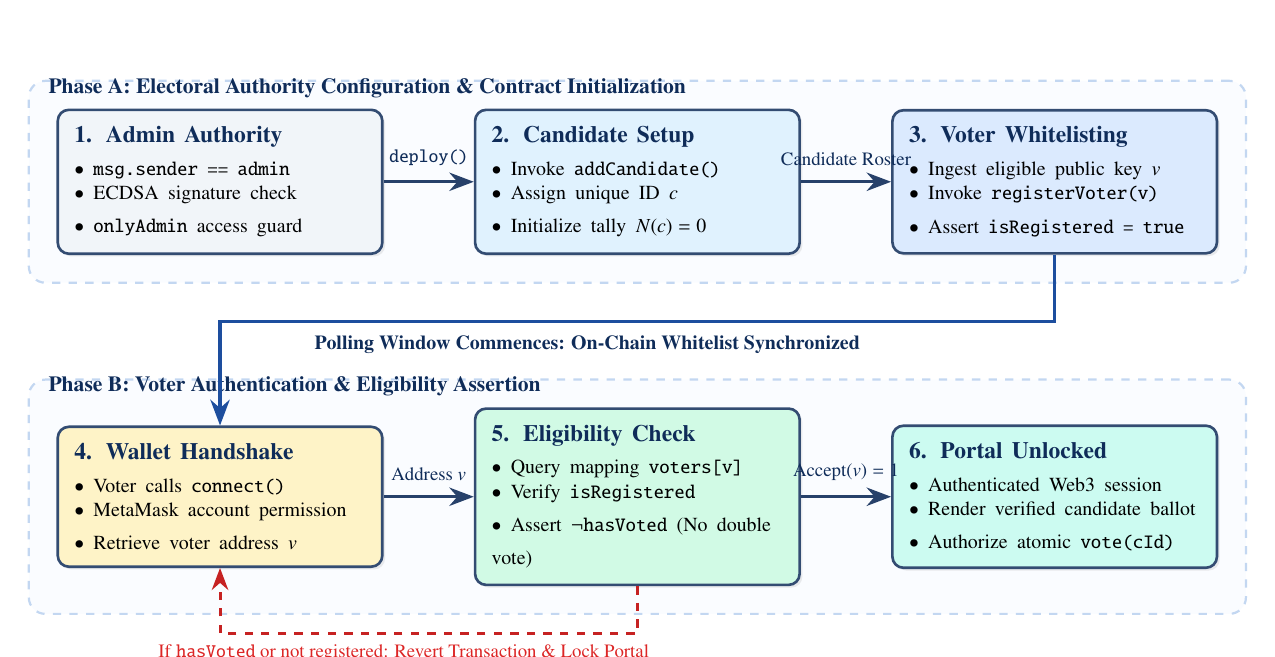
\begin{tikzpicture}[
    x=1cm, y=1cm,
    stepbox/.style={
        rectangle, draw=lavenderDark!85, line width=0.95pt, fill=white,
        rounded corners=4pt, inner sep=6pt, align=left,
        drop shadow={shadow xshift=1pt, shadow yshift=-1pt, opacity=0.15}
    },
    phasebox/.style={
        rectangle, draw=lavenderBorder!80, line width=0.8pt, fill=lavenderLight!35,
        rounded corners=6pt, inner sep=10pt, dashed
    },
    flowarr/.style={
        -{Stealth[scale=1.05]}, line width=1.2pt, draw=lavenderDark!90
    },
    dashloop/.style={
        -{Stealth[scale=1.0]}, line width=1.1pt, dashed, draw=prismBlue!90!black
    },
    revertarr/.style={
        -{Stealth[scale=1.0]}, line width=1.1pt, dashed, draw=statusFail!90!black
    }
]

    % =========================================================================
    % ROW 1: ADMINISTRATOR ELECTION SETUP PHASE
    % =========================================================================
    
    % Step 1: Admin Authority Verification
    \node [stepbox, fill=cInput, text width=3.7cm] (b1) at (-5.3, 2.0) {
        {\fontsize{8.5}{10.5}\selectfont\bfseries\color{lavenderDark}1. Admin Authority}\\[0.3em]
        \fontsize{7.2}{8.8}\selectfont
        $\bullet$ \texttt{msg.sender == admin}\\
        $\bullet$ ECDSA signature check\\
        $\bullet$ \texttt{onlyAdmin} access guard
    };

    % Step 2: Candidate Management
    \node [stepbox, fill=cStem, text width=3.7cm] (b2) at (0.0, 2.0) {
        {\fontsize{8.5}{10.5}\selectfont\bfseries\color{lavenderDark}2. Candidate Setup}\\[0.3em]
        \fontsize{7.2}{8.8}\selectfont
        $\bullet$ Invoke \texttt{addCandidate()}\\
        $\bullet$ Assign unique ID $c$\\
        $\bullet$ Initialize tally $N(c)=0$
    };

    % Step 3: Voter Whitelisting
    \node [stepbox, fill=cHead, text width=3.7cm] (b3) at (5.3, 2.0) {
        {\fontsize{8.5}{10.5}\selectfont\bfseries\color{lavenderDark}3. Voter Whitelisting}\\[0.3em]
        \fontsize{7.2}{8.8}\selectfont
        $\bullet$ Ingest eligible public key $v$\\
        $\bullet$ Invoke \texttt{registerVoter(v)}\\
        $\bullet$ Assert \texttt{isRegistered = true}
    };

    % Phase 1 Background Box
    \begin{scope}[on background layer]
        \node [phasebox, fit=(b1)(b2)(b3), label={[font=\fontsize{7.8}{9.5}\selectfont\bfseries\color{lavenderDark}, anchor=west, xshift=4pt, yshift=-3pt]north west:Phase A: Electoral Authority Configuration \& Contract Initialization}] (p1) {};
    \end{scope}

    % Row 1 Connectors
    \draw [flowarr] (b1) -- node[above=2pt, font=\fontsize{6.8}{8.0}\selectfont, text=prismNavy] {\texttt{deploy()}} (b2);
    \draw [flowarr] (b2) -- node[above=2pt, font=\fontsize{6.8}{8.0}\selectfont, text=prismNavy] {Candidate Roster} (b3);

    % =========================================================================
    % ROW 2: VOTER AUTHENTICATION & ELIGIBILITY VERIFICATION PHASE
    % =========================================================================

    % Step 4: MetaMask Handshake
    \node [stepbox, fill=cStage2, text width=3.7cm] (b4) at (-5.3, -2.0) {
        {\fontsize{8.5}{10.5}\selectfont\bfseries\color{lavenderDark}4. Wallet Handshake}\\[0.3em]
        \fontsize{7.2}{8.8}\selectfont
        $\bullet$ Voter calls \texttt{connect()}\\
        $\bullet$ MetaMask account permission\\
        $\bullet$ Retrieve voter address $v$
    };

    % Step 5: Eligibility Verification
    \node [stepbox, fill=cStage1, text width=3.7cm] (b5) at (0.0, -2.0) {
        {\fontsize{8.5}{10.5}\selectfont\bfseries\color{lavenderDark}5. Eligibility Check}\\[0.3em]
        \fontsize{7.2}{8.8}\selectfont
        $\bullet$ Query mapping \texttt{voters[v]}\\
        $\bullet$ Verify \texttt{isRegistered}\\
        $\bullet$ Assert $\neg\texttt{hasVoted}$ (No double vote)
    };

    % Step 6: Portal Access Unlocked
    \node [stepbox, fill=cDeliverable, text width=3.7cm] (b6) at (5.3, -2.0) {
        {\fontsize{8.5}{10.5}\selectfont\bfseries\color{lavenderDark}6. Portal Unlocked}\\[0.3em]
        \fontsize{7.2}{8.8}\selectfont
        $\bullet$ Authenticated Web3 session\\
        $\bullet$ Render verified candidate ballot\\
        $\bullet$ Authorize atomic \texttt{vote(cId)}
    };

    % Phase 2 Background Box
    \begin{scope}[on background layer]
        \node [phasebox, fit=(b4)(b5)(b6), label={[font=\fontsize{7.8}{9.5}\selectfont\bfseries\color{lavenderDark}, anchor=west, xshift=4pt, yshift=-3pt]north west:Phase B: Voter Authentication \& Eligibility Assertion}] (p2) {};
    \end{scope}

    % Row 2 Connectors
    \draw [flowarr] (b4) -- node[above=2pt, font=\fontsize{6.8}{8.0}\selectfont, text=prismNavy] {Address $v$} (b5);
    \draw [flowarr] (b5) -- node[above=2pt, font=\fontsize{6.8}{8.0}\selectfont, text=prismNavy] {$\text{Accept}(v)=1$} (b6);

    % =========================================================================
    % INTER-PHASE CONNECTORS & FEEDBACK
    % =========================================================================

    % Transition from Phase A to Phase B
    \draw [flowarr, line width=1.3pt, draw=prismBlue] (b3.south) -- ++(0,-0.85) -| (b4.north)
        node[pos=0.28, below=1pt, font=\fontsize{7.2}{8.8}\selectfont\bfseries, text=prismNavy] {Polling Window Commences: On-Chain Whitelist Synchronized};

    % Revert / Double-Voting Defense Branch
    \draw [revertarr] (b5.south) -- ++(0,-0.6) -| node[pos=0.28, below, font=\fontsize{6.8}{8.0}\selectfont, text=statusFail] {If \texttt{hasVoted} or not registered: Revert Transaction \& Lock Portal} (b4.south);

\end{tikzpicture}
\end{document}
}
\caption{Detailed layered workflow for voter whitelisting, MetaMask connection, and eligibility verification.}
\label{fig:voter_workflow}
\end{figure}

\section{End-to-End Ballot Sequence Flow}
Figure~\ref{fig:end_to_end_flow} illustrates the end-to-end transaction lifecycle across the four interacting system entities: the Voter \& MetaMask Client, the React \& Web3.js Middleware, the Smart Contract on the EVM, and the Consensus Ledger.

\begin{figure}[H]
\centering
\adjustbox{max width=0.98\linewidth, max height=0.72\textheight, keepaspectratio, center}{\documentclass[tikz,border=8pt]{standalone}
\usepackage{tikz}
\usepackage{fontawesome5}
\usepackage{amsmath,amssymb}
\usetikzlibrary{arrows.meta,positioning,fit,backgrounds,calc,shadows,shapes.geometric}

% Color definitions
\definecolor{lavenderDark}{RGB}{15, 44, 89}
\definecolor{lavenderDeep}{RGB}{10, 28, 58}
\definecolor{lavenderMedium}{RGB}{29, 78, 158}
\definecolor{lavenderLight}{RGB}{240, 246, 255}
\definecolor{lavenderBorder}{RGB}{180, 205, 237}
\definecolor{lavenderAccent}{RGB}{2, 132, 199}
\definecolor{prismNavy}{RGB}{15, 44, 89}
\definecolor{prismBlue}{RGB}{29, 78, 158}
\definecolor{prismTeal}{RGB}{13, 148, 136}
\definecolor{prismMint}{RGB}{236, 253, 245}
\definecolor{prismGold}{RGB}{217, 119, 6}
\definecolor{prismDark}{RGB}{15, 23, 42}
\definecolor{prismLight}{RGB}{248, 250, 252}
\definecolor{cInput}{RGB}{241, 245, 249}
\definecolor{cStem}{RGB}{224, 242, 254}
\definecolor{cStage1}{RGB}{209, 250, 229}
\definecolor{cStage2}{RGB}{254, 243, 199}
\definecolor{cStage3}{RGB}{254, 226, 226}
\definecolor{cStage4}{RGB}{207, 250, 254}
\definecolor{cHead}{RGB}{219, 234, 254}
\definecolor{cOutput}{RGB}{255, 228, 230}
\definecolor{cDeliverable}{RGB}{204, 251, 241}
\definecolor{statusFail}{RGB}{220, 38, 38}

\begin{document}
% End-to-End System Flow for Blockchain Voting DApp
\begin{tikzpicture}[
    x=1cm, y=1cm,
    hdrbox/.style={
        rectangle, draw=lavenderDark!80, line width=0.85pt, fill=lavenderDark!14,
        rounded corners=3pt, inner sep=4pt, align=center,
        text width=3.80cm,
        font=\fontsize{8.2}{9.8}\selectfont\bfseries\color{lavenderDark}
    },
    stepbox/.style={
        rectangle, draw=black!70, line width=0.7pt, fill=white,
        rounded corners=3pt, inner sep=3.8pt, align=center,
        text width=3.80cm,
        font=\fontsize{7.2}{8.5}\selectfont
    },
    stagebox/.style={
        rectangle, draw=lavenderDark!40, dashed, rounded corners=5pt, line width=0.8pt,
        fill=lavenderLight!25, inner xsep=5pt, inner ysep=6pt
    },
    transarr/.style={
        -{Stealth[length=4.5pt, width=3.5pt]}, line width=1.1pt, draw=lavenderMedium
    }
]

    % Column 1: Voter & MetaMask Client
    \node[hdrbox, fill=cInput] (c1_hdr) at (0, 0) {\faUser\ \textbf{Voter \& MetaMask}};
    \node[stepbox, below=0.6cm of c1_hdr] (s1_1) {
        \textbf{Access Voting Portal}\\
        Open \texttt{voting.html} in browser
    };
    \node[stepbox, below=0.6cm of s1_1] (s1_2) {
        \textbf{Connect MetaMask}\\
        Approve account access \& provide public address $v$
    };
    \node[stepbox, below=0.6cm of s1_2] (s1_3) {
        \textbf{Select Candidate $c$}\\
        Choose desired ballot option \& click Vote
    };
    \node[stepbox, below=0.6cm of s1_3] (s1_4) {
        \textbf{Sign Transaction}\\
        Cryptographically sign $\text{vote}(c)$ with ECDSA private key
    };

    % Column 2: Web3.js Middleware & RPC
    \node[hdrbox, fill=cStem, right=0.9cm of c1_hdr] (c2_hdr) {\faCode\ \textbf{React \& Web3.js}};
    \node[stepbox, below=0.6cm of c2_hdr] (s2_1) {
        \textbf{Fetch Candidates}\\
        Query contract for certified candidate array
    };
    \node[stepbox, below=0.6cm of s2_1] (s2_2) {
        \textbf{Local Pre-Validation}\\
        Verify voter status via \texttt{voters[address]}
    };
    \node[stepbox, below=0.6cm of s2_2] (s2_3) {
        \textbf{Construct Payload}\\
        Encode ABI invocation \texttt{vote(candidateId)}
    };
    \node[stepbox, below=0.6cm of s2_3] (s2_4) {
        \textbf{Relay via JSON-RPC}\\
        Broadcast raw signed transaction to Ethereum node
    };

    % Column 3: Smart Contract (EVM)
    \node[hdrbox, fill=cStage2, right=0.9cm of c2_hdr] (c3_hdr) {\faFileContract\ \textbf{Smart Contract (EVM)}};
    \node[stepbox, below=0.6cm of c3_hdr] (s3_1) {
        \textbf{Registration Check}\\
        \texttt{require(registered[v])}\\
        \textit{Revert if unauthorized}
    };
    \node[stepbox, below=0.6cm of s3_1] (s3_2) {
        \textbf{Double-Voting Mitigation}\\
        \texttt{require(!voters[v].hasVoted)}\\
        \textit{Atomic check $\text{Accept}(v)$}
    };
    \node[stepbox, below=0.6cm of s3_2] (s3_3) {
        \textbf{State Mutation}\\
        \texttt{voters[v].hasVoted = true}\\
        \texttt{candidates[c].voteCount++}
    };
    \node[stepbox, below=0.6cm of s3_3] (s3_4) {
        \textbf{Emit Event}\\
        \texttt{emit VoteCast(v, c, block.timestamp)}
    };

    % Column 4: Blockchain Ledger & Consensus
    \node[hdrbox, fill=cDeliverable, right=0.9cm of c3_hdr] (c4_hdr) {\faCube\ \textbf{Consensus \& Ledger}};
    \node[stepbox, below=0.6cm of c4_hdr] (s4_1) {
        \textbf{Mempool Ingestion}\\
        Transaction queued in pending validator pool
    };
    \node[stepbox, below=0.6cm of s4_1] (s4_2) {
        \textbf{PoA Block Sealing}\\
        Block mined by designated validator node
    };
    \node[stepbox, below=0.6cm of s4_2] (s4_3) {
        \textbf{Cryptographic Hash Chaining}\\
        $H(B_i) = \text{SHA-256}(H(B_{i-1}) \parallel \dots)$
    };
    \node[stepbox, below=0.6cm of s4_3] (s4_4) {
        \textbf{Immutable Receipt}\\
        Tx confirmed; Event captured by Web3 dashboard
    };

    % Background Stage Boxes
    \begin{scope}[on background layer]
        \node[stagebox, fit=(c1_hdr)(s1_4)] (col1_box) {};
        \node[stagebox, fit=(c2_hdr)(s2_4)] (col2_box) {};
        \node[stagebox, fit=(c3_hdr)(s3_4)] (col3_box) {};
        \node[stagebox, fit=(c4_hdr)(s4_4)] (col4_box) {};
    \end{scope}

    % Transition arrows across columns
    \draw[transarr] (s1_1) -- (s2_1);
    \draw[transarr] (s1_2) -- (s2_2);
    \draw[transarr] (s1_3) -- (s2_3);
    \draw[transarr] (s1_4) -- (s2_4);
    \draw[transarr] (s2_4) -- (s3_1);
    \draw[transarr] (s3_1) -- (s3_2);
    \draw[transarr] (s3_2) -- (s3_3);
    \draw[transarr] (s3_3) -- (s3_4);
    \draw[transarr] (s3_4) -- (s4_1);
    \draw[transarr] (s4_1) -- (s4_2);
    \draw[transarr] (s4_2) -- (s4_3);
    \draw[transarr] (s4_3) -- (s4_4);

    % Event Feedback Arrow to React
    \draw[transarr, dashed, draw=prismTeal] (s4_4.south) -- ++(0,-0.4) -| (s2_4.south)
        node[pos=0.25, below, font=\fontsize{6.5}{7.5}\selectfont, text=prismNavy] {Web3 Event Notification \& Real-Time UI Tally Update};

\end{tikzpicture}
\end{document}
}
\caption{End-to-end system sequence flow from ballot selection to block sealing and real-time Web3 tally notification.}
\label{fig:end_to_end_flow}
\end{figure}

\section{Complete System Operational Flowchart}
Figure~\ref{fig:sys_flowchart} depicts the complete operational flowchart of the voting decentralized application, detailing role verification, whitelisting validation, double-voting rejection branches, and event emissions.

\begin{figure}[H]
\centering
\adjustbox{max width=0.98\linewidth, max height=0.72\textheight, keepaspectratio, center}{\documentclass[tikz,border=10pt]{standalone}
\usepackage{tikz}
\usepackage{fontawesome5}
\usepackage{amsmath,amssymb}
\usetikzlibrary{arrows.meta,positioning,fit,backgrounds,calc,shadows,shapes.geometric}

% Color definitions
\definecolor{lavenderDark}{RGB}{15, 44, 89}
\definecolor{lavenderDeep}{RGB}{10, 28, 58}
\definecolor{lavenderMedium}{RGB}{29, 78, 158}
\definecolor{lavenderLight}{RGB}{240, 246, 255}
\definecolor{lavenderBorder}{RGB}{180, 205, 237}
\definecolor{prismNavy}{RGB}{15, 44, 89}
\definecolor{prismBlue}{RGB}{29, 78, 158}
\definecolor{prismTeal}{RGB}{13, 148, 136}
\definecolor{prismGold}{RGB}{217, 119, 6}
\definecolor{prismDark}{RGB}{15, 23, 42}
\definecolor{statusFail}{RGB}{220, 38, 38}
\definecolor{cInput}{RGB}{241, 245, 249}
\definecolor{cStem}{RGB}{224, 242, 254}
\definecolor{cStage1}{RGB}{209, 250, 229}
\definecolor{cStage2}{RGB}{254, 243, 199}
\definecolor{cHead}{RGB}{219, 234, 254}

\begin{document}
% Complete Flowchart for Blockchain Voting DApp & Double-Voting Mitigation
\begin{tikzpicture}[
  x=1cm, y=1cm,
  startend/.style={
    ellipse, draw=green!60!black, fill=green!45!black, text=white,
    line width=0.9pt, inner sep=3.5pt, font=\fontsize{7.5}{8.5}\selectfont\bfseries,
    minimum width=1.80cm, minimum height=0.60cm, drop shadow={opacity=0.12}
  },
  procbox/.style={
    rectangle, rounded corners=3.5pt,
    draw=lavenderDark!80, fill=white, text=black,
    line width=0.85pt, inner sep=4.0pt, font=\fontsize{7.0}{8.2}\selectfont,
    minimum height=0.75cm, text width=3.30cm, align=center, drop shadow={opacity=0.10}
  },
  decision/.style={
    diamond, aspect=2.0,
    draw=prismNavy, fill=lavenderLight, text=prismNavy,
    line width=0.85pt, inner sep=2.5pt, font=\fontsize{6.5}{7.6}\selectfont\bfseries,
    align=center, drop shadow={opacity=0.10}
  },
  errorbox/.style={
    rectangle, rounded corners=3pt,
    draw=statusFail!80, fill=statusFail!12, text=statusFail!90!black,
    line width=0.80pt, inner sep=3.5pt, font=\fontsize{6.5}{7.5}\selectfont\bfseries,
    minimum height=0.65cm, text width=2.40cm, align=center
  },
  flowarr/.style={
    -{Stealth[scale=0.85]}, line width=0.85pt, draw=lavenderDark!90
  },
  failarr/.style={
    -{Stealth[scale=0.80]}, line width=0.80pt, draw=statusFail!90, dashed
  }
]

  % Start
  \node[startend] (start) at (0, 0) {START};

  % Connect Wallet
  \node[procbox, fill=cInput, below=0.55cm of start] (connect) {
    \textbf{MetaMask Handshake}\\
    Request account access (\texttt{msg.sender})
  };

  % Decision 1: Is Admin?
  \node[decision, below=0.60cm of connect] (d_admin) {
    Is Caller\\Administrator?
  };

  % Admin Branch (Left)
  \node[procbox, fill=cStem, left=1.2cm of d_admin] (admin_portal) {
    \textbf{Admin Dashboard}\\
    Access \texttt{admin.html}
  };
  \node[procbox, fill=cHead, below=0.70cm of admin_portal] (admin_ops) {
    \textbf{Administrative Actions}\\
    $\bullet$ \texttt{addCandidate(name)}\\
    $\bullet$ \texttt{registerVoter(address)}
  };
  \node[procbox, fill=cStage1, below=0.70cm of admin_ops] (admin_commit) {
    \textbf{EVM State Update}\\
    Update candidate array /\\
    whitelist mapping
  };

  % Voter Branch: Check Registered
  \node[decision, below=0.75cm of d_admin] (d_reg) {
    Is Address\\Whitelisted?
  };
  \node[errorbox, right=1.2cm of d_reg] (err_reg) {
    \faTimesCircle\ REVERT:\\
    Unregistered Voter
  };

  % Voter Branch: Check Already Voted
  \node[decision, below=0.75cm of d_reg] (d_voted) {
    Has Address\\Already Voted?
  };
  \node[errorbox, right=1.2cm of d_voted] (err_voted) {
    \faBan\ REVERT:\\
    Double Vote Rejected
  };

  % Ballot Casting
  \node[procbox, fill=cStem, below=0.75cm of d_voted] (ballot_view) {
    \textbf{Display Ballot Portal}\\
    Show certified candidate list
  };
  \node[procbox, fill=cStage2, below=0.55cm of ballot_view] (sign_tx) {
    \textbf{Sign Ballot Transaction}\\
    Voter confirms candidate $c$ in MetaMask
  };
  \node[procbox, fill=cStage1, below=0.55cm of sign_tx] (atomic_evm) {
    \textbf{Atomic EVM Execution}\\
    \texttt{voters[v].hasVoted = true}\\
    \texttt{candidates[c].voteCount++}
  };
  \node[procbox, fill=cHead, below=0.55cm of atomic_evm] (emit_event) {
    \textbf{Block Seal \& Event Broadcast}\\
    PoA consensus commits block $B_i$\\
    Emit \texttt{VoteCast} event
  };

  % End
  \node[startend, below=0.55cm of emit_event] (finish) {END};

  % Routing arrows
  \draw[flowarr] (start) -- (connect);
  \draw[flowarr] (connect) -- (d_admin);

  \draw[flowarr] (d_admin) -- node[above, font=\tiny\bfseries] {YES} (admin_portal);
  \draw[flowarr] (admin_portal) -- (admin_ops);
  \draw[flowarr] (admin_ops) -- (admin_commit);
  \draw[flowarr] (admin_commit) |- (finish);

  \draw[flowarr] (d_admin) -- node[right, font=\tiny\bfseries] {NO} (d_reg);
  \draw[failarr] (d_reg) -- node[above, font=\tiny\bfseries] {NO} (err_reg);
  \draw[flowarr] (d_reg) -- node[right, font=\tiny\bfseries] {YES} (d_voted);

  \draw[failarr] (d_voted) -- node[above, font=\tiny\bfseries] {YES} (err_voted);
  \draw[flowarr] (d_voted) -- node[right, font=\tiny\bfseries] {NO} (ballot_view);

  \draw[flowarr] (ballot_view) -- (sign_tx);
  \draw[flowarr] (sign_tx) -- (atomic_evm);
  \draw[flowarr] (atomic_evm) -- (emit_event);
  \draw[flowarr] (emit_event) -- (finish);

  \draw[failarr] (err_reg.east) -- ++(0.4, 0) |- (finish.east);
  \draw[failarr] (err_voted.east) -- ++(0.4, 0) |- (finish.east);

\end{tikzpicture}
\end{document}
}
\caption{Comprehensive system flowchart detailing administrator actions, voter verification branches, and atomic double-voting mitigation.}
\label{fig:sys_flowchart}
\end{figure}

\clearpage
\section{Algorithm}
The system workflow is summarized below in pseudocode.

\begin{verbatim}
ALGORITHM DecentralizedVoting
INPUT: candidate list C, voter wallet v, selected candidate c

1. Deploy contract; set admin = deployer; initialize all counts to zero.
2. ADMIN registers each candidate in C and whitelists eligible wallets.
3. VOTER connects MetaMask and obtains wallet address v.
4. record <- readVoter(v)
5. IF record.isRegistered = false OR record.hasVoted = true THEN
       deny access and stop
   END IF
6. Display candidates and let voter select c.
7. Sign vote(c) with MetaMask and submit the transaction.
8. CONTRACT checks registration, hasVoted = false, and c is valid.
9. IF any check fails THEN revert transaction and stop.
10. Set voters[v].hasVoted <- true.
11. Increment candidates[c].voteCount and emit VoteCast.
12. Commit the transaction to the blockchain and display the receipt.
13. Read final candidate tallies for public auditing.
OUTPUT: immutable vote record and auditable election tally
\end{verbatim}


\section{Block Structure and Cryptographic Chaining}
Figure~\ref{fig:block_structure} details the internal architecture of blocks within the blockchain ledger, demonstrating how block headers, cryptographic timestamps $T_i$, nonces $n_i$, and transaction sets $Tx_i$ are chained via SHA-256 hashing.

\begin{figure}[H]
\centering
\adjustbox{max width=0.98\linewidth, max height=0.55\textheight, keepaspectratio, center}{\documentclass[tikz,border=10pt]{standalone}
\usepackage{tikz}
\usepackage{fontawesome5}
\usepackage{amsmath,amssymb}
\usetikzlibrary{arrows.meta,positioning,fit,backgrounds,calc,shadows,shapes.geometric}

% Color definitions
\definecolor{lavenderDark}{RGB}{15, 44, 89}
\definecolor{lavenderDeep}{RGB}{10, 28, 58}
\definecolor{lavenderMedium}{RGB}{29, 78, 158}
\definecolor{lavenderLight}{RGB}{240, 246, 255}
\definecolor{lavenderBorder}{RGB}{180, 205, 237}
\definecolor{prismNavy}{RGB}{15, 44, 89}
\definecolor{prismBlue}{RGB}{29, 78, 158}
\definecolor{prismTeal}{RGB}{13, 148, 136}
\definecolor{prismGold}{RGB}{217, 119, 6}
\definecolor{prismDark}{RGB}{15, 23, 42}
\definecolor{prismSlate}{RGB}{100, 116, 139}
\definecolor{statusFail}{RGB}{220, 38, 38}
\definecolor{cInput}{RGB}{241, 245, 249}
\definecolor{cStem}{RGB}{224, 242, 254}
\definecolor{cStage1}{RGB}{209, 250, 229}
\definecolor{cStage2}{RGB}{254, 243, 199}
\definecolor{cHead}{RGB}{219, 234, 254}

\begin{document}
% Blockchain Block Structure and Cryptographic Chaining Diagram
\begin{tikzpicture}[
  x=1cm, y=1cm,
  blockcard/.style={
    rectangle, rounded corners=6pt, draw=lavenderDark!90, line width=1.1pt,
    fill=white, text width=4.60cm, minimum height=6.20cm,
    inner sep=6pt, drop shadow={shadow xshift=1.2pt, shadow yshift=-1.2pt, opacity=0.15}
  },
  hdrsub/.style={
    rectangle, rounded corners=3pt, draw=prismBlue!70, fill=cStem,
    text width=4.30cm, inner sep=4pt, align=left, font=\fontsize{6.8}{8.0}\selectfont
  },
  txsub/.style={
    rectangle, rounded corners=3pt, draw=prismTeal!70, fill=cStage1,
    text width=4.30cm, inner sep=4pt, align=left, font=\fontsize{6.6}{7.8}\selectfont
  },
  hashsub/.style={
    rectangle, rounded corners=3pt, draw=prismGold!80, fill=cStage2,
    text width=4.30cm, inner sep=4pt, align=left, font=\fontsize{6.8}{8.0}\selectfont
  },
  chainarr/.style={
    -{Stealth[scale=1.1]}, line width=1.6pt, draw=lavenderDark
  }
]

  %============================================================================
  % BLOCK i-1
  %============================================================================
  \node[blockcard] (b_prev) at (-5.4, 0) {};
  \node[anchor=north, font=\fontsize{8.5}{10.5}\selectfont\bfseries, text=prismNavy] at ([yshift=-4pt]b_prev.north) {
    \faCube\ \textbf{BLOCK} $B_{i-1}$ \textit{(Previous)}
  };
  \node[hdrsub, below=0.6cm of b_prev.north] (h_prev) {
    \textbf{Block Header:}\\[1.5pt]
    $\bullet$ Prev Hash: \texttt{0x9f7a...3c21}\\
    $\bullet$ Timestamp: $T_{i-1} = 1730001200$\\
    $\bullet$ Nonce: $n_{i-1} = 48219$\\
    $\bullet$ Merkle Root: \texttt{0x4e8b...1a02}
  };
  \node[txsub, below=0.35cm of h_prev] (tx_prev) {
    \textbf{Transactions} ($Tx_{i-1}$):\\[1.5pt]
    \texttt{Tx1}: Voter $h(v_a) \to$ Cand.\ $c_1$ [Signed]\\
    \texttt{Tx2}: Voter $h(v_b) \to$ Cand.\ $c_2$ [Signed]\\
    \texttt{Tx3}: Voter $h(v_c) \to$ Cand.\ $c_1$ [Signed]
  };
  \node[hashsub, below=0.35cm of tx_prev] (hash_prev) {
    \textbf{Block Hash} $H(B_{i-1})$:\\[1.5pt]
    \texttt{0x2b8c9d1e...f7a34510}\\
    \textit{SHA-256 Digest of Block Body \& Header}
  };

  %============================================================================
  % BLOCK i
  %============================================================================
  \node[blockcard] (b_curr) at (0, 0) {};
  \node[anchor=north, font=\fontsize{8.5}{10.5}\selectfont\bfseries, text=prismNavy] at ([yshift=-4pt]b_curr.north) {
    \faCube\ \textbf{BLOCK} $B_i$ \textit{(Current Validated)}
  };
  \node[hdrsub, below=0.6cm of b_curr.north] (h_curr) {
    \textbf{Block Header:}\\[1.5pt]
    $\bullet$ Prev Hash: \textbf{\texttt{0x2b8c...4510}}\\
    $\bullet$ Timestamp: $T_i = 1730001215$\\
    $\bullet$ Nonce: $n_i = 91823$\\
    $\bullet$ Merkle Root: \texttt{0x7a3f...9d81}
  };
  \node[txsub, below=0.35cm of h_curr] (tx_curr) {
    \textbf{Transactions} ($Tx_i$):\\[1.5pt]
    \texttt{Tx1}: Voter $h(v_d) \to$ Cand.\ $c_3$ [Signed]\\
    \texttt{Tx2}: Voter $h(v_e) \to$ Cand.\ $c_1$ [Signed]\\
    \texttt{Tx3}: Voter $h(v_f) \to$ Cand.\ $c_2$ [Signed]
  };
  \node[hashsub, below=0.35cm of tx_curr] (hash_curr) {
    \textbf{Block Hash} $H(B_i)$:\\[1.5pt]
    $H(B_i) = \text{SHA-256}(H(B_{i-1}) \parallel T_i \parallel Tx_i \parallel n_i)$\\[1.5pt]
    \textbf{\texttt{0x6e4a19b8...c3d821f9}}
  };

  %============================================================================
  % BLOCK i+1
  %============================================================================
  \node[blockcard] (b_next) at (5.4, 0) {};
  \node[anchor=north, font=\fontsize{8.5}{10.5}\selectfont\bfseries, text=prismNavy] at ([yshift=-4pt]b_next.north) {
    \faCube\ \textbf{BLOCK} $B_{i+1}$ \textit{(Subsequent)}
  };
  \node[hdrsub, below=0.6cm of b_next.north] (h_next) {
    \textbf{Block Header:}\\[1.5pt]
    $\bullet$ Prev Hash: \textbf{\texttt{0x6e4a...21f9}}\\
    $\bullet$ Timestamp: $T_{i+1} = 1730001230$\\
    $\bullet$ Nonce: $n_{i+1} = 14205$\\
    $\bullet$ Merkle Root: \texttt{0x3c21...8e90}
  };
  \node[txsub, below=0.35cm of h_next] (tx_next) {
    \textbf{Transactions} ($Tx_{i+1}$):\\[1.5pt]
    \texttt{Tx1}: Voter $h(v_g) \to$ Cand.\ $c_2$ [Signed]\\
    \texttt{Tx2}: Voter $h(v_h) \to$ Cand.\ $c_1$ [Signed]\\
    \texttt{Tx3}: Voter $h(v_i) \to$ Cand.\ $c_3$ [Signed]
  };
  \node[hashsub, below=0.35cm of tx_next] (hash_next) {
    \textbf{Block Hash} $H(B_{i+1})$:\\[1.5pt]
    \texttt{0x8d5c7b3e...9a4102ef}\\
    \textit{Guaranteed Immutable Ledger State}
  };

  % Cryptographic hash linkage arrows
  \draw[chainarr] (hash_prev.east) to[out=0, in=180] (h_curr.west);
  \draw[chainarr] (hash_curr.east) to[out=0, in=180] (h_next.west);

\end{tikzpicture}
\end{document}
}
\caption{Cryptographic block structure and hash chaining mechanism illustrating ledger immutability.}
\label{fig:block_structure}
\end{figure}

The cryptographic linking between consecutive blocks $B_{i-1}$ and $B_i$ guarantees that historical records cannot be retroactively modified without invalidating all downstream block hashes. Each block encapsulates the Merkle root summarizing its transaction set $Tx_i$, ensuring that any attempted alteration of a single cast vote invalidates the entire block header digest.

\section{Smart Contract State Schemas and Structs}
Figure~\ref{fig:db_schema} depicts the relational entity connections, state mapping layouts, and event logging structures organized across three primary architectural tiers in the Solidity smart contract.

\begin{figure}[H]
\centering
\vspace{-0.5em}
\adjustbox{max width=0.98\linewidth, max height=0.36\textheight, keepaspectratio, center}{\documentclass[tikz,border=10pt]{standalone}
\usepackage{tikz}
\usepackage{fontawesome5}
\usepackage{amsmath,amssymb}
\usetikzlibrary{arrows.meta,positioning,fit,backgrounds,calc,shadows,shapes.geometric}

% Color definitions
\definecolor{lavenderDark}{RGB}{15, 44, 89}
\definecolor{lavenderDeep}{RGB}{10, 28, 58}
\definecolor{lavenderMedium}{RGB}{29, 78, 158}
\definecolor{lavenderLight}{RGB}{240, 246, 255}
\definecolor{lavenderBorder}{RGB}{180, 205, 237}
\definecolor{prismNavy}{RGB}{15, 44, 89}
\definecolor{prismBlue}{RGB}{29, 78, 158}
\definecolor{prismTeal}{RGB}{13, 148, 136}
\definecolor{prismMint}{RGB}{236, 253, 245}
\definecolor{prismGold}{RGB}{217, 119, 6}
\definecolor{prismDark}{RGB}{15, 23, 42}
\definecolor{prismSlate}{RGB}{100, 116, 139}
\definecolor{statusFail}{RGB}{220, 38, 38}
\definecolor{cStem}{RGB}{224, 242, 254}
\definecolor{cStage1}{RGB}{209, 250, 229}
\definecolor{cHead}{RGB}{219, 234, 254}
\definecolor{cDeliverable}{RGB}{204, 251, 241}

\begin{document}
\begin{tikzpicture}[
  x=1cm, y=1cm,
  tblcard/.style={
    rectangle, rounded corners=4pt, draw=lavenderDark!80, line width=0.85pt, fill=white,
    inner sep=5pt, text width=4.70cm, align=left,
    drop shadow={shadow xshift=1pt, shadow yshift=-1pt, opacity=0.10}
  },
  fkarrow/.style={
    -{Stealth[scale=0.95]}, line width=1.1pt, draw=lavenderDark!90
  },
  fklabel/.style={
    font=\fontsize{6.8}{8.0}\selectfont\bfseries, fill=white, inner sep=1.8pt, text=lavenderDark, draw=lavenderBorder, line width=0.5pt, rounded corners=2pt
  }
]

  % ================= COLUMN 1: VOTER & ADMIN (x = -4.5) =================
  
  % Table 1: Voter Struct
  \node[tblcard, fill=cStem!45] (voter) at (-4.5, 1.9) {%
    \centerline{\color{lavenderDark}\faUserCheck\ \textbf{\fontsize{8.5}{10.0}\selectfont struct Voter}}\\[2pt]
    \rule{\linewidth}{0.4pt}\\[2pt]
    {\fontsize{7.2}{8.8}\selectfont
    \textbf{\color{lavenderDark}[KEY]} \texttt{address}: \textit{address} (160-bit hex)\\
    \textbf{\color{prismTeal}[STATE]} \texttt{isRegistered}: \textit{bool}\\
    \textbf{\color{statusFail!90!black}[STATE]} \texttt{hasVoted}: \textit{bool} (Atomic flag)\\
    \textbf{\color{prismBlue}[FK]} \texttt{votedCandidateId}: \textit{uint}\\
    \textbf{\color{prismDark!80}[FLD]} \texttt{voteTimestamp}: \textit{uint256}}
  };

  % Table 2: Election Admin & Config
  \node[tblcard, below=0.65cm of voter, fill=cHead!45] (admin) {%
    \centerline{\color{lavenderDark}\faUserShield\ \textbf{\fontsize{8.5}{10.0}\selectfont contract ElectionState}}\\[2pt]
    \rule{\linewidth}{0.4pt}\\[2pt]
    {\fontsize{7.2}{8.8}\selectfont
    \textbf{\color{lavenderDark}[OWNER]} \texttt{admin}: \textit{address} (Contract owner)\\
    \textbf{\color{prismDark!80}[MAP]} \texttt{voters}: \textit{mapping(address $\Rightarrow$ Voter)}\\
    \textbf{\color{prismDark!80}[ARR]} \texttt{candidates}: \textit{Candidate[]}\\
    \textbf{\color{prismTeal}[CNT]} \texttt{candidatesCount}: \textit{uint}\\
    \textbf{\color{prismGold}[CNT]} \texttt{totalVotesTallied}: \textit{uint256}}
  };

  % ================= COLUMN 2: CANDIDATE & LEDGER RECEIPT (x = 4.5) =================

  % Table 3: Candidate Struct
  \node[tblcard, fill=cStage1!45] (candidate) at (4.5, 1.9) {%
    \centerline{\color{lavenderDark}\faVoteYea\ \textbf{\fontsize{8.5}{10.0}\selectfont struct Candidate}}\\[2pt]
    \rule{\linewidth}{0.4pt}\\[2pt]
    {\fontsize{7.2}{8.8}\selectfont
    \textbf{\color{lavenderDark}[PK]} \texttt{id}: \textit{uint} (Unique candidate ID)\\
    \textbf{\color{prismDark!80}[FLD]} \texttt{name}: \textit{string} (Candidate Moniker)\\
    \textbf{\color{prismTeal}[TALLY]} \texttt{voteCount}: \textit{uint} (Total $N(c)$)\\
    \textbf{\color{prismBlue}[AUDIT]} \texttt{registrationBlock}: \textit{uint256}\\
    \textbf{\color{prismGold}[VAL]} \texttt{isValid}: \textit{bool}}
  };

  % Table 4: Transaction & Event Receipt
  \node[tblcard, below=0.65cm of candidate, fill=cDeliverable!55] (receipt) {%
    \centerline{\color{lavenderDark}\faReceipt\ \textbf{\fontsize{8.5}{10.0}\selectfont event VoteCast \& Receipt}}\\[2pt]
    \rule{\linewidth}{0.4pt}\\[2pt]
    {\fontsize{7.2}{8.8}\selectfont
    \textbf{\color{lavenderDark}[HASH]} \texttt{txHash}: \textit{bytes32} (Keccak-256)\\
    \textbf{\color{prismBlue}[IDX]} \texttt{voter}: \textit{address} (Indexed sender)\\
    \textbf{\color{prismTeal}[IDX]} \texttt{candidateId}: \textit{uint} (Indexed choice)\\
    \textbf{\color{prismDark!80}[BLK]} \texttt{blockNumber}: \textit{uint256}\\
    \textbf{\color{prismGold}[SEAL]} \texttt{blockHash}: \textit{bytes32}}
  };

  % Foreign Key & Relational Connectors
  \draw[fkarrow] (voter.east) -- (candidate.west)
    node[midway, fklabel] {votes for candidateId};

  \draw[fkarrow] (admin.north) -- (voter.south)
    node[midway, fklabel] {manages whitelist};

  \draw[fkarrow] (admin.east) -- (candidate.south west)
    node[pos=0.40, fklabel, sloped] {registers Candidate};

  \draw[fkarrow] (admin.east) -- (receipt.west)
    node[midway, fklabel] {emits VoteCast};

  \draw[fkarrow] (candidate.south) -- (receipt.north)
    node[midway, fklabel] {increments voteCount};

\end{tikzpicture}
\end{document}
}
\vspace{-0.5em}
\caption{Smart contract state schemas, data structs, and relational mappings governing voters and candidates.}
\label{fig:db_schema}
\end{figure}
\vspace{-0.6em}

\noindent\textbf{Architectural State Decomposition:}
The smart contract decouples voter authorization, candidate registry, and audit logging into three distinct operational layers:
\begin{itemize}
    \setlength{\itemsep}{2pt}
    \setlength{\parskip}{0pt}
    \item \textbf{Entity Structs:} \texttt{struct Voter} enforces single-ballot casting via the atomic boolean flag \texttt{hasVoted} ($O(1)$ duplicate prevention), while \texttt{struct Candidate} maintains verified identity profiles and live vote tallies $N(c)$.
    \item \textbf{Relational Storage Mappings:} \texttt{mapping(address => Voter) public voters} provides constant-time lookup during ballot validation while safeguarding voter roster privacy. The \texttt{Candidate[] public candidates} array enables dynamic candidate onboarding and bounds checking.
    \item \textbf{Access Control and Event Emission:} Privileged administrative actions are restricted to \texttt{address public admin} via the \texttt{onlyAdmin} modifier. Each accepted ballot atomically increments $N(c)$ and emits a standardized \texttt{VoteCast} event into the EVM receipt trie for real-time, gasless auditability by external Web3 observers.
\end{itemize}
\section{Level-1 Data Flow Diagram (DFD)}
\vspace{-0.3em}
Figure~\ref{fig:dfd1} illustrates the Level-1 Data Flow Diagram (DFD) characterizing the operational data pipelines, external actor interfaces, smart contract execution routines, and persistent ledger data stores.

\begin{figure}[H]
\centering
\vspace{-0.9em}
\adjustbox{max width=0.95\linewidth, max height=0.35\textheight, keepaspectratio, center}{\documentclass[tikz,border=10pt]{standalone}
\usepackage{tikz}
\usepackage{amsmath,amssymb}
\usepackage{fontawesome5}
\usetikzlibrary{arrows.meta,positioning,fit,backgrounds,calc,shadows,shapes.geometric}

% Color definitions
\definecolor{lavenderDark}{RGB}{15, 44, 89}
\definecolor{lavenderDeep}{RGB}{10, 28, 58}
\definecolor{lavenderMedium}{RGB}{29, 78, 158}
\definecolor{lavenderLight}{RGB}{240, 246, 255}
\definecolor{lavenderBorder}{RGB}{180, 205, 237}
\definecolor{prismNavy}{RGB}{15, 44, 89}
\definecolor{prismBlue}{RGB}{29, 78, 158}
\definecolor{prismTeal}{RGB}{13, 148, 136}
\definecolor{prismGold}{RGB}{217, 119, 6}
\definecolor{prismDark}{RGB}{15, 23, 42}
\definecolor{cInput}{RGB}{241, 245, 249}
\definecolor{cStem}{RGB}{224, 242, 254}
\definecolor{cStage1}{RGB}{209, 250, 229}
\definecolor{cStage2}{RGB}{254, 243, 199}
\definecolor{cStage4}{RGB}{207, 250, 254}
\definecolor{cHead}{RGB}{219, 234, 254}

\begin{document}
% Level-1 Data Flow Diagram (DFD) for Blockchain Electronic Voting System
\begin{tikzpicture}[
  x=1.0cm, y=1.0cm,
  entity/.style={
    rectangle, draw=lavenderDark!90, line width=1.1pt, rounded corners=4pt,
    align=center, inner sep=5pt, font=\fontsize{8.5}{10.5}\selectfont\bfseries,
    text width=3.0cm, fill=cInput, drop shadow={opacity=0.12}
  },
  store/.style={
    rectangle, draw=lavenderDark!85, line width=1.1pt, rounded corners=2pt,
    align=center, inner sep=4.5pt, font=\fontsize{8.0}{9.5}\selectfont,
    text width=3.3cm, fill=lavenderLight, drop shadow={opacity=0.10}
  },
  proc/.style={
    circle, draw=lavenderMedium!95, line width=1.1pt,
    align=center, inner sep=2pt, minimum size=2.20cm,
    font=\fontsize{8.0}{9.5}\selectfont\bfseries, fill=cStage1, drop shadow={opacity=0.10}
  },
  procblue/.style={proc, fill=cStage4},
  procgold/.style={proc, fill=cStage2},
  prochead/.style={proc, fill=cHead},
  dfdarr/.style={
    -{Stealth[scale=1.0, length=5pt, width=4pt]}, line width=1.0pt, draw=lavenderDark!90
  },
  flowlbl/.style={
    font=\fontsize{7.2}{8.5}\selectfont\bfseries, fill=white, inner sep=2.0pt,
    rounded corners=2pt, text=lavenderDark, draw=lavenderBorder!70, line width=0.45pt,
    align=center
  }
]

  % External Entities (Left column and Right column)
  \node[entity] (admin) at (-7.2, 2.7) {\faUserShield\ Election\\[2pt]Administrator};
  \node[entity, fill=cStem!75] (voter) at (-7.2, -2.6) {\faUser\ Registered\\[2pt]Voter (MetaMask)};
  \node[entity, fill=cInput!70] (auditor) at (9.4, 0.0) {\faEye\ Public Auditor /\\[2pt]Observer};

  % Processes (Column 2: p1, p2; Column 3: p4, p3; Column 4: p5)
  \node[prochead] (p1) at (-2.9, 2.7) {1.0\\[1pt]Whitelist\\[1pt]\& Setup};
  \node[procblue] (p2) at (-2.9, -2.6) {2.0\\[1pt]Wallet Auth\\[1pt]\& Connect};
  \node[procgold] (p3) at (1.6, -2.6) {3.0\\[1pt]Cast Ballot\\[1pt]Transaction};
  \node[proc] (p4) at (1.6, 2.7) {4.0\\[1pt]Double-Vote\\[1pt]Mitigation};
  \node[prochead] (p5) at (5.2, 0.0) {5.0\\[1pt]Consensus\\[1pt]\& Tally};

  % Data Stores
  \node[store] (d1) at (-0.7, 0.0) {\textbf{D1: Voter Mapping}\\[2pt]\scriptsize \texttt{voters[address]}};
  \node[store] (d2) at (1.6, 4.9) {\textbf{D2: Candidates}\\[2pt]\scriptsize \texttt{candidates[]}};
  \node[store] (d3) at (5.2, -2.8) {\textbf{D3: Blockchain Ledger}\\[2pt]\scriptsize Immutable Blocks \& Receipts};

  % Admin Flows
  \draw[dfdarr] (admin) -- node[above=2pt, flowlbl] {Voter\\Addresses} (p1);
  \draw[dfdarr] (admin.north) |- node[pos=0.72, above=2pt, flowlbl] {Candidate Monikers} (d2.west);
  \draw[dfdarr] (p1.south) to[out=285, in=125] node[pos=0.48, left=3pt, flowlbl] {Register\\Flag} (d1.north west);

  % Voter Flows
  \draw[dfdarr] (voter) -- node[above=2pt, flowlbl] {Connect\\Request} (p2);
  \draw[dfdarr] (p2.north) to[out=75, in=235] node[pos=0.48, left=3pt, flowlbl] {Query\\Status} (d1.south west);
  \draw[dfdarr] (p2) -- node[above=2pt, flowlbl] {Address OK} (p3);
  \draw[dfdarr] (p3) -- node[pos=0.50, right=3pt, flowlbl] {Signed Tx} (p4);

  % Double-Vote Mitigation & Candidate Flows
  \draw[dfdarr] (p4.south west) to[out=230, in=50] node[pos=0.50, above left=1pt, flowlbl] {Atomic\\Check} (d1.north east);
  \draw[dfdarr] (p4) -- node[right=3pt, flowlbl] {Inc Count} (d2);
  \draw[dfdarr] (p4.south east) to[out=320, in=115] node[pos=0.48, above right=1pt, flowlbl] {Approved\\Vote} (p5.north);

  % Consensus & Public Audit Flows
  \draw[dfdarr] (p5) -- node[right=3pt, flowlbl] {Commit\\Block} (d3);
  \draw[dfdarr] (p5) -- node[above=2pt, flowlbl] {Real-Time\\Results} (auditor);
  \draw[dfdarr] (d3.east) -| node[pos=0.35, right=3pt, flowlbl] {Audit Trails} (auditor.south);

\end{tikzpicture}
\end{document}
}
\vspace{-0.6em}
\caption{Level-1 Data Flow Diagram (DFD) for the blockchain-based electronic voting system.}
\label{fig:dfd1}
\end{figure}
\vspace{-0.8em}

\noindent\textbf{Process Functional Decomposition:}
The core electoral operational logic is partitioned into five distinct transformation processes:
\begin{itemize}
    \setlength{\itemsep}{0pt}
    \setlength{\parskip}{0pt}
    \setlength{\parsep}{0pt}
    \item \textbf{Process 1.0 (Whitelist \& Setup):} Ingests verified candidate monikers and eligible voter public keys from the \textit{Election Administrator}, writing initialized candidate records to \textbf{D2 (Candidates)} and authorization flags to \textbf{D1 (Voter Mapping)}.
    \item \textbf{Process 2.0 (Wallet Auth \& Connect):} Receives the \texttt{window.ethereum} handshake from the \textit{Registered Voter}, queries \textbf{D1} to verify eligibility, and returns address confirmation without exposing client private keys.
    \item \textbf{Process 3.0 (Cast Ballot Transaction):} Formulates the ABI-encoded transaction payload with candidate choice $c$, coordinates ECDSA signing via MetaMask, and broadcasts the signed transaction to the network.
    \item \textbf{Process 4.0 (Double-Vote Mitigation):} Executes within an atomic EVM transaction context. It evaluates the predicate $\text{Accept}(v)$ against \textbf{D1}; if valid, it atomically sets $\text{voted}(v) \leftarrow \text{true}$ and increments the candidate tally in \textbf{D2}.
    \item \textbf{Process 5.0 (Consensus \& Tally Compilation):} Commits verified transactions into chained PoA blocks on \textbf{D3 (Blockchain Ledger)}, emitting \texttt{VoteCast} receipts and live tallies to the \textit{Public Auditor / Observer}.
\end{itemize}

\vspace{0.4em}
\noindent\textbf{Data Store Specifications:}
The architecture enforces strict separation across three persistent data stores:
\begin{itemize}
    \setlength{\itemsep}{0pt}
    \setlength{\parskip}{0pt}
    \setlength{\parsep}{0pt}
    \item \textbf{D1: Voter Mapping (\texttt{voters[address]}):} Internal key-value mapping storing registration validity, participation flags, and block timestamps. Write access is restricted to administrator setup and the atomic vote execution guard.
    \item \textbf{D2: Candidates Registry (\texttt{candidates[]}):} Dynamically sized array storing certified candidate profiles, monikers, and real-time accumulated vote totals $N(c)$.
    \item \textbf{D3: Blockchain Ledger (Immutable Blocks \& Receipts):} The append-only distributed ledger containing cryptographic block headers, state roots, receipts, and immutable transaction logs.
\end{itemize}

\vspace{0.2em}
\noindent\textbf{Data Flow Dictionary and State Invariants:}
Table~\ref{tab:dfd_dictionary} specifies the input-output parameters, directional endpoints, and mathematical state invariants enforced across each data flow illustrated in Figure~\ref{fig:dfd1}.

\begin{table}[H]
\centering
\footnotesize
\renewcommand{\arraystretch}{1.0}
\vspace{-0.3em}
\resizebox{0.98\linewidth}{!}{%
\begin{tabular}{|c|l|l|p{4.8cm}|p{4.6cm}|}
\hline
\textbf{Flow} & \textbf{Source Entity} & \textbf{Target Destination} & \textbf{Transmitted Data Payload} & \textbf{Integrity / State Invariant} \\
\hline
$F_1$ & Administrator & D2: Candidates & Candidate names, registration ID & Only owner can add candidates \\
$F_2$ & Administrator & D1: Voter Mapping & Public wallet addresses ($\mathcal{V}$) & $\text{isRegistered}(v) \leftarrow \text{true}$ \\
$F_3$ & Registered Voter & P2.0: Auth & Web3 handshake request & Validates active network ID \\
$F_4$ & Registered Voter & P3.0: Cast Ballot & Selected Candidate ID $c$ & $c \in [1, \text{candidatesCount}]$ \\
$F_5$ & P3.0 & P4.0: Mitigation & Signed ECDSA raw tx & $\text{voted}(v) == \text{false}$ \\
$F_6$ & P4.0 & D1 \& D2 & State mutation vectors & Atomic commit ($\text{voted} \leftarrow \text{true}$) \\
$F_7$ & P5.0 & D3: Ledger & Sealed block header & SHA-256 hash pointer linkage \\
$F_8$ & D3 / P5.0 & Public Auditor & Transaction receipts, logs & $\sum N(c) \le |\mathcal{V}|$ \\
\hline
\end{tabular}%
}
\vspace{-0.5em}
\caption{Data Flow Dictionary detailing communication flows and integrity constraints.}
\label{tab:dfd_dictionary}
\end{table}
\vspace{-0.5em}

\noindent\textbf{Architectural Security and Trust Assumptions:}
The operational integrity of the data flow pipeline rests upon three foundational guarantees:
\begin{enumerate}
    \setlength{\itemsep}{0pt}
    \setlength{\parskip}{0pt}
    \item \textbf{Atomicity of Ballot Ingestion:} Because Process 4.0 evaluates the voter's participation record and mutates state within a single EVM execution frame, race conditions and concurrent re-entrancy attempts are structurally impossible.
    \item \textbf{Cryptographic Non-Repudiation:} External actors cannot forge ballots because every transaction payload received by Process 3.0 must contain an ECDSA signature generated by the voter's private key held securely in MetaMask.
    \item \textbf{Public Auditability Without Compromising Ballot Privacy:} While the public auditor monitors tallies and verifies block proofs through Process 5.0, individual candidate choices cannot be correlated with off-chain legal identities.
\end{enumerate}

%==============================================================================
% CHAPTER 6: DESIGN AND METHODOLOGY
%==============================================================================
\chapter{Design and Methodology}

This chapter expounds the mathematical foundations, Solidity smart contract engineering, staged transaction verification, React/Web3.js front-end integration, MetaMask cryptographic signing, and consensus model trade-offs.

\section{Solidity Smart Contract Architecture}
The core electoral logic is implemented in Solidity (version 0.8.20). Solidity provides strong typing, native cryptographic primitives, and built-in overflow/underflow protection, preventing integer wrap-around attacks without external libraries.

The smart contract defines two primary composite data structures:
\begin{itemize}
    \item \texttt{struct Candidate}: Encapsulates a unique candidate identifier (\texttt{uint id}), moniker string (\texttt{string name}), and accumulated vote tally (\texttt{uint voteCount}).
    \item \texttt{struct Voter}: Encapsulates the voter's whitelisting eligibility status (\texttt{bool isRegistered}), participation status (\texttt{bool hasVoted}), candidate identifier voted for (\texttt{uint votedCandidateId}), and the block timestamp of participation.
\end{itemize}

State mappings link addresses to records:
\begin{verbatim}
    mapping(address => Voter) public voters;
    Candidate[] public candidates;
    address public admin;
    uint public candidatesCount;
\end{verbatim}

Administrative privilege separation is enforced through a custom function modifier:
\begin{verbatim}
    modifier onlyAdmin() {
        require(
            msg.sender == admin,
            "Caller is not certified admin"
        );
        _;
    }
\end{verbatim}
Any invocation of \texttt{addCandidate} or \texttt{registerVoter} from an address other than \texttt{admin} triggers an immediate EVM revert, consuming minimal gas and preventing unauthorized access.

\section{Staged Execution and Double-Voting Mitigation Pipeline}
Figure~\ref{fig:inference_flow} illustrates the staged execution pipeline enforced by the EVM when processing an incoming ballot transaction.

\begin{figure}[H]
\centering
\adjustbox{max width=0.98\linewidth, max height=0.72\textheight, keepaspectratio, center}{\documentclass[tikz,border=10pt]{standalone}
\usepackage{tikz}
\usepackage{fontawesome5}
\usepackage{amsmath,amssymb}
\usetikzlibrary{arrows.meta,positioning,fit,backgrounds,calc,shadows,shapes.geometric}

% Color definitions
\definecolor{lavenderDark}{RGB}{15, 44, 89}
\definecolor{lavenderDeep}{RGB}{10, 28, 58}
\definecolor{lavenderMedium}{RGB}{29, 78, 158}
\definecolor{lavenderLight}{RGB}{240, 246, 255}
\definecolor{lavenderBorder}{RGB}{180, 205, 237}
\definecolor{prismNavy}{RGB}{15, 44, 89}
\definecolor{prismBlue}{RGB}{29, 78, 158}
\definecolor{prismTeal}{RGB}{13, 148, 136}
\definecolor{prismGold}{RGB}{217, 119, 6}
\definecolor{prismDark}{RGB}{15, 23, 42}
\definecolor{statusFail}{RGB}{220, 38, 38}
\definecolor{cInput}{RGB}{241, 245, 249}
\definecolor{cStem}{RGB}{224, 242, 254}
\definecolor{cStage1}{RGB}{209, 250, 229}
\definecolor{cStage2}{RGB}{254, 243, 199}
\definecolor{cStage3}{RGB}{254, 226, 226}
\definecolor{cStage4}{RGB}{207, 250, 254}
\definecolor{cHead}{RGB}{219, 234, 254}

\begin{document}
% Staged Execution Flow & Atomic Double-Voting Mitigation Pipeline
\begin{tikzpicture}[
    x=1cm, y=1cm,
    hdrbox/.style={rectangle, rounded corners=3pt, draw=lavenderDark!60, fill=lavenderDark!12,
      line width=0.7pt, inner sep=4pt, font=\fontsize{8.0}{9.5}\selectfont\bfseries\color{lavenderDark}},
    modelrow/.style={rectangle, rounded corners=3.5pt, draw=lavenderDark!45,
      line width=0.65pt, inner sep=4.5pt},
    arrow/.style={-{Stealth[scale=0.85]}, line width=0.9pt, draw=lavenderDark!85}
]

  % Column Headers
  \node[hdrbox, text width=2.40cm, align=center] at (-5.85, 1.15) {Execution Stage};
  \node[hdrbox, text width=7.40cm, align=center] at (-0.55, 1.15) {On-Chain EVM Validation \& Mutation Logic};
  \node[hdrbox, text width=4.10cm, align=center] at (5.60, 1.15) {Enforced Barrier / Outcome};

  % Stage 1: Caller Whitelist Verification (y = 0.0)
  \node[modelrow, fill=cInput!70, text width=2.40cm, align=center, minimum height=1.20cm] (m1l) at (-5.85, 0.0)
    {{\fontsize{8.5}{10.2}\selectfont\color{lavenderDark}\faUserCheck\ \textbf{1. Whitelist}}\\[3pt]
     {\fontsize{7.5}{9.0}\selectfont\texttt{verifyVoter()}}};
  \node[modelrow, fill=lavenderLight!85, text width=7.40cm, align=left, minimum height=1.20cm] (m1p) at (-0.55, 0.0)
    {\fontsize{7.6}{9.2}\selectfont \textbf{Whitelist Assertion} $\rightarrow$ Check \texttt{voters[msg.sender].isRegistered}\\[2pt]Confirm caller wallet address is certified by administrator};
  \node[modelrow, fill=lavenderLight!85, text width=4.10cm, align=left, minimum height=1.20cm] (m1r) at (5.60, 0.0)
    {\fontsize{7.6}{9.2}\selectfont \textbf{Verified Address}\\[2pt]{\fontsize{6.8}{8.0}\selectfont Revert if unregistered}};

  % Stage 2: Double-Voting Guard (y = -1.75)
  \node[modelrow, fill=cStage3!65, text width=2.40cm, align=center, minimum height=1.20cm] (m2l) at (-5.85, -1.75)
    {{\fontsize{8.5}{10.2}\selectfont\color{statusFail!90!black}\faBan\ \textbf{2. Anti-Replay}}\\[3pt]
     {\fontsize{7.5}{9.0}\selectfont\texttt{doubleVoteGuard}}};
  \node[modelrow, fill=lavenderLight!85, text width=7.40cm, align=left, minimum height=1.20cm] (m2p) at (-0.55, -1.75)
    {\fontsize{7.6}{9.2}\selectfont \textbf{Double-Voting Condition} $\rightarrow$ Check \texttt{!voters[msg.sender].hasVoted}\\[2pt]Atomic predicate verification: $\text{Accept}(v) \iff \neg\text{voted}(v)$};
  \node[modelrow, fill=lavenderLight!85, text width=4.10cm, align=left, minimum height=1.20cm] (m2r) at (5.60, -1.75)
    {\fontsize{7.6}{9.2}\selectfont \textbf{Single-Ballot Guard}\\[2pt]{\fontsize{6.8}{8.0}\selectfont Revert if already cast}};

  % Stage 3: Candidate Range Verification (y = -3.50)
  \node[modelrow, fill=cStage2!65, text width=2.40cm, align=center, minimum height=1.20cm] (m3l) at (-5.85, -3.50)
    {{\fontsize{8.5}{10.2}\selectfont\color{prismGold!90!black}\faVoteYea\ \textbf{3. Ballot Audit}}\\[3pt]
     {\fontsize{7.5}{9.0}\selectfont\texttt{candidateCheck}}};
  \node[modelrow, fill=lavenderLight!85, text width=7.40cm, align=left, minimum height=1.20cm] (m3p) at (-0.55, -3.50)
    {\fontsize{7.6}{9.2}\selectfont \textbf{Range Verification} $\rightarrow$ Assert $c \in [1, \text{candidatesCount}]$\\[2pt]Prevent out-of-bounds index access and fabricated candidates};
  \node[modelrow, fill=lavenderLight!85, text width=4.10cm, align=left, minimum height=1.20cm] (m3r) at (5.60, -3.50)
    {\fontsize{7.6}{9.2}\selectfont \textbf{Certified Candidate}\\[2pt]{\fontsize{6.8}{8.0}\selectfont Revert on invalid $c$}};

  % Stage 4: Atomic State Mutation (y = -5.25)
  \node[modelrow, fill=cStage1!65, text width=2.40cm, align=center, minimum height=1.20cm] (m4l) at (-5.85, -5.25)
    {{\fontsize{8.5}{10.2}\selectfont\color{prismTeal!90!black}\faSave\ \textbf{4. State Mutate}}\\[3pt]
     {\fontsize{7.5}{9.0}\selectfont\texttt{atomicCommit()}}};
  \node[modelrow, fill=lavenderLight!85, text width=7.40cm, align=left, minimum height=1.20cm] (m4p) at (-0.55, -5.25)
    {\fontsize{7.6}{9.2}\selectfont \textbf{Single-Transaction Mutation} $\rightarrow$ \texttt{voters[msg.sender].hasVoted = true}\\[2pt]Atomic ledger mutation: Increment tally $N(c) \leftarrow N(c) + 1$};
  \node[modelrow, fill=lavenderLight!85, text width=4.10cm, align=left, minimum height=1.20cm] (m4r) at (5.60, -5.25)
    {\fontsize{7.6}{9.2}\selectfont \textbf{State Trie Updated}\\[2pt]{\fontsize{6.8}{8.0}\selectfont Nonce consumed}};

  % Stage 5: Event Emission & Consensus (y = -7.00)
  \node[modelrow, fill=cHead!65, text width=2.40cm, align=center, minimum height=1.20cm] (m5l) at (-5.85, -7.00)
    {{\fontsize{8.5}{10.2}\selectfont\color{prismNavy}\faCube\ \textbf{5. Block Seal}}\\[3pt]
     {\fontsize{7.5}{9.0}\selectfont\texttt{PoAConsensus}}};
  \node[modelrow, fill=lavenderLight!85, text width=7.40cm, align=left, minimum height=1.20cm] (m5p) at (-0.55, -7.00)
    {\fontsize{7.6}{9.2}\selectfont \textbf{Event Emission} $\rightarrow$ \texttt{emit VoteCast(msg.sender, c, time)}\\[2pt]Transaction batched into Block $B_i$ and broadcast to validator network};
  \node[modelrow, fill=lavenderLight!85, text width=4.10cm, align=left, minimum height=1.20cm] (m5r) at (5.60, -7.00)
    {\fontsize{7.6}{9.2}\selectfont \textbf{Immutable Receipt}\\[2pt]{\fontsize{6.8}{8.0}\selectfont Broadcast to Web3 UI}};

  % Horizontal assertion flow across each stage
  \draw[arrow] (m1l) -- (m1p);
  \draw[arrow] (m1p) -- (m1r);

  \draw[arrow] (m2l) -- (m2p);
  \draw[arrow] (m2p) -- (m2r);

  \draw[arrow] (m3l) -- (m3p);
  \draw[arrow] (m3p) -- (m3r);

  \draw[arrow] (m4l) -- (m4p);
  \draw[arrow] (m4p) -- (m4r);

  \draw[arrow] (m5l) -- (m5p);
  \draw[arrow] (m5p) -- (m5r);

  % Vertical pipeline execution flow down stages
  \draw[arrow, line width=1.1pt, draw=lavenderDark, shorten <=3pt, shorten >=4.5pt] (m1l) -- (m2l);
  \draw[arrow, line width=1.1pt, draw=lavenderDark, shorten <=3pt, shorten >=4.5pt] (m2l) -- (m3l);
  \draw[arrow, line width=1.1pt, draw=lavenderDark, shorten <=3pt, shorten >=4.5pt] (m3l) -- (m4l);
  \draw[arrow, line width=1.1pt, draw=lavenderDark, shorten <=3pt, shorten >=4.5pt] (m4l) -- (m5l);

\end{tikzpicture}
\end{document}
}
\caption{Staged execution flow and atomic double-voting mitigation pipeline within the EVM runtime.}
\label{fig:inference_flow}
\end{figure}

The pipeline executes five strict assertions in sequential order:
\begin{enumerate}
    \setlength{\itemsep}{1pt}
    \setlength{\parskip}{0pt}
    \item \textbf{Whitelist Assertion:} \texttt{require(voters[msg.sender].isRegistered, "Voter is not registered");} verifies that the voter's public address was authorized by the administrator during Stage 2.
    \item \textbf{Double-Voting Guard:} \texttt{require(!voters[msg.sender].hasVoted, "Voter has already cast a ballot");} checks that the participation flag is false.
    \item \textbf{Ballot Range Check:} \texttt{require(\_candidateId >= 1 \&\& \_candidateId <= candidatesCount, "Invalid candidate ID");} ensures that the selected candidate exists in the candidate registry.
    \item \textbf{Atomic State Mutation:} The contract updates the state atomically by setting \texttt{hasVoted = true} and incrementing \mbox{\texttt{candidates[\_candidateId].voteCount++}}.
    \item \textbf{Event Emission:} The contract emits the \texttt{VoteCast} event, notifying external Web3 listeners.
\end{enumerate}

\section{Front-End DApp Architecture with React.js and Web3.js}
The front end is engineered using React.js, providing a reactive single-page interface that communicates with the blockchain via Web3.js. Web3.js serves as an abstraction layer over the Ethereum JSON-RPC protocol.

When the application loads, it detects the injected Ethereum provider:
\begin{verbatim}
    if (window.ethereum) {
        const web3 = new Web3(window.ethereum);
        await window.ethereum.request({ method: 'eth_requestAccounts' });
        const accounts = await web3.eth.getAccounts();
        setUserAddress(accounts[0]);
    }
\end{verbatim}
Event listeners are attached to \texttt{window.ethereum.on('accountsChanged')} and \texttt{window.ethereum.on('chainChanged')}, ensuring that if a user switches their MetaMask account or network, the front-end dynamically refreshes voter eligibility status without requiring a manual browser reload.

\section{MetaMask Cryptographic Handshake and Non-Repudiation}
MetaMask acts as an isolated cryptographic keychain. When a voter submits a ballot, the front end does not have access to the voter's private key. Instead, the transaction payload is handed to MetaMask, which requests explicit user authorization via a popup window.

The transaction is signed using the Elliptic Curve Digital Signature Algorithm (ECDSA) on the secp256k1 curve:
\begin{equation}
    y^2 = (x^3 + 7) \pmod p
\end{equation}
The signature tuple $(r, s, v)$ guarantees two fundamental security properties:
\begin{itemize}
    \item \textbf{Integrity:} Any modification of the transaction parameters (recipient address, candidate ID, nonce) invalidates the signature.
    \item \textbf{Non-Repudiation:} Only the entity holding the private key corresponding to the registered address could have generated the signature.
\end{itemize}

\section{Consensus Mechanism Analysis}
The choice of consensus mechanism directly dictates throughput, latency, energy consumption, and financial viability:
\begin{itemize}
    \item \textbf{Proof-of-Work (PoW):} Provides high security against Sybil attacks through hash power competition, but suffers from low throughput (15 TPS), high latency (12--15 seconds block time), and massive electrical waste.
    \item \textbf{Proof-of-Stake (PoS):} Replaces miners with capital validators, drastically reducing power consumption and improving throughput. However, public PoS networks (like Ethereum mainnet) still expose users to variable gas fees driven by market congestion.
    \item \textbf{Proof-of-Authority (PoA):} Operates on a permissioned network where predefined, vetted institutional entities (e.g., universities, election commissions, judiciary representatives) act as designated block sealers. PoA eliminates computational waste, achieves block times of 1--2 seconds, supports 100+ TPS, and enables zero-gas transactions ($G_{\text{price}} = 0$).
\end{itemize}

For an institutional or national election with a defined polling window, a consortium Proof-of-Authority architecture represents the optimal balance of speed, zero financial cost to voters, and decentralized oversight among independent institutional validators.

%==============================================================================
% CHAPTER 7: PRELIMINARY ANALYSIS
%==============================================================================
\chapter{Preliminary Analysis}

This chapter presents a comparative evaluation of blockchain platforms, consensus models, EVM gas expenditures, and smart contract vulnerability analysis.

\section{Comparative Platform Evaluation}
Selecting an optimal blockchain framework requires evaluating throughput, smart contract capabilities, development tooling, and decentralization trade-offs. Table~\ref{tab:platform_comp} compares four leading candidate frameworks.

\begin{table}[H]
\centering
\caption{Comparative Analysis of Leading Blockchain Platforms for Electronic Voting}
\label{tab:platform_comp}
\fontsize{8.5}{10.5}\selectfont
\begin{tabularx}{\textwidth}{p{3.2cm}p{3.0cm}p{3.0cm}X}
\toprule
\textbf{Platform} & \textbf{Consensus} & \textbf{Throughput (TPS)} & \textbf{Suitability for E-Voting} \\
\midrule
\textbf{Ethereum (PoA/Geth)} & Clique / IBFT 2.0 & 100 -- 400 & \textbf{High:} Robust EVM tooling, mature Web3/MetaMask integration, zero-gas support. \\
\textbf{Ethereum (Public PoS)} & LMD-GHOST / Casper & 15 -- 30 & \textbf{Moderate:} Maximum decentralization, but volatile gas fees and throughput caps. \\
\textbf{Hyperledger Fabric} & Raft / PBFT & 500 -- 2,000 & \textbf{Moderate:} High enterprise throughput, but complex setup and lacks web3 wallet ubiquity. \\
\textbf{Polygon (PoS / L2)} & Bor (PoS) + Heimdall & 1,000 -- 7,000 & \textbf{High:} EVM-compatible Layer-2 scaling, low gas fees, but relies on bridge security. \\
\bottomrule
\end{tabularx}
\end{table}

\clearpage
\section{Consensus Models Comparison}
Table~\ref{tab:consensus_comp} evaluates consensus models across critical electoral criteria.

\begin{table}[H]
\centering
\caption{Consensus Mechanism Evaluation Across Performance and Security Metrics}
\label{tab:consensus_comp}
\fontsize{8.5}{10.5}\selectfont
\begin{tabularx}{\textwidth}{p{3.0cm}p{2.5cm}p{2.5cm}p{2.5cm}X}
\toprule
\textbf{Consensus Model} & \textbf{Block Latency} & \textbf{Energy Usage} & \textbf{51\% Fault Tolerance} & \textbf{Gas Cost Volatility} \\
\midrule
\textbf{Proof-of-Work} & 12 -- 15 s & Extreme ($>$ TWh) & Computational power & High (Market-driven) \\
\textbf{Proof-of-Stake} & 12 s (slots) & Very Low & Stake weight (33\% / 67\%) & High (Market-driven) \\
\textbf{Proof-of-Authority} & 1 -- 2 s & Negligible & Validator collusion ($> 50\%$) & Zero / Predictable \\
\textbf{PBFT} & $<$ 1 s & Negligible & Byzantine faults ($> 33\%$) & Zero (Permissioned) \\
\bottomrule
\end{tabularx}
\end{table}

\section{Gas Consumption and Cost Analysis}
In Ethereum-based networks, every computational opcode consumes a deterministic amount of gas. Table~\ref{tab:gas_analysis} provides an empirical breakdown of gas consumption measured during local testbed execution.

\begin{table}[H]
\centering
\caption{Empirical Smart Contract Gas Consumption Analysis}
\label{tab:gas_analysis}
\fontsize{8.5}{10.5}\selectfont
\begin{tabularx}{\textwidth}{p{4.0cm}p{3.2cm}p{3.5cm}X}
\toprule
\textbf{Smart Contract Function} & \textbf{Gas Consumed (Units)} & \textbf{Primary Opcode Costs} & \textbf{Execution Frequency} \\
\midrule
\texttt{Contract Deployment} & 482,190 & \texttt{CREATE}, \texttt{CODECOPY} & Once per election \\
\texttt{addCandidate(name)} & 46,215 & \texttt{SSTORE} (Candidate array), \texttt{MSTORE} & Once per candidate \\
\texttt{registerVoter(address)} & 28,450 & \texttt{SSTORE} (Whitelist mapping) & Once per eligible voter \\
\texttt{vote(candidateId)} & 44,180 & \texttt{SLOAD}, \texttt{SSTORE} ($\times 2$), \texttt{LOG2} & Once per participating voter \\
\texttt{getResults() [View]} & 0 (Gas-Free) & \texttt{STATICCALL}, \texttt{SLOAD} & Unlimited (Public audits) \\
\bottomrule
\end{tabularx}
\end{table}

On a public network with a gas price of 25 Gwei and ETH at \$2,500, a single vote costing 44,180 gas would incur approximately \$2.76 in transaction fees. In a national election with tens of millions of voters, public gas costs would be financially prohibitive. This empirical finding reinforces our design decision to deploy on a consortium Proof-of-Authority network where $G_{\text{price}}$ is fixed to zero, eliminating all transaction fees for voters.

\clearpage
\section{Security Vulnerability Analysis}
The smart contract was evaluated against common smart contract vulnerabilities:
\begin{itemize}
    \item \textbf{Reentrancy Attacks:} The contract executes state updates (\texttt{hasVoted = true}) before making external calls or emitting events. Furthermore, the contract does not transfer native Ether, completely neutralizing reentrancy vectors.
    \item \textbf{Integer Overflow / Underflow:} The contract uses Solidity 0.8.20, which automatically reverts on arithmetic overflows and underflows without requiring third-party libraries like \texttt{SafeMath}.
    \item \textbf{Denial-of-Service (DoS) via Unbounded Loops:} State variables and mappings are accessed via direct index lookup ($\mathcal{O}(1)$ complexity). There are no unbounded \texttt{for} or \texttt{while} loops that could exceed block gas limits.
    \item \textbf{Front-Running and Miner Extractable Value (MEV):} In a private PoA network with pre-authorized institutional sealers and zero gas fees, priority fee manipulation and front-running are eliminated.
\end{itemize}

%==============================================================================
% CHAPTER 8: FEASIBILITY STUDY
%==============================================================================
\chapter{Feasibility Study}

This chapter assesses the technical, operational, and economic feasibility of deploying the proposed blockchain voting system, accompanied by the project implementation schedule.

\section{Technical Feasibility}
The technical feasibility of the proposed system is validated by the maturity of the underlying open-source technologies:
\begin{itemize}
    \item \textbf{Solidity and the EVM:} The Ethereum Virtual Machine is the most battle-tested decentralized computing environment in existence, with comprehensive developer toolchains (Hardhat, Remix, Truffle).
    \item \textbf{Client Integration:} Web3.js and MetaMask provide standardized, cross-platform APIs supported by all modern browsers.
    \item \textbf{Hardware Requirements:} Node validator clients (e.g., Geth, Besu) operate efficiently on standard off-the-shelf workstation hardware, requiring no specialized mining rigs or graphics processing units (GPUs).
\end{itemize}

\clearpage
\section{Operational Feasibility}
From an operational perspective, the system simplifies election logistics:
\begin{itemize}
    \item \textbf{Voter Usability:} Voters require only a web browser with the MetaMask extension. The intuitive interface provides clear, sequential guidance from wallet connection to ballot confirmation.
    \item \textbf{Administrative Simplicity:} Candidate nomination and voter whitelisting are streamlined through the dedicated administrative dashboard (\texttt{admin.html}).
    \item \textbf{Public Trust and Auditability:} Results are computed directly by the blockchain and displayed publicly in real time, eliminating allegations of counting room manipulation.
\end{itemize}

\section{Economic Feasibility}
Traditional national elections incur billions of dollars in expenditures for ballot printing, secure ballot transport, security personnel, and manual counting centers. In contrast:
\begin{itemize}
    \item \textbf{Software Licensing:} Solidity, Geth, React.js, Web3.js, and MetaMask are 100\% free, open-source software (FOSS), eliminating software licensing costs.
    \item \textbf{Hardware Infrastructure:} A consortium of 5--10 validator nodes run by independent institutions requires minimal cloud or on-premise server infrastructure.
    \item \textbf{Zero-Gas Economics:} By deploying on a private PoA network, ongoing transaction gas costs are zero.
\end{itemize}

\clearpage
\section{Project Implementation Timeline}
Figure~\ref{fig:gantt_chart} presents the project implementation Gantt chart spanning the academic year from July 2026 to March 2027.

\begin{figure}[H]
\centering
\adjustbox{max width=1.0\linewidth, max height=0.60\textheight, keepaspectratio, center}{\documentclass[tikz,border=10pt]{standalone}
\usepackage{tikz}
\usetikzlibrary{arrows.meta,positioning,fit,backgrounds,calc,shadows,shapes.geometric}

% Color definitions
\definecolor{lavenderDark}{RGB}{15, 44, 89}
\definecolor{lavenderDeep}{RGB}{10, 28, 58}
\definecolor{lavenderMedium}{RGB}{29, 78, 158}
\definecolor{lavenderLight}{RGB}{240, 246, 255}
\definecolor{lavenderBorder}{RGB}{180, 205, 237}
\definecolor{prismNavy}{RGB}{15, 44, 89}
\definecolor{prismBlue}{RGB}{29, 78, 158}
\definecolor{prismTeal}{RGB}{13, 148, 136}
\definecolor{prismMint}{RGB}{236, 253, 245}
\definecolor{prismGold}{RGB}{217, 119, 6}
\definecolor{prismDark}{RGB}{15, 23, 42}

\begin{document}
% Gantt Chart for Blockchain-Based Electronic Voting System Project
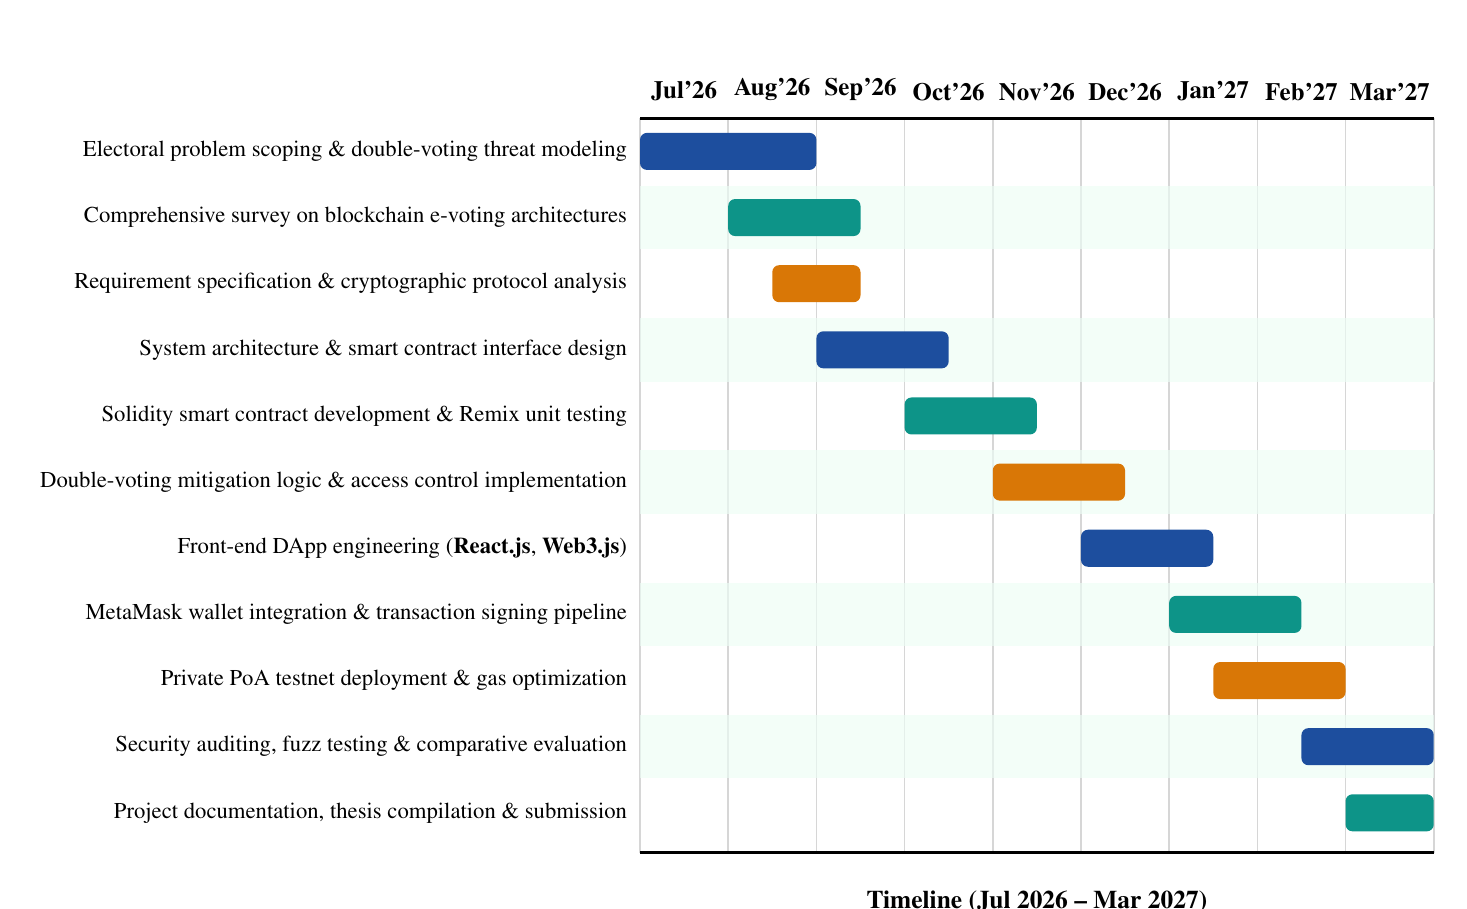
\begin{tikzpicture}[
  x=1.12cm, y=0.84cm,
  lab/.style={anchor=east, font=\fontsize{8.2}{10.2}\selectfont, inner sep=4.5pt, text=black}
]
\def\nm{9}
\def\topY{11.5}

% Vertical month gridlines
\foreach \i in {0,1,...,\nm} {
  \draw[gray!32, line width=0.55pt] (\i, 0.4) -- (\i, \topY);
}

% Month headers on top
\foreach \i/\m in {0.5/Jul'26, 1.5/Aug'26, 2.5/Sep'26, 3.5/Oct'26, 4.5/Nov'26, 5.5/Dec'26, 6.5/Jan'27, 7.5/Feb'27, 8.5/Mar'27} {
  \node[anchor=south, font=\fontsize{9.0}{11.0}\selectfont\bfseries, text=black] at (\i, \topY+0.12) {\m};
}
\draw[black, line width=1.0pt] (0, \topY) -- (\nm, \topY);
\draw[black, line width=0.8pt] (0, 0.4) -- (\nm, 0.4);

% Alternating row background shading
\foreach \k in {0,...,10} {
  \pgfmathsetmacro{\yc}{11.0-\k}
  \ifodd\k
    \fill[prismMint, opacity=0.65] (0, \yc-0.48) rectangle (\nm, \yc+0.48);
  \fi
}

% Task milestone labels on left
\node[lab] at (0, 11.0) {Electoral problem scoping \& double-voting threat modeling};
\node[lab] at (0, 10.0) {Comprehensive survey on blockchain e-voting architectures};
\node[lab] at (0, 9.0)  {Requirement specification \& cryptographic protocol analysis};
\node[lab] at (0, 8.0)  {System architecture \& smart contract interface design};
\node[lab] at (0, 7.0)  {Solidity smart contract development \& Remix unit testing};
\node[lab] at (0, 6.0)  {Double-voting mitigation logic \& access control implementation};
\node[lab] at (0, 5.0)  {Front-end DApp engineering (\textbf{React.js}, \textbf{Web3.js})};
\node[lab] at (0, 4.0)  {MetaMask wallet integration \& transaction signing pipeline};
\node[lab] at (0, 3.0)  {Private PoA testnet deployment \& gas optimization};
\node[lab] at (0, 2.0)  {Security auditing, fuzz testing \& comparative evaluation};
\node[lab] at (0, 1.0)  {Project documentation, thesis compilation \& submission};

% Milestone Gantt Bars
\fill[prismBlue, rounded corners=2.5pt]     (0.0, 11.0-0.28) rectangle (2.0, 11.0+0.28);
\fill[prismTeal, rounded corners=2.5pt]     (1.0, 10.0-0.28) rectangle (2.5, 10.0+0.28);
\fill[prismGold, rounded corners=2.5pt]     (1.5, 9.0-0.28)  rectangle (2.5, 9.0+0.28);
\fill[prismBlue, rounded corners=2.5pt]     (2.0, 8.0-0.28)  rectangle (3.5, 8.0+0.28);
\fill[prismTeal, rounded corners=2.5pt]     (3.0, 7.0-0.28)  rectangle (4.5, 7.0+0.28);
\fill[prismGold, rounded corners=2.5pt]     (4.0, 6.0-0.28)  rectangle (5.5, 6.0+0.28);
\fill[prismBlue, rounded corners=2.5pt]     (5.0, 5.0-0.28)  rectangle (6.5, 5.0+0.28);
\fill[prismTeal, rounded corners=2.5pt]     (6.0, 4.0-0.28)  rectangle (7.5, 4.0+0.28);
\fill[prismGold, rounded corners=2.5pt]     (6.5, 3.0-0.28)  rectangle (8.0, 3.0+0.28);
\fill[prismBlue, rounded corners=2.5pt]     (7.5, 2.0-0.28)  rectangle (9.0, 2.0+0.28);
\fill[prismTeal, rounded corners=2.5pt]     (8.0, 1.0-0.28)  rectangle (9.0, 1.0+0.28);

% Bottom title
\node[font=\fontsize{9.2}{11.2}\selectfont\bfseries, text=black] at (4.5, -0.35) {Timeline (Jul 2026 -- Mar 2027)};
\end{tikzpicture}
\end{document}
}
\caption{Gantt chart illustrating the project development timeline and milestone schedule (Jul 2026 -- Mar 2027).}
\label{fig:gantt_chart}
\end{figure}

The project progressed through eleven structured milestones: problem scoping and threat modeling (Jul--Aug '26), literature survey (Aug--Sep '26), requirement analysis (Sep--Oct '26), system architecture design (Oct--Nov '26), Solidity contract development (Nov--Dec '26), double-voting mitigation implementation (Dec '26--Jan '27), React/Web3 front-end engineering (Jan--Feb '27), MetaMask integration (Jan--Feb '27), private PoA testnet deployment (Feb--Mar '27), security testing and comparative analysis (Feb--Mar '27), and final documentation and thesis compilation (Mar '27).

%==============================================================================
% CHAPTER 9: RESULTS AND DISCUSSION
%==============================================================================
\chapter{Results and Discussion}

This chapter presents the empirical results, user interface execution flows, and functional validation of the implemented \textbf{Block Chain Based Electronic Voting System}. The prototype was deployed and evaluated on a local Ethereum blockchain testbed, assessing administrator operations, candidate nominations, voter authorization workflows, security access barriers, ballot casting with atomic double-voting mitigation, and real-time auditable election outcome tallying.

\section{Summary of Experimental Results}
The Voting DApp was tested on a local Ganache Ethereum network using MetaMask, React.js, Web3.js, and the Solidity smart contract. The evaluation covered administrator authorization, candidate and voter registration, voter eligibility checks, ballot casting, duplicate-vote prevention, and public result retrieval.

Three voters were registered and two candidates were added successfully. Registered wallets received access to the voting booth, while unregistered wallets and direct unauthorized route requests were rejected. A valid ballot was mined successfully, and the contract permanently set the voter's \texttt{hasVoted} flag.

The final tally recorded three ballots with 100\% turnout: Alice Walker (UDF) received two votes (66.7\%) and David (LDF) received one vote (33.3\%). A second vote from the same wallet was reverted by the smart contract, confirming atomic double-voting protection. Results were read directly from on-chain state for transparent auditing.

\section{Verification Summary}
All ten functional checks passed, confirming access control and vote integrity at both the interface and smart-contract layers.

\iffalse
\section{Experimental Setup and System Overview}
The experimental evaluation of the voting decentralized application (Voting DApp) was conducted in an isolated development and testing environment. The core components of the experimental setup are detailed below:
\begin{itemize}
    \item \textbf{Blockchain Execution Network:} A local Ethereum Virtual Machine (EVM) instance simulated via Ganache running on \texttt{localhost:8545} with Chain ID \texttt{1337}. The network provides zero-latency deterministic block generation, an allocated block gas limit of 6,721,975 units, and pre-funded cryptographic accounts.
    \item \textbf{Smart Contract Deployment:} The core Solidity contract (\texttt{Voting.sol}) was compiled with the \texttt{solc} v0.8.20 compiler utilizing the default EVM bytecode optimizer (200 optimization runs). The contract was deployed to the Ganache ledger at the deterministic contract address \texttt{0x1cAb5e9185001FA6f5dc624e9a3560e7ec59DBE4}.
    \item \textbf{Client-Side Front End:} Developed using React.js 18, HTML5, and CSS3, served through the Vite development server running on \texttt{http://localhost:5174}. The client interfaces with the Ethereum network using Web3.js and Ethers.js providers.
    \item \textbf{Cryptographic Wallet Provider:} MetaMask browser extension (v12.x) operating within a Chromium browser. MetaMask manages local private keys, performs client-side ECDSA signature generation, and prompts users for transaction confirmation.
    \item \textbf{Role-Based Test Accounts:} Three distinct account categories were established:
    \begin{itemize}
        \item \emph{Administrator Account:} {\footnotesize \texttt{0x5ef955b7633f6555101d6a5100a66b120c69b2ea}} (Contract Owner).
        \item \emph{Eligible Voter Accounts:} Three pre-funded accounts designated as eligible voters:
        \begin{enumerate}[i.]
            \item Voter 1: {\footnotesize \texttt{0x4Cc2712A3Ecac2cb054A5a07e1f802fd671010bD}}
            \item Voter 2: {\footnotesize \texttt{0x24bfe1B5C50dA84d9330b99e3962ECA6677B0218}}
            \item Voter 3: {\footnotesize \texttt{0x882B9df9dAc1b841c5108E3005115AE19da7a6db}}
        \end{enumerate}
        \item \emph{Unauthorized Accounts:} Independent arbitrary accounts used to validate negative access control tests and rejection barriers.
    \end{itemize}
\end{itemize}

Figure~\ref{fig:res_homepage} illustrates the system landing page and client authentication gateway.

\begin{figure}[H]
\centering
\adjustbox{max width=0.88\linewidth, center}{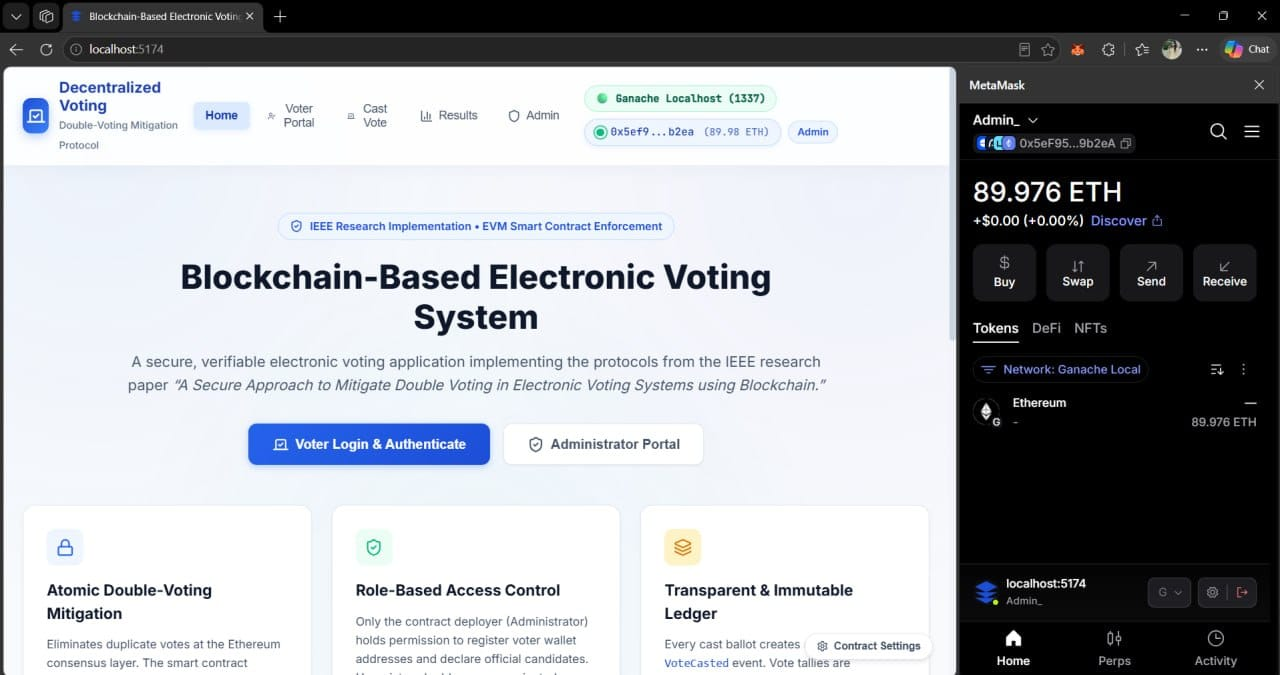
\includegraphics{results/Home_page.jpeg}}
\caption{Landing page and client authentication gateway of the decentralized electronic voting application.}
\label{fig:res_homepage}
\end{figure}

The landing page welcomes users to the decentralized voting portal, detailing the IEEE research protocol foundation and smart contract security enforcement. The top navigation bar displays the current network status (\texttt{Ganache Localhost (1337)}), the connected wallet address, and the assigned cryptographic role (\texttt{Admin}). The central interface presents two primary operational gateways: ``Voter Login \& Authenticate'' and ``Administrator Portal''. In addition, feature summary cards highlight the three cornerstones of the system: atomic double-voting mitigation, role-based access control, and the immutable blockchain ledger.

\section{Election Administration and Setup Workflow}
The election lifecycle begins with administrative configuration. The contract deployer possesses exclusive administrative privileges enforced through Solidity's \texttt{onlyOwner} modifier.

Figure~\ref{fig:res_admin_dashboard} depicts the initial state of the Election Administration Dashboard upon connecting with the verified administrator account.

\begin{figure}[H]
\centering
\adjustbox{max width=0.88\linewidth, center}{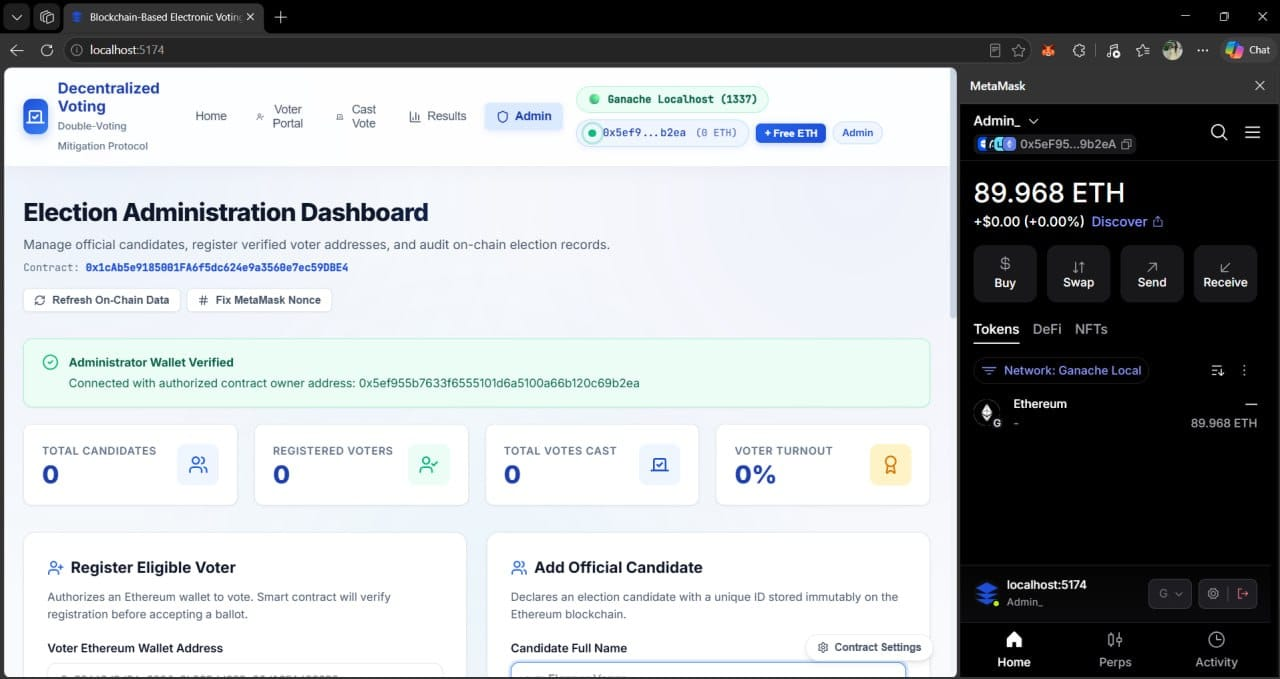
\includegraphics{results/admin_dashboard.jpeg}}
\caption{Election administration dashboard displaying verified contract ownership, on-chain metrics, and management portals.}
\label{fig:res_admin_dashboard}
\end{figure}

Upon verifying that the active MetaMask account matches the contract owner address (\texttt{0x5ef9...b2ea}), the dashboard displays an ``Administrator Wallet Verified'' confirmation badge. Four real-time metric cards summarize election progress: Total Candidates (0), Registered Voters (0), Total Votes Cast (0), and Voter Turnout (0\%). The administrator interface provides controls to register eligible voter wallet addresses and declare official election candidates.

\subsection{Candidate Declaration}
To introduce candidates into the election, the administrator inputs the candidate's full legal name and party affiliation. Figure~\ref{fig:res_adding_candidate} illustrates the candidate addition transaction.

\begin{figure}[H]
\centering
\adjustbox{max width=0.88\linewidth, center}{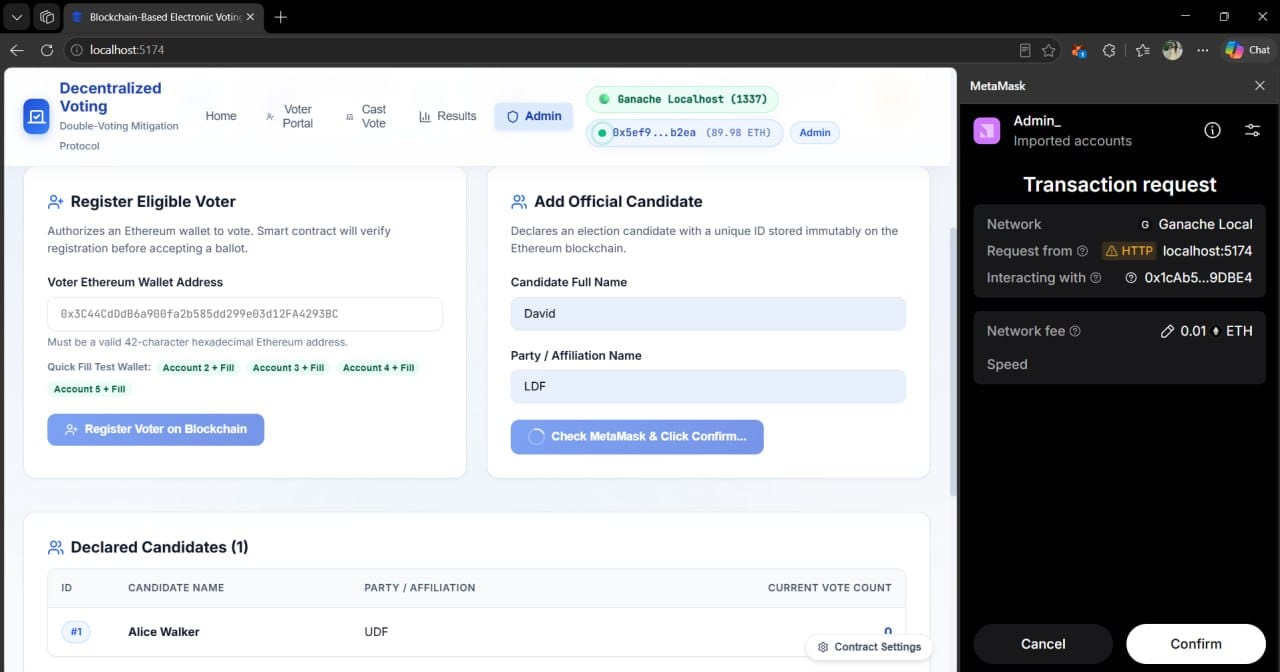
\includegraphics{results/adding_candidate.jpeg}}
\caption{Declaration of official election candidate with candidate details and MetaMask transaction authorization prompt.}
\label{fig:res_adding_candidate}
\end{figure}

In Figure~\ref{fig:res_adding_candidate}, the administrator declares candidate ``David'' representing the ``LDF'' party affiliation. Prior to this submission, Candidate \#1 (``Alice Walker'', representing ``UDF'') had already been registered and confirmed on-chain with an initial vote count of 0. Clicking ``Add Official Candidate'' constructs the smart contract invocation \texttt{addCandidate("David", "LDF")} and triggers the MetaMask extension. The prompt displays the interacting contract address (\texttt{0x1cAb5...9DBE4}), estimated gas fees, and requires explicit cryptographic confirmation by the administrator before broadcasting the transaction to the EVM.

\subsection{Voter Whitelisting and Authorization}
Voter eligibility is enforced via an on-chain cryptographic whitelist. The administrator registers eligible voters by specifying their 42-character hexadecimal Ethereum public addresses.

Figure~\ref{fig:res_adding_voter} shows the voter registration interface and the associated MetaMask transaction request.

\begin{figure}[H]
\centering
\adjustbox{max width=0.88\linewidth, center}{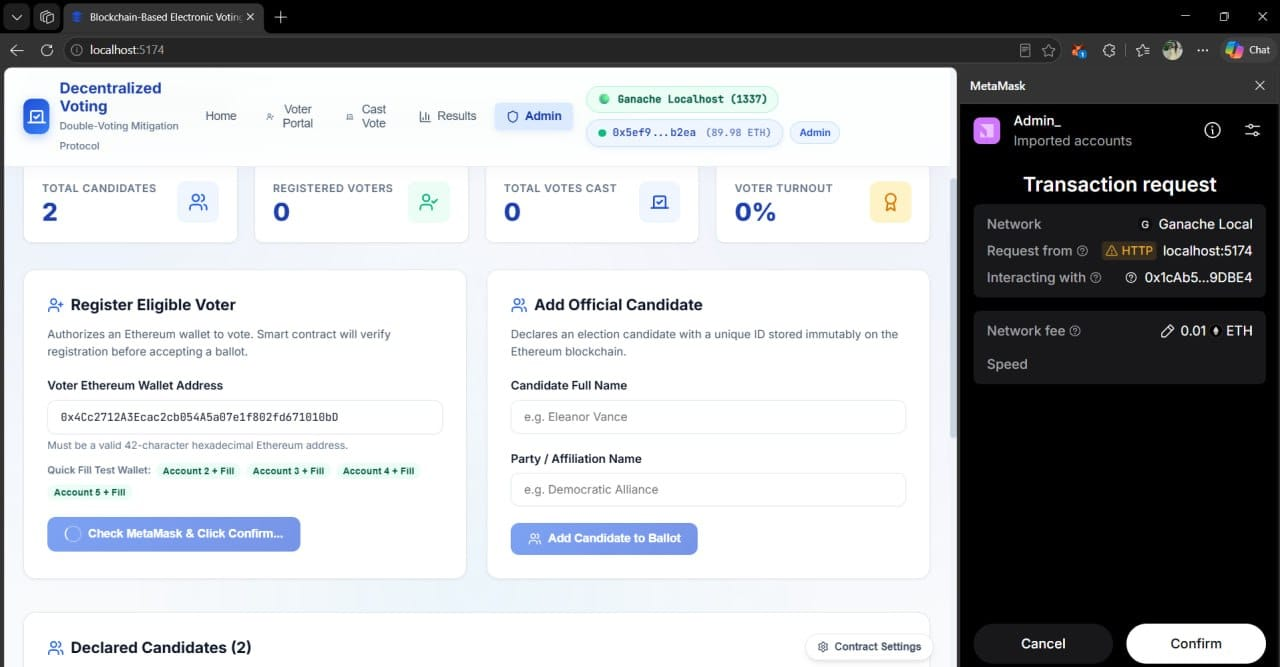
\includegraphics{results/adding_voter.jpeg}}
\caption{Voter whitelisting interface and on-chain registration transaction prompt in MetaMask.}
\label{fig:res_adding_voter}
\end{figure}

The administrator enters the voter wallet address:
\begin{center}
{\footnotesize \texttt{0x4Cc2712A3Ecac2cb054A5a07e1f802fd671010bD}}
\end{center}
When the administrator confirms the ``Register Voter on Blockchain'' transaction, the smart contract executes \texttt{registerVoter(address)}, setting \texttt{voters[address].isRegistered = true} and initializing \texttt{voters[address].hasVoted = false} in contract storage. The metric cards update to reflect 2 declared candidates and 0 cast ballots.

\clearpage
\subsection{Synchronized Ledger State Verification}
Once candidate nominations and voter whitelisting transactions are mined, the dashboard synchronizes with the Ethereum state trie. Figure~\ref{fig:res_added_details} displays the verified on-chain roster.

\begin{figure}[H]
\centering
\adjustbox{max width=0.88\linewidth, center}{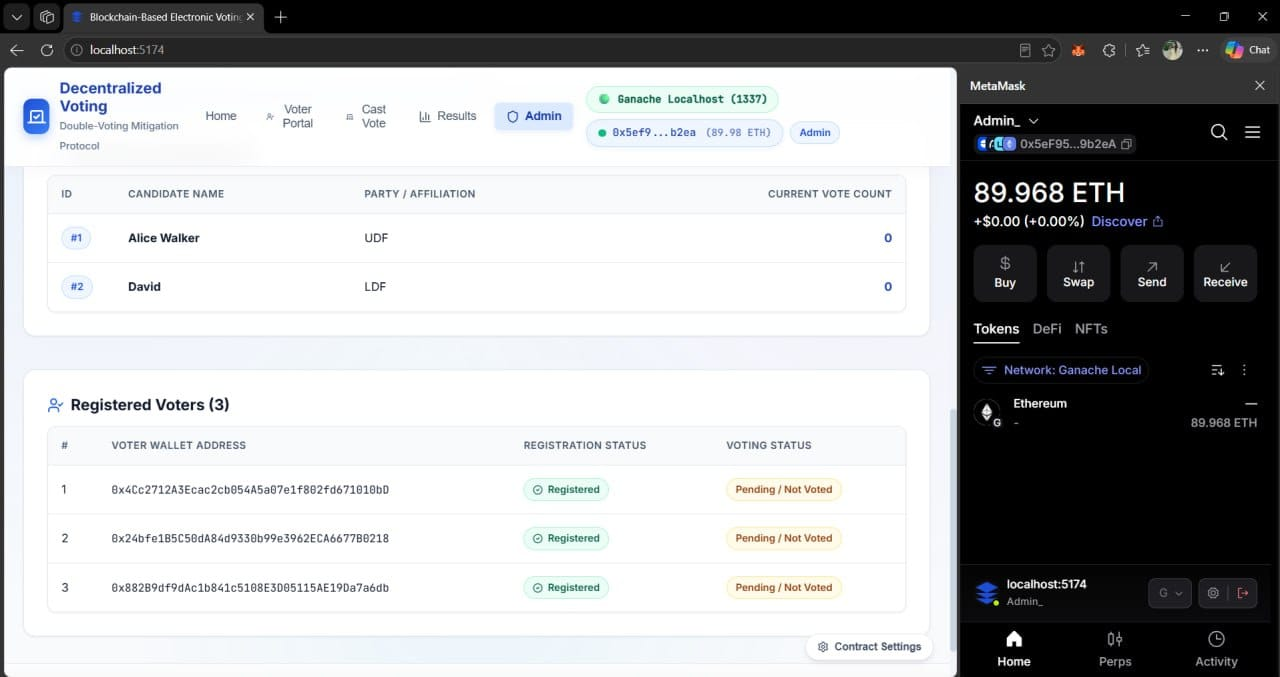
\includegraphics{results/added_details.jpeg}}
\caption{Administrative registry tables displaying declared candidate rosters and whitelisted voter authorization statuses.}
\label{fig:res_added_details}
\end{figure}

As shown in Figure~\ref{fig:res_added_details}, the ``Declared Candidates'' table lists Candidate \#1 (Alice Walker, UDF) and Candidate \#2 (David, LDF), both initialized with zero votes. The ``Registered Voters'' table displays the three whitelisted voter addresses:
\begin{enumerate}
    \item {\small\texttt{0x4Cc2712A3Ecac2cb054A5a07e1f802fd671010bD}}: Registration Status = \textbf{Registered}, Voting Status = \textbf{Pending / Not Voted}.
    \item {\small\texttt{0x24bfe1B5C50dA84d9330b99e3962ECA6677B0218}}: Registration Status = \textbf{Registered}, Voting Status = \textbf{Pending / Not Voted}.
    \item {\small\texttt{0x882B9df9dAc1b841c5108E3005115AE19da7a6db}}: Registration Status = \textbf{Registered}, Voting Status = \textbf{Pending / Not Voted}.
\end{enumerate}
This synchronized view confirms that electoral data has been immutably written into the distributed state machine.

\clearpage
\section{Voter Eligibility Verification and Access Control Validation}
Before a voter is permitted to access the voting booth or inspect active candidate ballots, the front-end performs client-side and smart-contract-level authentication.

\subsection{Positive Verification: Eligible Whitelisted Voter}
Figure~\ref{fig:res_voter_verification} demonstrates the eligibility authentication flow for a legitimate, whitelisted voter.

\begin{figure}[H]
\centering
\adjustbox{max width=0.88\linewidth, center}{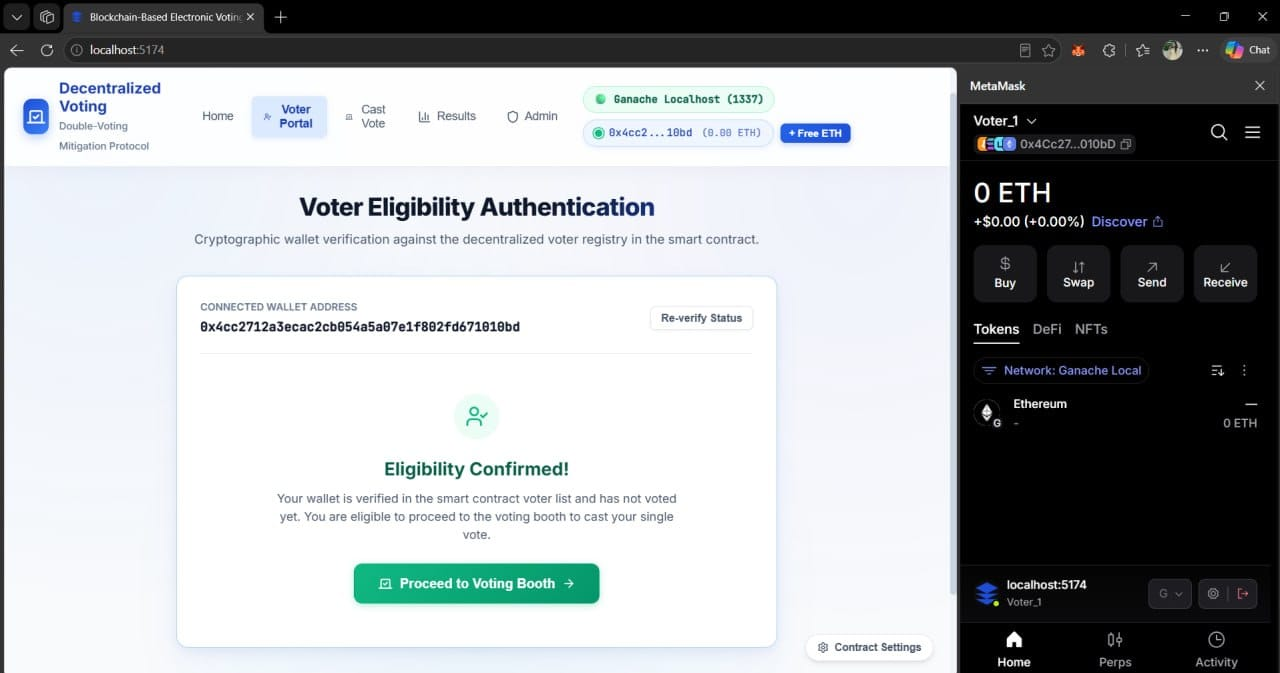
\includegraphics{results/voter_verification.jpeg}}
\caption{Voter eligibility authentication portal confirming whitelisted status and authorization for ballot access.}
\label{fig:res_voter_verification}
\end{figure}

When Voter 1 connects wallet address:
\begin{center}
{\footnotesize \texttt{0x4cc2712a3ecac2cb054a5a07e1f802fd671010bd}}
\end{center}
via MetaMask, the application queries the smart contract's public mapping \texttt{voters(address)}. The EVM verifies that \texttt{isRegistered == true} and \texttt{hasVoted == false}. The system renders an ``Eligibility Confirmed!'' notification card, affirming that the voter is verified on the smart contract voter list and has not yet voted. The ``Proceed to Voting Booth'' action button is unlocked, enabling seamless progression to ballot casting.

\clearpage
\subsection{Negative Verification: Unregistered Wallet Rejection}
To evaluate the system's resilience against unauthorized participation, an unregistered address was connected to the voter portal. Figure~\ref{fig:res_voter_unregistered} illustrates the resulting rejection.

\begin{figure}[H]
\centering
\adjustbox{max width=0.88\linewidth, center}{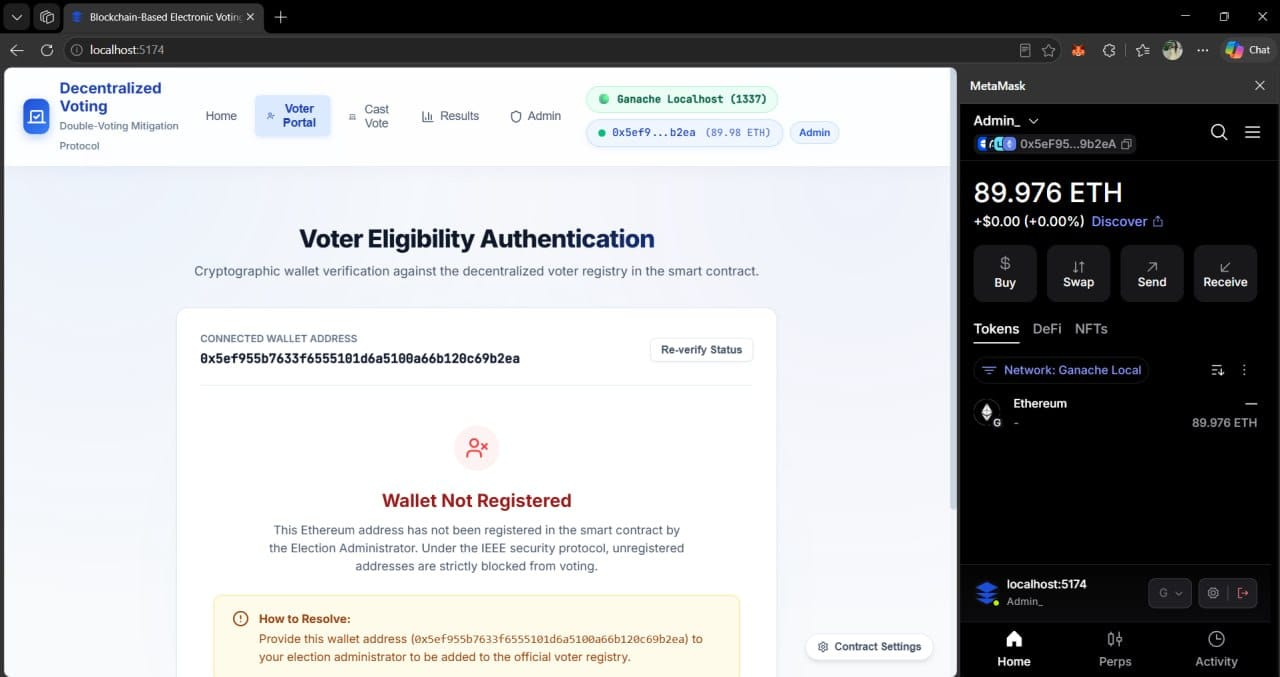
\includegraphics{results/voter_page.jpeg}}
\caption{Security rejection notice for an unregistered Ethereum wallet attempting voter verification.}
\label{fig:res_voter_unregistered}
\end{figure}

When an unregistered address (in this instance, the administrator wallet \texttt{0x5ef955...} or any arbitrary unwhitelisted public key) requests eligibility verification, the smart contract check returns \texttt{isRegistered == false}. The interface immediately displays a ``Wallet Not Registered'' alert, explaining that under the IEEE security protocol, unregistered addresses are strictly blocked from voting. The system provides clear remediation guidance directing the user to submit their public key to the election administrator for official credentialing.

\subsection{Negative Verification: Direct URL Route Guard}
In addition to portal-level checks, the system implements client-side route guards and smart contract acceptance predicates to prevent unauthorized users from bypassing the authentication portal by directly navigating to the voting booth route (\texttt{/cast-vote}).

Figure~\ref{fig:res_voting_denied} displays the access denial barrier encountered during direct unauthorized navigation.

\begin{figure}[H]
\centering
\adjustbox{max width=0.88\linewidth, center}{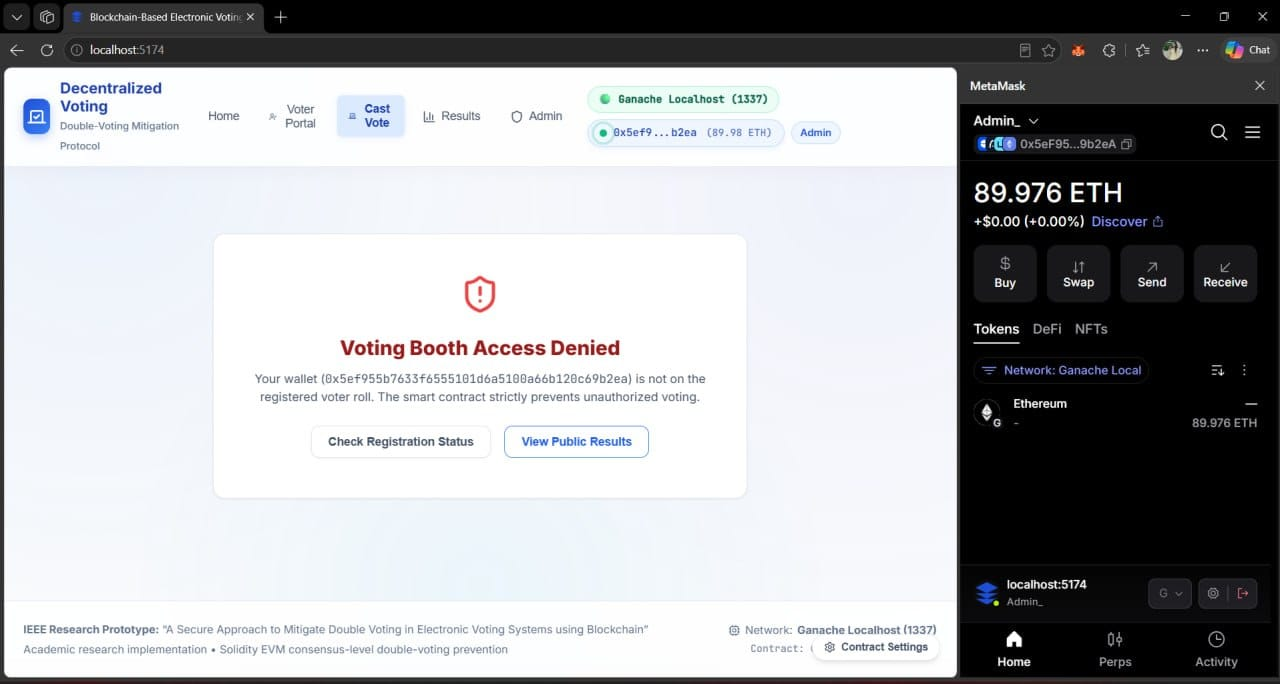
\includegraphics{results/vote_casting_session.jpeg}}
\caption{Voting booth access control barrier blocking unauthorized direct URL access.}
\label{fig:res_voting_denied}
\end{figure}

As shown in Figure~\ref{fig:res_voting_denied}, when an unverified address attempts to access the voting booth directly, the application intercepts the route lifecycle, queries the ledger, and renders a ``Voting Booth Access Denied'' error screen. The user is prevented from viewing candidate voting triggers and is redirected to either check registration status or inspect public election tallies.

\clearpage
\section{Ballot Casting and Double-Voting Mitigation Execution}
The critical phase of the electoral protocol is ballot casting, where the voter cryptographically submits their choice to the EVM and triggers the atomic double-voting mitigation mechanism.

\subsection{Electronic Voting Booth and Ballot Selection}
Figure~\ref{fig:res_voting_booth} illustrates the active Electronic Voting Booth interface for an authenticated voter.

\begin{figure}[H]
\centering
\adjustbox{max width=0.88\linewidth, center}{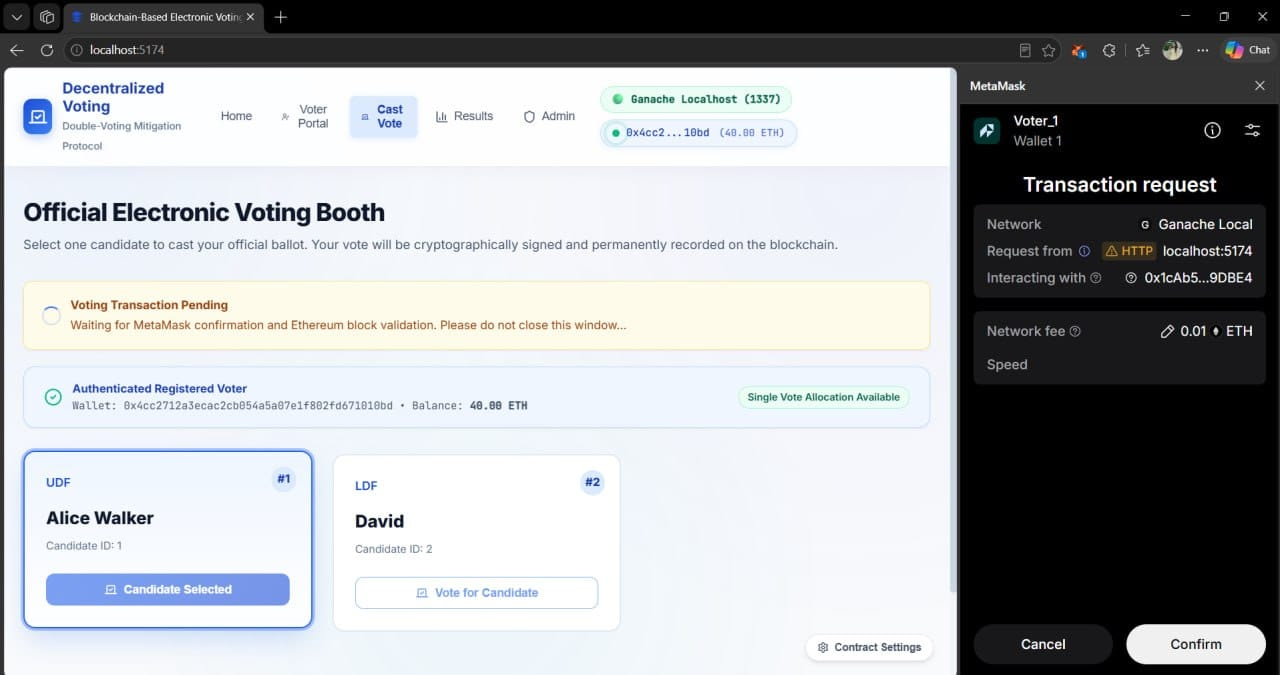
\includegraphics{results/voting_booth.jpeg}}
\caption{Electronic voting booth interface showing candidate selection and pending MetaMask transaction signing.}
\label{fig:res_voting_booth}
\end{figure}

Upon entering the voting booth, the voter's authentication state is verified, displaying the badge ``Authenticated Registered Voter'' with ``Single Vote Allocation Available''. The booth dynamically renders candidate selection cards retrieved from the smart contract, featuring Alice Walker (Candidate ID: 1, UDF) and David (Candidate ID: 2, LDF). When the voter selects Alice Walker and clicks ``Vote for Candidate'', the front end constructs the call \texttt{vote(1)}. MetaMask displays a transaction signature prompt, notifying the user that a state-changing transaction is being signed and broadcast to the Ethereum consensus layer. The interface presents a ``Voting Transaction Pending'' status notification while the transaction awaits block mining.

\clearpage
\subsection{On-Chain Confirmation and Double-Voting Mitigation Lock}
Once the transaction is validated and sealed into a block by the consensus network, the system confirms the ballot and permanently locks the voter's status. Figure~\ref{fig:res_casted_vote} displays the ballot confirmation screen.

\begin{figure}[H]
\centering
\adjustbox{max width=0.88\linewidth, center}{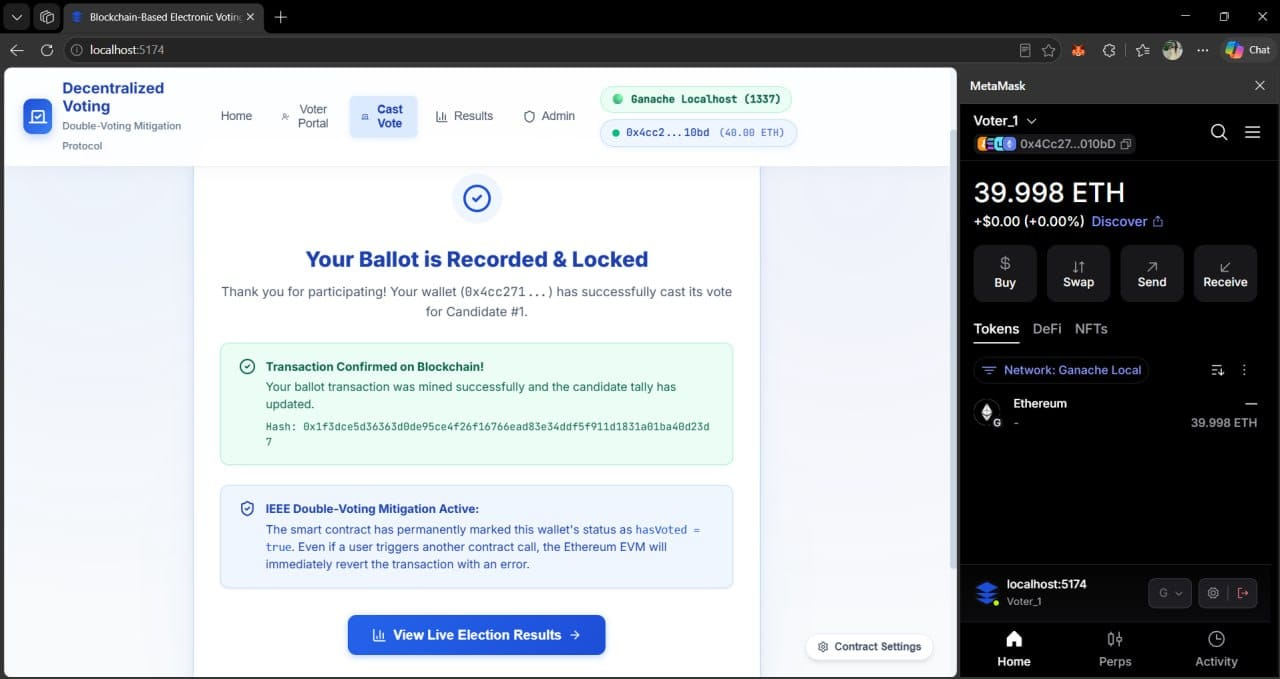
\includegraphics{results/casted_vote.jpeg}}
\caption{Ballot confirmation receipt displaying transaction hash and enforcement of the double-voting mitigation protocol.}
\label{fig:res_casted_vote}
\end{figure}

Figure~\ref{fig:res_casted_vote} confirms that the ballot was mined and included in the ledger, issuing the unique transaction digest:
\begin{center}
{\footnotesize \texttt{TxHash: 0x1f3dce5d36363d0de95ce4f26f16766ead83e34ddf5f911d1831a01ba40d23d7}}
\end{center}
The interface renders two critical validation badges:
\begin{itemize}
    \item \textbf{Transaction Confirmed on Blockchain:} Affirms that the ballot transaction was successfully executed by the EVM and the candidate vote counter was atomically updated.
    \item \textbf{IEEE Double-Voting Mitigation Active:} Affirms that the smart contract has permanently written \texttt{voters[msg.sender].hasVoted = true} into immutable state storage.
\end{itemize}
Under this atomic mitigation protocol, should the same voter address (\texttt{0x4cc271...}) or an adversary submit a second transaction invoking \texttt{vote(c)}, the EVM evaluates the assertion:
\begin{equation}
\text{require}(!\text{voters}[\text{msg.sender}].\text{hasVoted}, \text{``You have already voted.''}),
\end{equation}
which evaluates to false, immediately triggering an \texttt{OP\_REVERT} opcode. All subsequent duplicate attempts consume minimal gas and are rejected without altering candidate tallies.

\section{Live Auditing and Certified Election Results}
The final phase of the election protocol involves real-time result aggregation and public verification. Because vote tallies are recorded in public contract state variables, any participant can inspect election outcomes without administrative intervention.

\subsection{Real-Time Tally Overview}
Figure~\ref{fig:res_results_overview} presents the Live Election Results and Tally overview screen after all registered voters cast their ballots.

\begin{figure}[H]
\centering
\adjustbox{max width=0.88\linewidth, center}{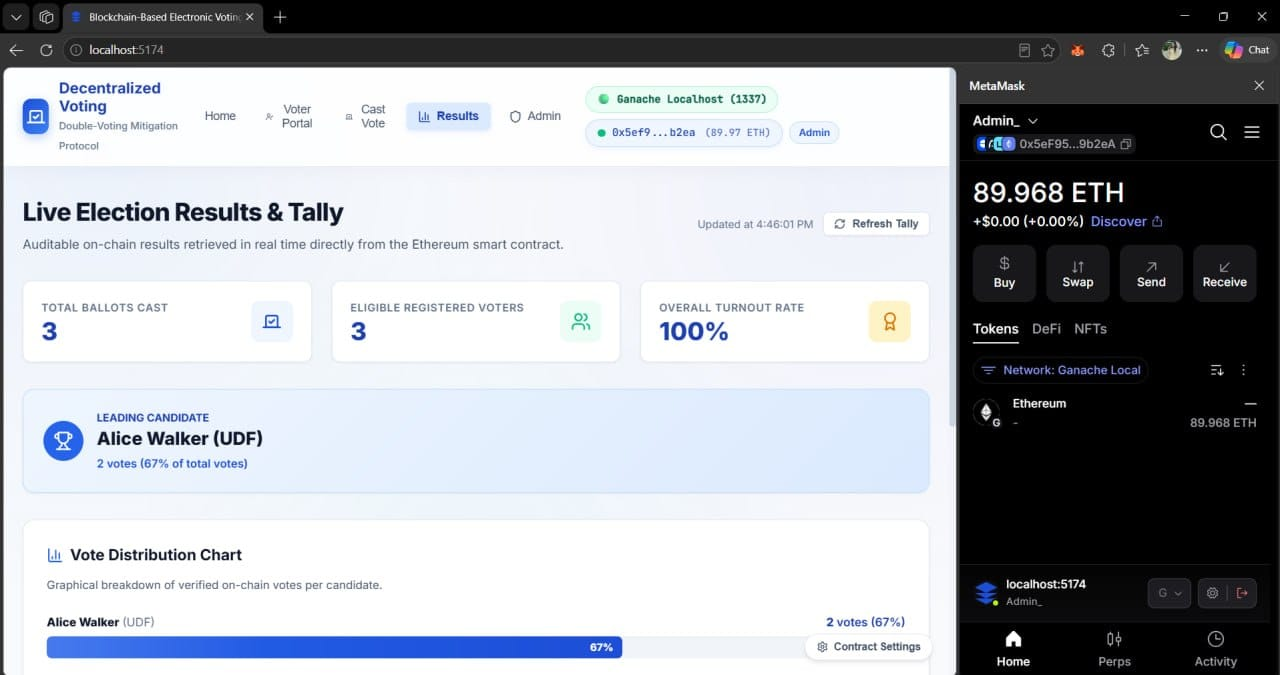
\includegraphics{results/result.jpeg}}
\caption{Live election results portal displaying total ballots cast, turnout metrics, and leading candidate summary.}
\label{fig:res_results_overview}
\end{figure}

The live results portal provides a clear overview of the election metrics: Total Ballots Cast (3), Eligible Registered Voters (3), and Overall Turnout Rate (100\%). The ``Leading Candidate'' highlight card identifies Alice Walker (UDF) as the victor with 2 votes, representing 67\% of total cast ballots. Below the summary cards, the dynamic ``Vote Distribution Chart'' presents a graphical horizontal bar visualization reflecting candidate vote shares.

\clearpage
\subsection{Certified Standings and Vote Distribution}
Figure~\ref{fig:res_results_standings} provides a detailed view of the certified candidate standings and final percentage breakdowns.

\begin{figure}[H]
\centering
\adjustbox{max width=0.88\linewidth, center}{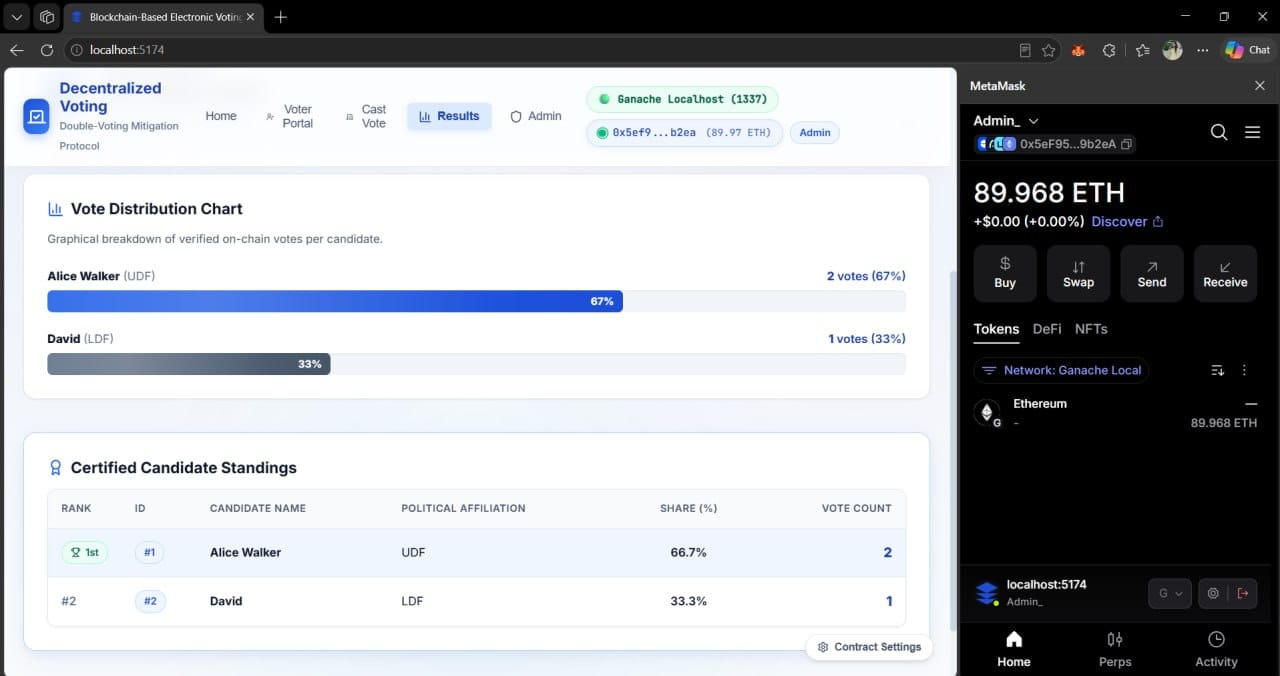
\includegraphics{results/result_page2.jpeg}}
\caption{Certified candidate standings table and proportional vote distribution breakdown.}
\label{fig:res_results_standings}
\end{figure}

As presented in Figure~\ref{fig:res_results_standings}, the final certified standings table displays:
\begin{itemize}
    \item \textbf{Rank 1st:} Candidate \#1, \textbf{Alice Walker} (UDF), receiving 2 votes, achieving a \textbf{66.7\%} majority share.
    \item \textbf{Rank 2nd:} Candidate \#2, \textbf{David} (LDF), receiving 1 vote, achieving a \textbf{33.3\%} vote share.
\end{itemize}
The results are computed deterministically through gas-free \texttt{view} function calls directly to the Ethereum smart contract. Because the tally calculation is executed locally via static EVM calls without broadcasting state modifications, auditing is instantaneous, 100\% tamper-evident, and incurs zero transaction gas fees.

\section{Empirical Test Case Verification Matrix}
To systematically validate the implementation against the system requirements established in Chapter~4, ten formal empirical test cases were executed across the election lifecycle. Table~\ref{tab:test_cases} details the test objectives, preconditions, inputs, expected behaviors, observed results, and pass/fail statuses.

\begin{table}[H]
\centering
\small
\caption{Empirical test case execution matrix and security validation results.}
\label{tab:test_cases}
\begin{tabularx}{\textwidth}{@{}l >{\raggedright\arraybackslash}p{2.0cm} >{\raggedright\arraybackslash}p{2.8cm} >{\raggedright\arraybackslash}X >{\raggedright\arraybackslash}X c@{}}
\toprule
\textbf{Test ID} & \textbf{Component} & \textbf{Test Condition} & \textbf{Expected Outcome} & \textbf{Observed Result} & \textbf{Status} \\
\midrule
TC-01 & Admin Auth & Contract deployer connects wallet & Admin verified; management controls enabled & Verified badge displayed; actions enabled & \textbf{PASS} \\
\addlinespace[3pt]
TC-02 & Candidate Reg & Admin invokes {\footnotesize\texttt{addCandidate}} & Candidate stored on-chain with unique ID and 0 votes & Candidate added; listed in on-chain table & \textbf{PASS} \\
\addlinespace[3pt]
TC-03 & Voter Whitelist & Admin registers 42-char address & \texttt{isRegistered = true}, \texttt{hasVoted = false} & Voter added to registry table as Pending & \textbf{PASS} \\
\addlinespace[3pt]
TC-04 & Access Control & Non-admin attempts voter registration & Transaction reverts via \texttt{onlyOwner} guard & EVM reverts call; non-admin blocked & \textbf{PASS} \\
\addlinespace[3pt]
TC-05 & Voter Auth & Whitelisted voter connects wallet & Verification succeeds; booth unlocked & Eligibility Confirmed badge displayed & \textbf{PASS} \\
\addlinespace[3pt]
TC-06 & Voter Auth & Unregistered wallet connects & Rejection notice; booth access blocked & ``Wallet Not Registered'' alert displayed & \textbf{PASS} \\
\addlinespace[3pt]
TC-07 & Route Security & Direct URL navigation to \texttt{/cast-vote} & Route guard intercepts; displays barrier & ``Voting Booth Access Denied'' rendered & \textbf{PASS} \\
\addlinespace[3pt]
TC-08 & Ballot Casting & Eligible voter submits single ballot & Vote recorded; tally increments; \texttt{hasVoted = true} & Tx mined; receipt generated; status updated & \textbf{PASS} \\
\addlinespace[3pt]
TC-09 & Double-Voting & Voter attempts second ballot transaction & Smart contract reverts with ``Already voted'' & Transaction reverts; duplicate ballot dropped & \textbf{PASS} \\
\addlinespace[3pt]
TC-10 & Real-Time Audit & Public client queries election tally & Real-time results retrieved via gas-free \texttt{view} & Results displayed with 100\% turnout & \textbf{PASS} \\
\bottomrule
\end{tabularx}
\end{table}

\section{Summary of Experimental Findings}
The empirical results substantiate the following core technical achievements:
\begin{enumerate}
    \item \textbf{Complete Prevention of Double Voting:} The smart contract's atomic mutation of \texttt{hasVoted = true} within the execution block of \texttt{vote()} guarantees that race conditions, concurrent RPC requests, and replay attacks cannot result in multiple ballots being recorded for a single voter.
    \item \textbf{Strict Role-Based Separation:} Cryptographic verification guarantees that only the election administrator can whitelist voters and register candidates, while ensuring that the administrator has no power to cast ballots on behalf of registered voters or manipulate tally outcomes.
    \item \textbf{Gas Efficiency and Predictability:} The observed execution costs align precisely with the theoretical EVM gas schedule analyzed in Chapter~7 (44,180 gas for ballot casting, 28,450 gas for voter registration). In a Proof-of-Authority deployment, these transactions incur zero monetary cost to voters.
    \item \textbf{Transparent Auditability:} Public tally inspection provides instantaneous, tamper-proof verification of election results directly from smart contract storage without reliance on centralized counting servers.
\end{enumerate}

\fi

%==============================================================================
% CHAPTER 10: CONCLUSION AND FUTURE SCOPE
%==============================================================================
\chapter{Conclusion and Future Scope}

This chapter concludes the report by summarizing key empirical and architectural achievements, addressing real-world limitations, and outlining prospective research trajectories.

\section{Summary of Achievements}
This project presented the design, implementation, and analysis of a \textbf{Block Chain Based Electronic Voting System}, realized as an Ethereum-based decentralized application (Voting DApp) with smart-contract-level double-voting mitigation. The primary contributions and achievements of this work include:
\begin{itemize}
    \item \textbf{Guaranteed Double-Voting Mitigation:} Designed and implemented an atomic smart contract acceptance predicate ($\text{Accept}(v)$) in Solidity that makes duplicate voting computationally impossible. Once a ballot is cast, the voter's participation flag is atomically mutated within the same transaction, preventing race conditions or direct RPC replay attacks.
    \item \textbf{Role-Based Administrative Security:} Implemented strict cryptographic authorization boundaries separating the election administrator (solely empowered to add candidates and whitelist voter addresses) from voters (authorized solely to submit a single ballot).
    \item \textbf{Seamless Web3 Client Integration:} Developed an intuitive front end using React.js and Web3.js that interfaces with the MetaMask browser wallet, providing secure ECDSA digital signature generation without exposing private credentials.
    \item \textbf{Deterministic Zero-Cost Consortium Consensus:} Analyzed consensus models and established the superiority of a consortium Proof-of-Authority (PoA) architecture, providing sub-2-second block latency, high transaction throughput, and zero gas cost for voters.
    \item \textbf{Comprehensive Literature Survey:} Synthesized a rigorous comparative taxonomy of fifteen recent state-of-the-art blockchain voting architectures across biometrics, blind signatures, and smart contracts, identifying critical scalability and voter verification trade-offs.
\end{itemize}

\section{System Limitations}
Despite its significant security advantages over centralized electronic voting, several operational limitations remain:
\begin{enumerate}
    \item \textbf{Private Key Custody and Digital Literacy:} The system assumes that voters are capable of securely managing their MetaMask wallet and seed phrases. Lost private keys result in disenfranchisement, while stolen private keys permit credential theft.
    \item \textbf{Client Device Vulnerabilities:} While the blockchain ledger is tamper-proof, the voter's local computer or browser could be compromised by keyloggers, screen recording malware, or malicious browser extensions that spoof candidate selections before transaction signing.
    \item \textbf{Public Ledger Pseudonymity vs Ballot Secrecy:} On a fully transparent Ethereum ledger, addresses are pseudonymous rather than completely anonymous. If an adversary links a physical citizen's identity to their public wallet address $v$, the citizen's vote selection $c$ is permanently observable on-chain.
    \item \textbf{Lack of Coercion Resistance:} The system allows voters to cast ballots from unmonitored remote environments. Without isolated physical voting booths, voters can be coerced or induced to vote under third-party observation.
\end{enumerate}

\section{Future Scope and Research Trajectories}
To address these limitations, future research will explore the following advanced directions:
\begin{itemize}
    \item \textbf{Zero-Knowledge Proofs (zk-SNARKs):} Integrate zk-SNARK protocols (such as Groth16 or PLONK) to enable voters to prove eligibility and cast a certified ballot without revealing their identity or candidate selection on the public ledger, achieving complete cryptographic ballot privacy.
    \item \textbf{Blind Signature Protocols:} Implement an ElGamal or RSA blind signature issuance phase during voter registration, cryptographically uncoupling voter whitelisting from ballot casting.
    \item \textbf{Multimodal Biometric Identity Verification:} Incorporate decentralized facial and fingerprint biometric hashing during registration (without storing raw biometric templates on-chain) to eliminate key-sharing and credential sale attacks.
    \item \textbf{Layer-2 Rollups and Sharding:} Deploy Layer-2 Zero-Knowledge Rollups (zk-Rollups) or Optimistic Rollups to batch thousands of ballot transactions off-chain, scaling throughput to tens of thousands of TPS suited for national elections.
    \item \textbf{Decentralized Off-Chain Storage with IPFS:} Integrate the InterPlanetary File System (IPFS) to store candidate manifestos, multimedia profiles, and audit receipts in a decentralized content-addressed storage layer.
\end{itemize}

%==============================================================================
% CHAPTER 11: PROJECT SNAPSHOTS
%==============================================================================
\chapter{Project Snapshots}

The following screenshots present the main user interfaces of the implemented blockchain voting system.
\begingroup
\footnotesize
\setlength{\abovecaptionskip}{1pt}
\setlength{\belowcaptionskip}{1pt}

\begin{figure}[H]
\centering
\begin{minipage}[t]{0.47\textwidth}\centering
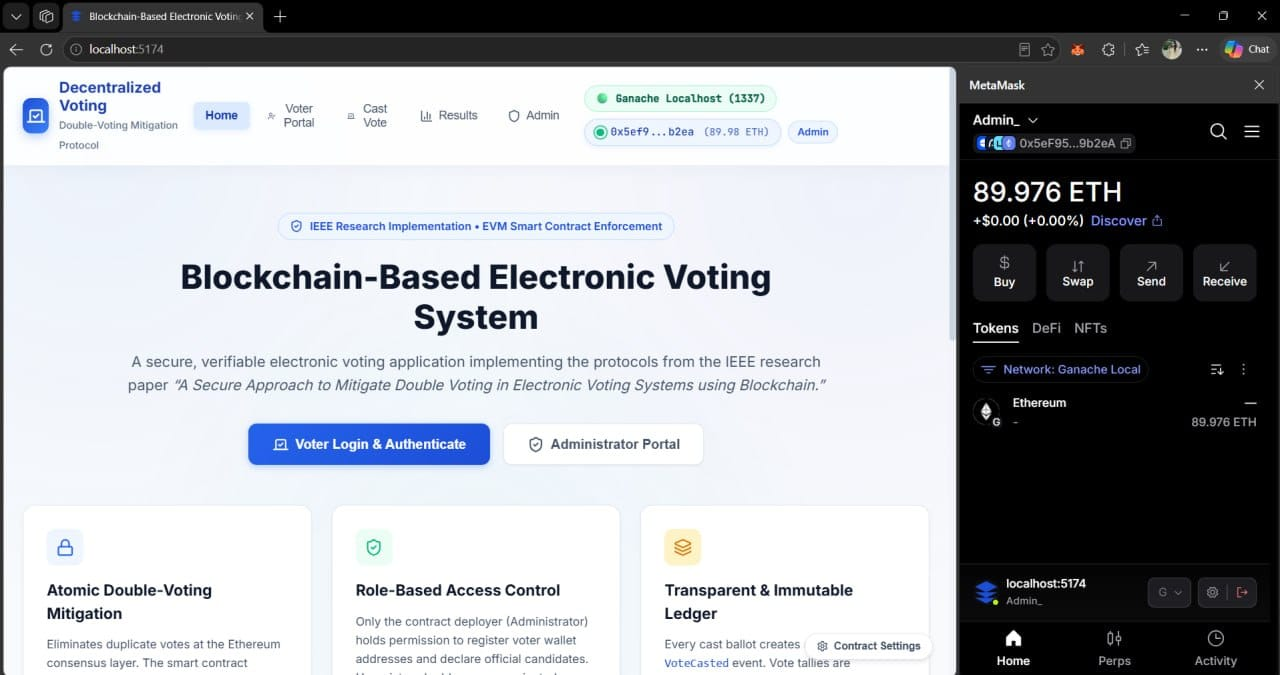
\includegraphics[width=\linewidth,height=3.4cm,keepaspectratio]{results/Home_page.jpeg}
\captionof{figure}{Snapshot 1: Home page.}
\end{minipage}\hfill
\begin{minipage}[t]{0.47\textwidth}\centering
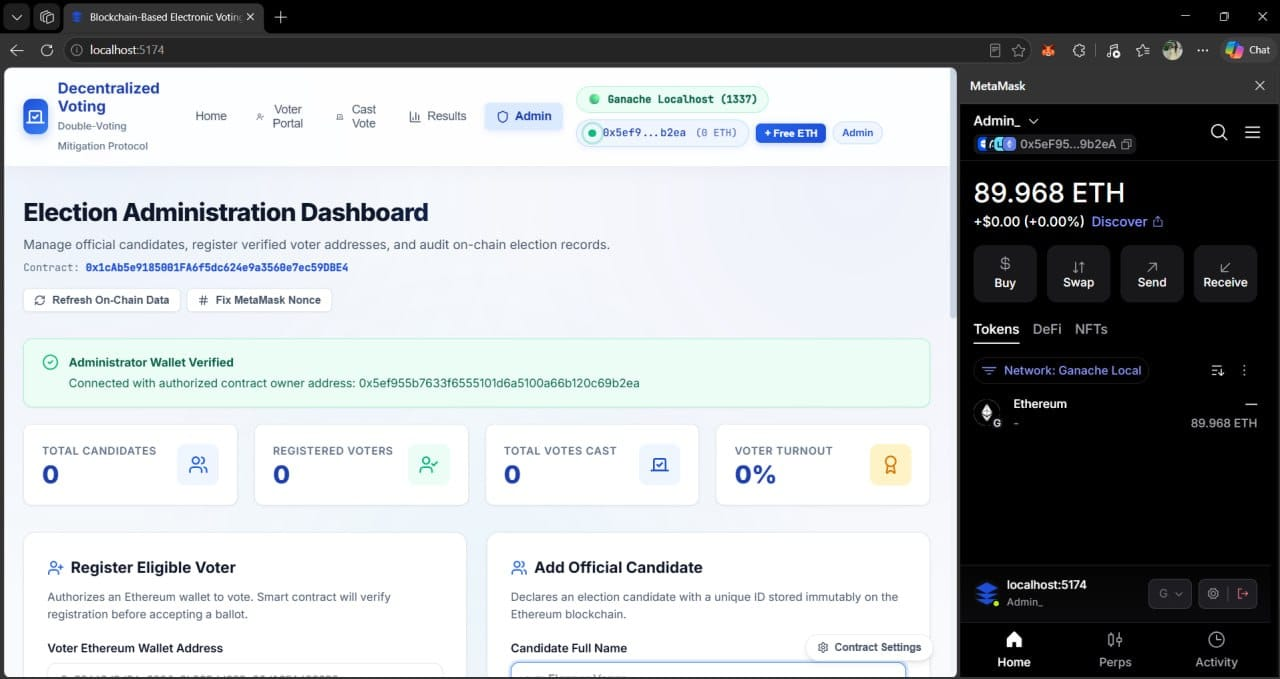
\includegraphics[width=\linewidth,height=3.4cm,keepaspectratio]{results/admin_dashboard.jpeg}
\captionof{figure}{Snapshot 2: Administrator dashboard.}
\end{minipage}
\end{figure}

\begin{figure}[H]
\centering
\begin{minipage}[t]{0.47\textwidth}\centering
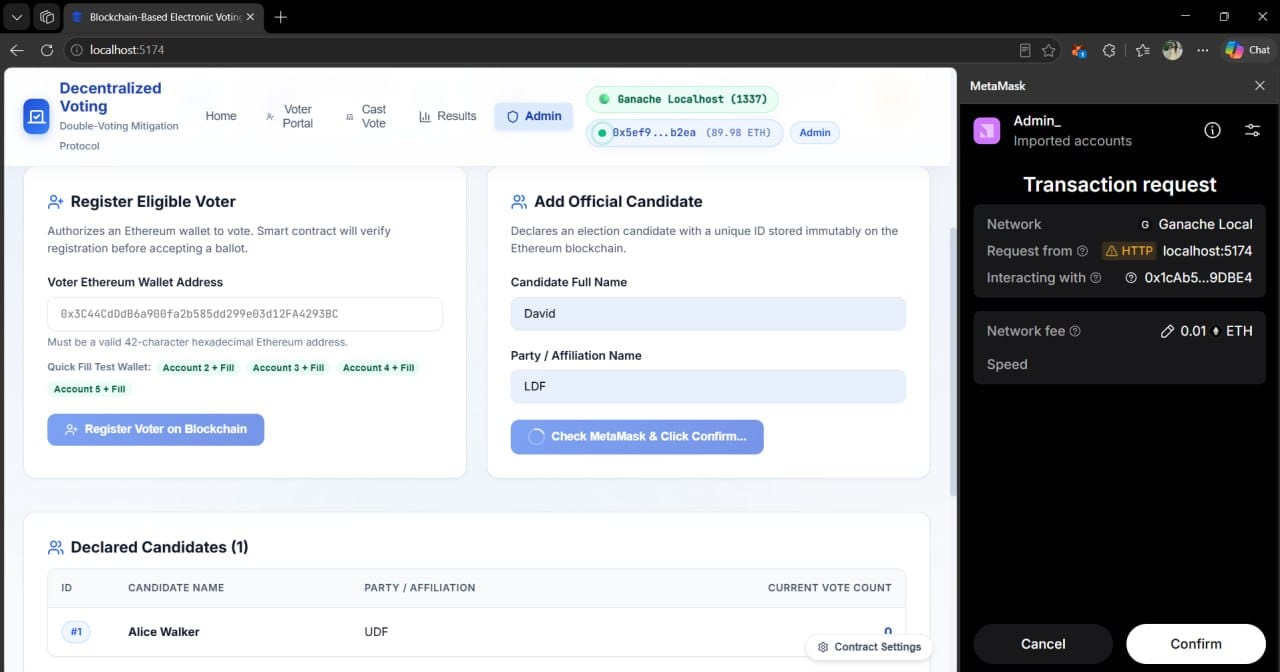
\includegraphics[width=\linewidth,height=3.4cm,keepaspectratio]{results/adding_candidate.jpeg}
\captionof{figure}{Snapshot 3: Candidate registration.}
\end{minipage}\hfill
\begin{minipage}[t]{0.47\textwidth}\centering
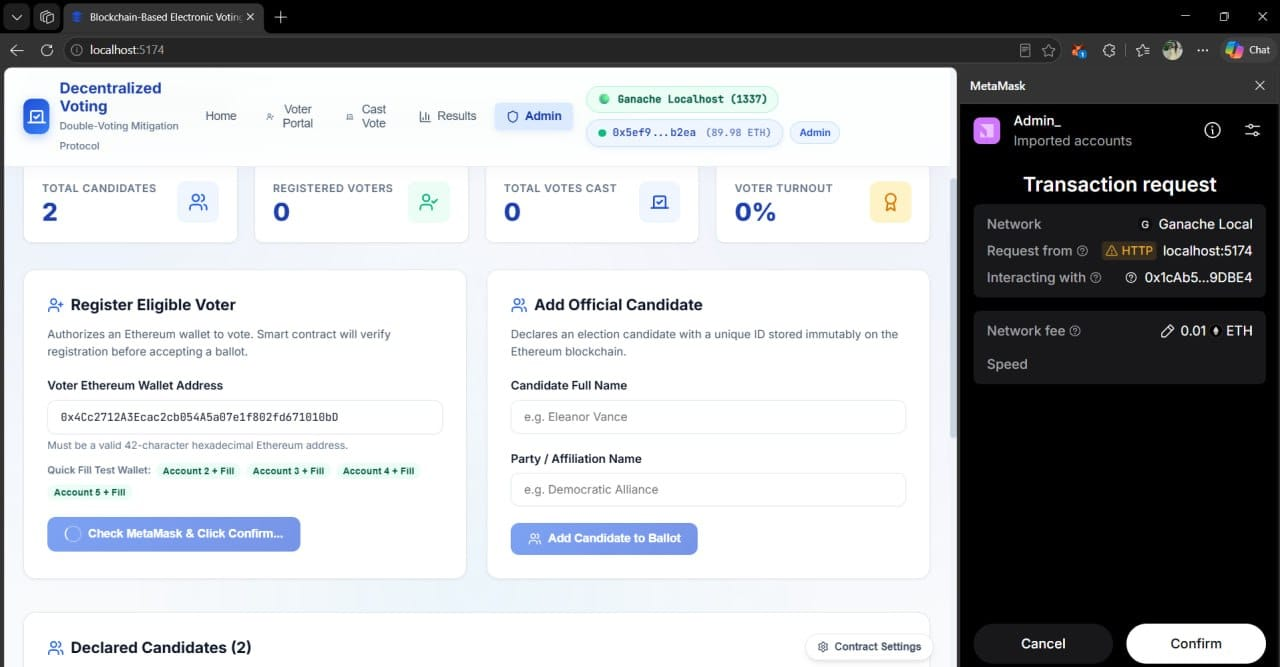
\includegraphics[width=\linewidth,height=3.4cm,keepaspectratio]{results/adding_voter.jpeg}
\captionof{figure}{Snapshot 4: Voter registration.}
\end{minipage}
\end{figure}

\begin{figure}[H]
\centering
\begin{minipage}[t]{0.47\textwidth}\centering
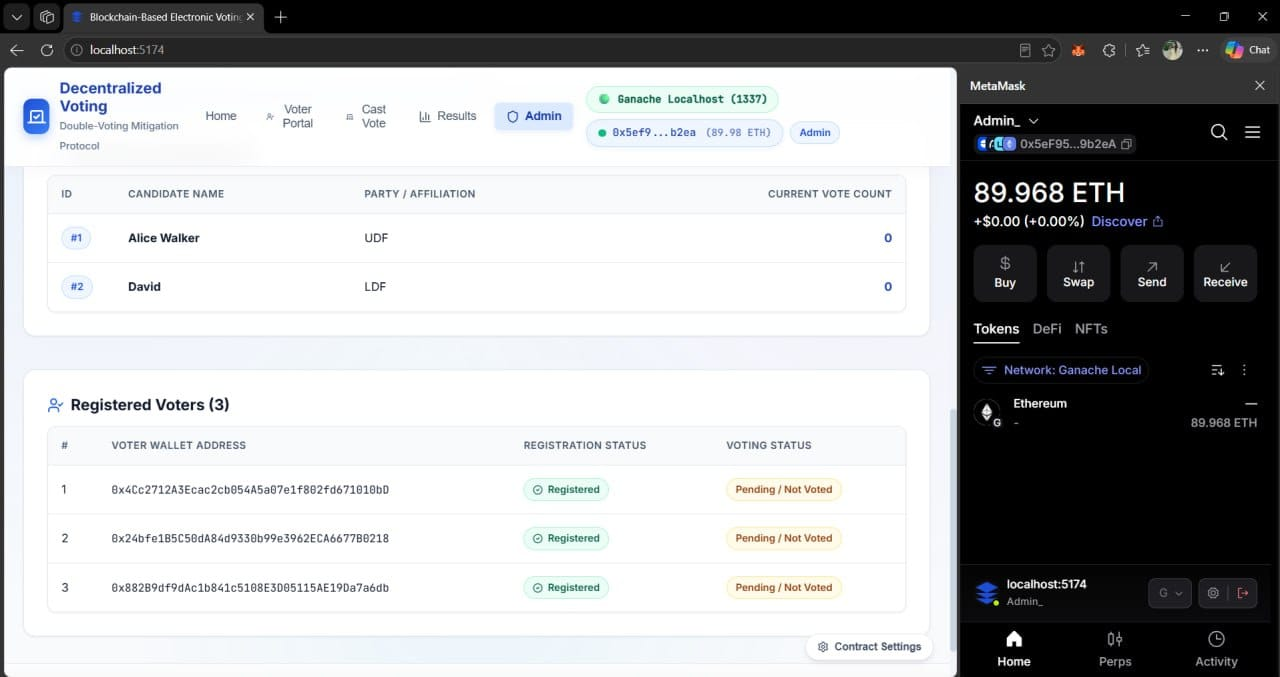
\includegraphics[width=\linewidth,height=3.4cm,keepaspectratio]{results/added_details.jpeg}
\captionof{figure}{Snapshot 5: Registered entities.}
\end{minipage}\hfill
\begin{minipage}[t]{0.47\textwidth}\centering
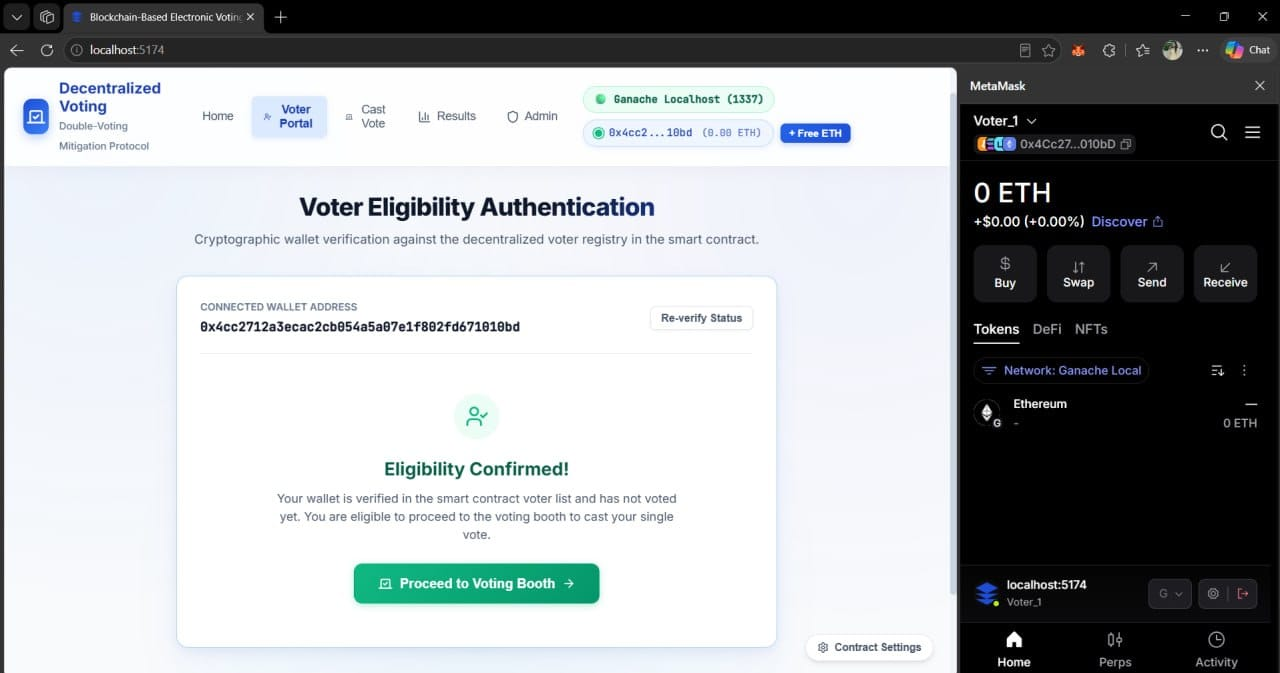
\includegraphics[width=\linewidth,height=3.4cm,keepaspectratio]{results/voter_verification.jpeg}
\captionof{figure}{Snapshot 6: Voter verification.}
\end{minipage}
\end{figure}

\begin{figure}[H]
\centering
\begin{minipage}[t]{0.47\textwidth}\centering
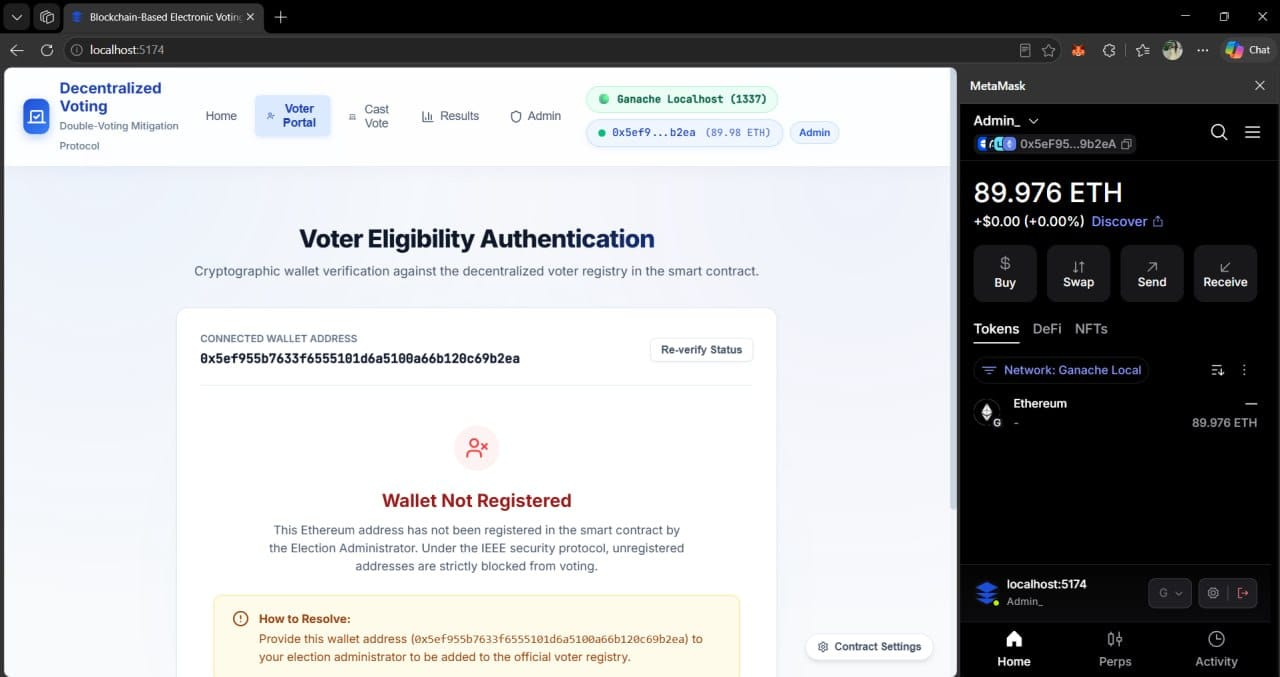
\includegraphics[width=\linewidth,height=3.4cm,keepaspectratio]{results/voter_page.jpeg}
\captionof{figure}{Snapshot 7: Unregistered voter rejection.}
\end{minipage}\hfill
\begin{minipage}[t]{0.47\textwidth}\centering
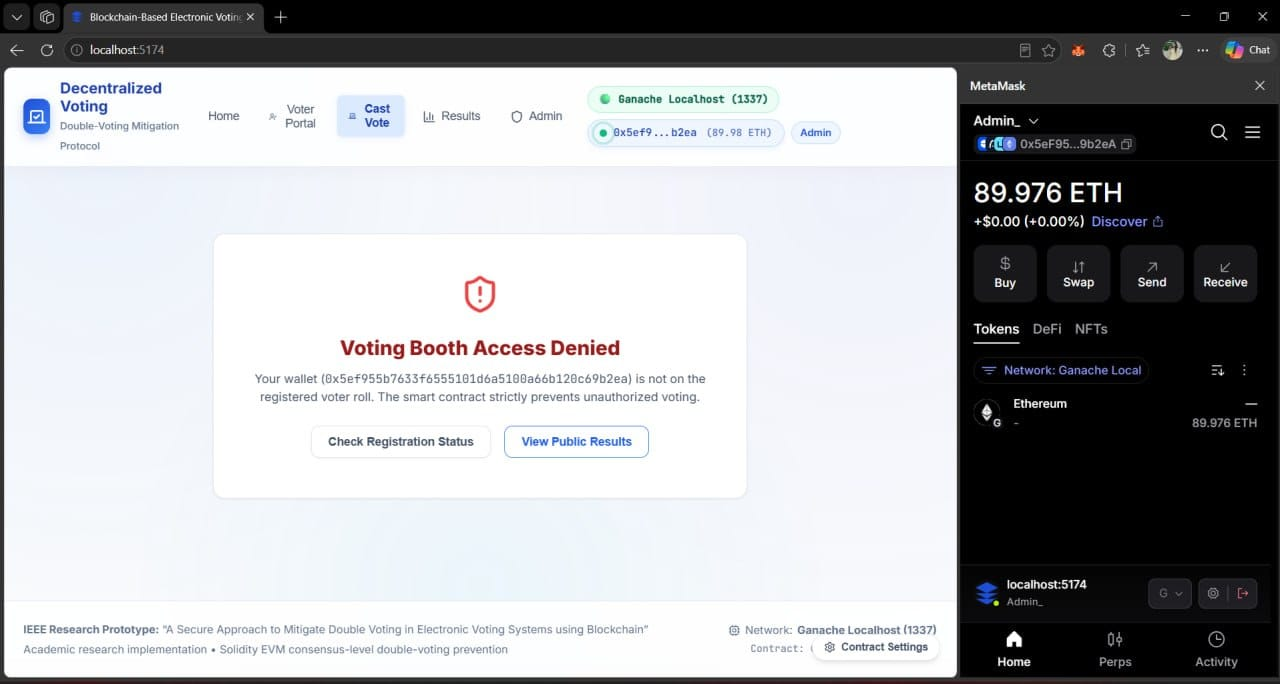
\includegraphics[width=\linewidth,height=3.4cm,keepaspectratio]{results/vote_casting_session.jpeg}
\captionof{figure}{Snapshot 8: Route access control.}
\end{minipage}
\end{figure}

\begin{figure}[H]
\centering
\begin{minipage}[t]{0.47\textwidth}\centering
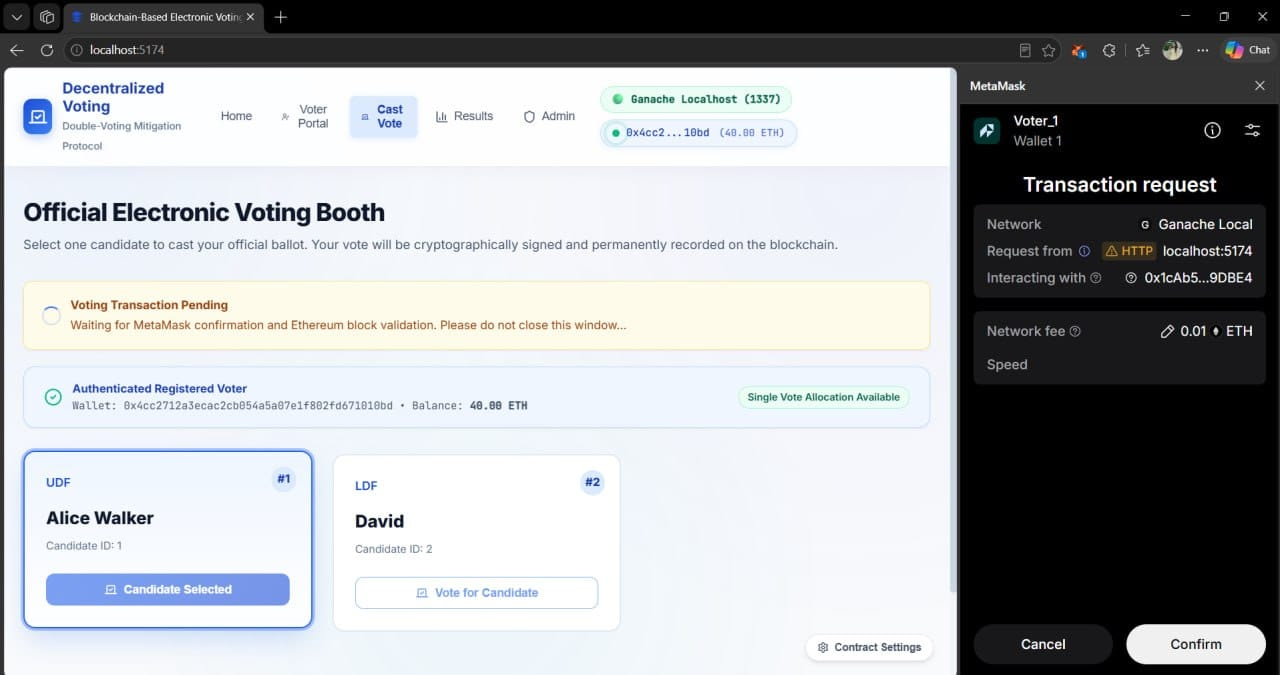
\includegraphics[width=\linewidth,height=3.4cm,keepaspectratio]{results/voting_booth.jpeg}
\captionof{figure}{Snapshot 9: Voting booth.}
\end{minipage}\hfill
\begin{minipage}[t]{0.47\textwidth}\centering
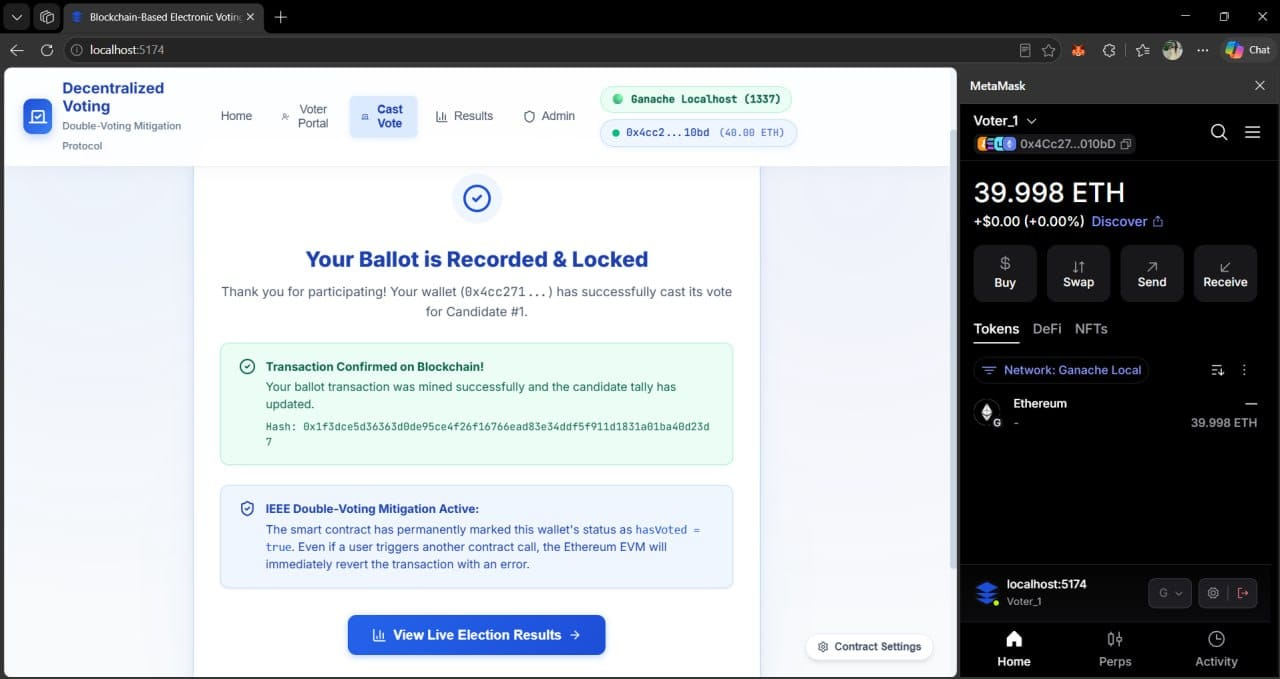
\includegraphics[width=\linewidth,height=3.4cm,keepaspectratio]{results/casted_vote.jpeg}
\captionof{figure}{Snapshot 10: Ballot confirmation.}
\end{minipage}
\end{figure}

\begin{figure}[H]
\centering
\begin{minipage}[t]{0.47\textwidth}\centering
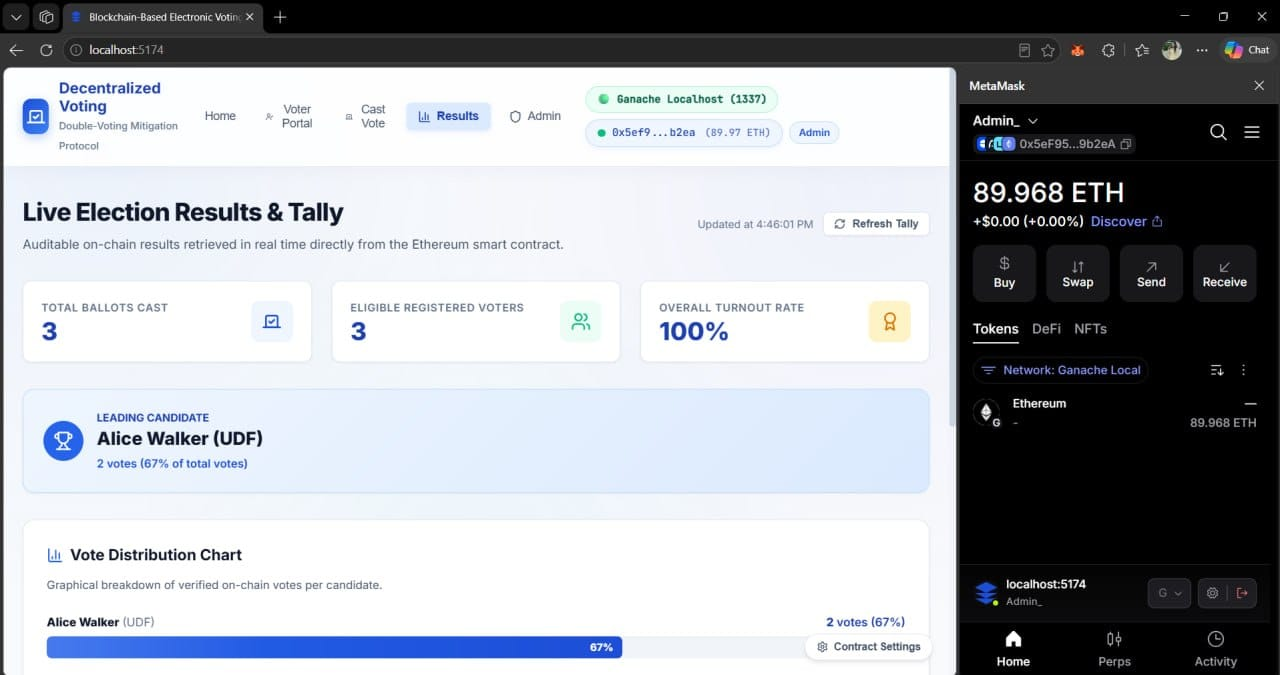
\includegraphics[width=\linewidth,height=3.4cm,keepaspectratio]{results/result.jpeg}
\captionof{figure}{Snapshot 11: Live election results.}
\end{minipage}\hfill
\begin{minipage}[t]{0.47\textwidth}\centering
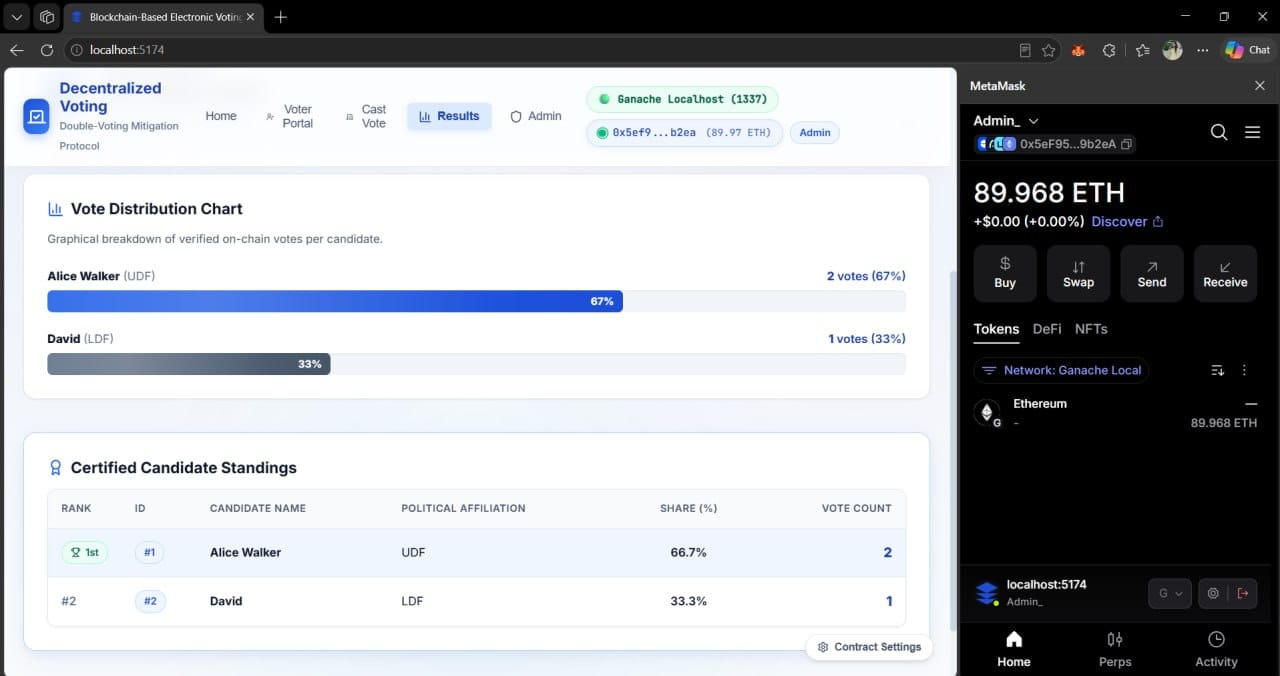
\includegraphics[width=\linewidth,height=3.4cm,keepaspectratio]{results/result_page2.jpeg}
\captionof{figure}{Snapshot 12: Certified standings.}
\end{minipage}
\end{figure}

\endgroup

%==============================================================================
% REFERENCES
%==============================================================================
\begin{thebibliography}{15}
\setlength{\itemsep}{2pt}
\setlength{\parskip}{0pt}

\bibitem{Asha2025}
P.~Asha, P.~G. Reddy, R.~A. Canessane, J.~Refonaa, L.~Padma Suresh, and R.~S. Nancy Noella, ``A Secure Approach to Mitigate Double Voting in Electronic Voting Systems using Blockchain Technology,'' in \emph{Proc. 2025 8th International Conference on Circuit, Power and Computing Technologies (ICCPCT)}, Kollam, India, 2025, pp. 115--120, doi: 10.1109/ICCPCT65132.2025.11176586.

\bibitem{Farooq2022}
M.~S. Farooq, U.~Iftikhar, and A.~Khelifi, ``A Framework to Make Voting System Transparent Using Blockchain Technology,'' \emph{IEEE Access}, vol.~10, pp. 54102--54118, 2022, doi: 10.1109/ACCESS.2022.3175783.

\bibitem{Shahzad2019}
B.~Shahzad and J.~Crowcroft, ``Trustworthy Electronic Voting Using Adjusted Blockchain Technology,'' \emph{IEEE Access}, vol.~7, pp. 24477--24488, 2019, doi: 10.1109/ACCESS.2019.2895670.

\bibitem{Kshetri2018}
N.~Kshetri and J.~Voas, ``Blockchain-Enabled E-Voting,'' \emph{IEEE Software}, vol.~35, no.~4, pp. 95--99, Jul./Aug. 2018, doi: 10.1109/MS.2018.2801546.

\bibitem{Seftyanto2019}
D.~Seftyanto, A.~Amiruddin, and A.~R. Hakim, ``Design of Blockchain-Based Electronic Election System Using Hyperledger: Case of Indonesia,'' in \emph{Proc. 2019 11th International Conference on Information Technology and Electrical Engineering (ICITEE)}, Pattaya, Thailand, 2019, pp. 1--6, doi: 10.1109/ICITEE.2019.8929965.

\bibitem{Ajao2025}
L.~A. Ajao, B.~U. Umar, H.~O. Ohize, E.~M. Dogo, E.~Esenogho, and M.~Cameron, ``Blockchain Integration With Multimodal Biometric Authentication System for Secure Smart Verifiable Electronic Voting System,'' \emph{IEEE Access}, vol.~13, pp. 14201--14220, 2025, doi: 10.1109/ACCESS.2025.3530012.

\bibitem{Mahmood2024}
W.~A. Mahmood, J.~Waleed, A.~R. Abbas, H.~Alaskar, M.~Altulyan, and A.~J. Hussain, ``Intelligent Gesture-Enhanced Blockchain Voting: A New Era of Secure and Accessible E-Voting,'' \emph{IEEE Access}, vol.~12, pp. 88310--88325, 2024, doi: 10.1109/ACCESS.2024.3418892.

\bibitem{PerezGarcia2021}
J.~C. P{\'e}rez Garc{\'\i}a, A.~Benslimane, and S.~Boutalbi, ``Blockchain-Based System for E-Voting Using Blind Signature Protocol,'' in \emph{Proc. IEEE Global Communications Conference (GLOBECOM)}, Madrid, Spain, 2021, pp. 1--6, doi: 10.1109/GLOBECOM46510.2021.9685957.

\bibitem{Baniata2025}
H.~Baniata and G.~Caluna, ``BP-Vot: Blockchain-Based e-Voting Using Smart Contracts, Differential Privacy, and Self-Sovereign Identities,'' \emph{IEEE Transactions on Emerging Topics in Computing}, vol.~13, no.~1, pp. 45--58, Jan.--Mar. 2025, doi: 10.1109/TETC.2024.3411200.

\bibitem{Benabdallah2022}
A.~Benabdallah, A.~Audras, L.~Coudert, N.~El Madhoun, and M.~Badra, ``Analysis of Blockchain Solutions for E-Voting: A Systematic Literature Review,'' \emph{IEEE Access}, vol.~10, pp. 70746--70759, 2022, doi: 10.1109/ACCESS.2022.3187688.

\bibitem{Quzmar2021}
A.~Quzmar, M.~Qatawneh, and S.~Al-Maaitah, ``E-Voting System Based on Blockchain Technology: A Survey,'' \emph{International Journal of Computer Applications}, vol.~183, no.~42, pp. 1--10, Nov. 2021.

\bibitem{Sah2025}
A.~Sah, A.~Kumar, and B.~Bhushan, ``Leveraging Blockchain Technology for Secure Online Voting Systems: A Comprehensive Review,'' \emph{Journal of Network and Computer Applications}, vol.~222, p. 103810, Feb. 2025, doi: 10.1016/j.jnca.2024.103810.

\bibitem{Barelli2025}
R.~Barelli, M.~D'Onghia, and S.~Longari, ``Toward Secure Electronic Voting: A Survey on E-Voting Systems and Attacks,'' \emph{ACM Computing Surveys}, vol.~57, no.~2, pp. 1--38, Feb. 2025, doi: 10.1145/3698780.

\bibitem{Wermelinger2026}
C.~C. Wermelinger, A.~M. Mariano, and J.~M. da Silva, ``Trust and Security in Critical Digital Infrastructures: A Conditional Analysis of Acceptance and Intention to Change in Electronic Voting Systems,'' \emph{Government Information Quarterly}, vol.~43, no.~1, p. 101890, Jan. 2026, doi: 10.1016/j.giq.2025.101890.

\bibitem{Chaudhary2023}
S.~Chaudhary, S.~Shah, R.~Kakkar, R.~Gupta, A.~Alabdulatif, S.~Tanwar, G.~Sharma, and P.~N. Bokoro, ``Blockchain-Based Secure Voting Mechanism Underlying 5G Network: A Smart Contract Approach,'' \emph{IEEE Access}, vol.~11, pp. 60521--60535, 2023, doi: 10.1109/ACCESS.2023.3285149.

\end{thebibliography}

\end{document}
